%%% Local Variables:
%%% mode: latex
%%% TeX-master: t
%%% End:

\documentclass[doctor,openright]{tongjithesis}
% \documentclass[%
%   master|doctor, % mandatory option
%   xetex|pdftex|dvips|dvipdfm, % optional
%   secret,
%   openany|openright,
%   arialtoc,arialtitle]{tongjithesis}

% % 所有其它可能用到的包都统一放到这里了,可以根据自己的实际添加或者删除。
\usepackage{tongjiutils}
\usepackage[top=2.54cm, bottom=2.54cm, left=3.17cm, right=3.17cm]{geometry}
%\newcommand{\citeA}[1]{\citeauthor{#1}, \citeyear{#1} \cite{#1}}
%\newcommand{\citeB}[1]{(\citeauthor{#1}, \citeyear{#1} \cite{#1})}

% 你可以在这里修改配置文件中的定义,导言区可以使用中文。
\def\myname{邱君诚}

\begin{document}

% 定义所有的eps文件在 figures 子目录下
\graphicspath{{figures/}}


\frontmatter

%%% Local Variables:
%%% mode: latex
%%% TeX-master: t
%%% End:
\secretlevel{保密} 
\secretyear{2}

\ctitle{基于弹性波模式解耦的全波形反演方法}

% 按照申请工学学位设计。如有其它需要,请修改相应文字。
\makeatletter
  \iftongji@doctor
    \cdegree{博士}
  \else
    \iftongji@master
      \cdegree{理学硕士}
    \fi
  \fi

\makeatother

\cdepartment{同济大学海洋学院}

\cmajorfirst{固体地球物理}

\degtype{理学}

\cauthor{王腾飞}

\cstnr{1110701}

\csupervisor{程玖兵 教授}

% 如果没有副指导老师或者联合指导老师,把各自{}中内容留空即可。

\cassosupervisor{}

\ccosupervisor{}

% 日期自动生成,如果你要自己写就改这个cdate
%\cdate{\CJKdigits{\the\year}年\CJKnumber{\the\month}月}
\makeatletter
  \iftongji@doctor
    \edegree{Doctor of Philosophy}
  \else
    \iftongji@master
      \edegree{Master of Science}
    \fi
  \fi

\makeatother

%\cfunds{自然基金项目(No.123456789)}

%\efunds{(Supported by the Natural Science Foundation of China for\\ Distinguished
%         Young Scholars, Grant No.123456789)}

\etitle{Elastic full waveform inversion based on wave mode decomposition}

\edepartment{School of Ocean and Earth Science}

\edispline{Natural Science}

\emajorfirst{Solid Geophysics}
%\emajorsecond{TONGJILUG}

\eauthor{Tengfei Wang}

\esupervisor{Prof. Jiubing Cheng}

% 这个日期也会自动生成,你要改么?
% \edate{May, 2009}

% 定义中英文摘要和关键字
\begin{cabstract}
	通过地震数据定量地估计介质参数甚至岩石物理参数是探测地球内部结构和勘探油气资源的主要任务。随着计算能力的快速提升以及
	长偏移距、宽方位、宽频带的地震数据采集技术的成熟,旨在估计全波数谱速度模型的全波形反演(FWI)方法
	成为地震勘探中强有力的工具。然而在实际中,FWI无法获得理论上预期的问题解决能力。近几十年来,
	为了解决FWI受到初始模型不够好、数据中缺乏低频导致的周波跳跃(cycle-skipping),克服子波估计不准以及噪音影响等问题的困扰,
	许多学者发展了分频率、分偏移
	距、分散射角等多尺度策略来降低非线性程度。此外,在弹性介质中,
	不同波模式转换及其他多分量数据的复杂性
	进一步增加了反问题的非线性程度,而且
	不同参数扰动的偏导数波场在特定散射角范围内的重叠还会导致参数耦合效应。
	为了重建不同波数谱的模型,本文围绕模式解耦这一数据分离工具,从弹性波全波形反演(EFWI)、弹性波波动方程反射走时反演
	(EWERTI)以及弹性波最小二乘逆时偏移(ELSRTM)出发,尝试恢复高波数、中低波数以及全波数成分的弹性模型参数,进而形成弹性波
	反演中较完整的工作流程体系。

%	在第二章中主要讨论EFWI中模式解耦对压制参数耦合效应的作用。
	EFWI通过最小化观测到的多分量数据与正演模拟数据
	之间的残差来获得高分辨率的地下弹性参数模型。由于Hessian矩阵的显式计算与求逆代价十分
	巨大,实际应用中的大规模问题通常采用梯度类的最优化方法而非基于Hessian的方法。然而,多参数
	反演中的参数耦合效应会引起不同参数间梯度的串扰,进而会严重影响反演的收敛速度与精度。
%	近期,弹性波模式解耦的方法被用来对梯度进行预条件从而降低EFWI过程中的参数耦合
%	问题。
	第二章提出了一种基于模式解耦的EFWI方法,该方法在时间域通过正传
	与解耦的反传波场之间的互相关来获得梯度。文中基于解耦的Frech$\acute{e}t$导数来分析
	Hessian矩阵和分辨率矩阵的性态,并对比常规共轭梯度法、Gauss-Newton法和模式解耦法三者梯度之间的异同来解释模式解耦压制参数耦合的物理机制。
	简单流体饱和模
	型与Marmousi-II模型的数值实例,证明了模式解耦的预条件共轭梯度法(MDPCG)可以降低P-波和S-波速度($V_p$和$V_s$)
	之间的参数耦合,在不涉及Hessian计算的情况下获得快速收敛。

	利用弹性反射波波形反演(ERWI)可以更新中深层模型的中低波数成分,从而为EFWI提供较好的初始模型。
	然而,波形匹配的ERWI也同样会面临周波跳跃的问题。相比波形匹配的目标函数,反射走时目标函数与背景速度模型之间具有
	更加线性的关系。因此第三章中采用弹性波波动方程反射走时反演(EWERTI),
	通过DIW(Dynamic image warping)算法来提取走时残差并以此建立目标函数,
	可以一定程度上回避周波跳跃。
	文中采用基于模式解耦的两步反演策略,首先采用PP波数据反演$V_p$,然后固定反演好的$V_p$通过PS波反演$V_s$。
	地面P/S数据分离可获得不同模式数据残差,空间域弹性波模式解耦则可以对梯度有效地预条件,从而实现$V_p$和$V_s$的分步反演,这将有效降低反演的非线性程度。
	反射波波路径核函数分析解释了解耦的波模式反射路径对压制串扰的重要作用。
%	局部倾角导引正则化约束可以使得反演快速收敛到具有地质意义的模型。
	此外,
	为了降低反演的多解性、保证反演够获得更合理的速度模型,采用包含地层倾角信息的成像结果进行局部倾角导
	引正则化来确保反演获得更符合地质意义的速度模型。
	文中采用Sigsbee2A模型来
	验证EWERTI方法以及反演策略的有效性,并用EFWI检验EWERTI反演结果的准确性。

	ELSRTM旨在通过拟合反射波振幅信息来反演弹性参数模型的高波数成分,可视为线性的EFWI问题。
	常规ELSRTM通过多次迭代可以压制由于数据缺失、粗网格采样等产生的成像噪音,提高成像分辨率,同时部分地降低参数间的耦合
	效应。模式解耦则可以在计算梯度时通过分离出S波梯度,使得ELSRTM中S波速度扰动的反演接近于单参数反演,降低反演参数耦合及非线性程度
	。由此,针对不同的参数耦合情况设计了相应
	的反演策略来压制参数耦合。在$V_p$较少受$V_s$耦合影响时,采用梯度解耦双参数同时反演;而在$V_p$与$V_s$强烈相互影响时,先采用解耦通过S波
	反演好$V_s$,然后反演$V_p$,这样可以进一步压制$V_p$所受到的来自$V_s$的耦合影响。
%	另外,由于实际反射数据与Born模拟数据之间存在差异,因此在ELSRTM中最好能匹配反射数据与背景波场之间的残差。

%	为了恢复弹性介质模型中的不同波数成分,本文
	本文针对弹性波反演问题,分别从EFWI,EWERTI以及ELSRTM
	三个方面入手来恢复不同波数成分的弹性参数模型。在常规多尺度策略的基础上,通过空间域模式解耦和地面P/S分离
	获取P或S数据子集来适应反演中的不同需求。根据解耦的P/S波数据在Frech$\acute{e}t$导数、
	Hessian和分辨率矩阵以及Born反射波路径计算中的贡献和影响,设计出适用于不同阶段的梯度预条件方式和多尺度策略,
	从而降低弹性波反演的非线性和参数耦合程度,
	并形成完整的弹性波反演体系,获得从浅部到深部更准确的弹性参数估计。


\end{cabstract}

\ckeywords{全波形反演,Hessian和分辨率矩阵,参数耦合,波动方程反射走时反演,反射波路径核函数,最小平方逆时偏移,弹性波,模式解耦}

\begin{eabstract}
	The primary task of the detection and exploration of the Earth's interior is to estimate the elastic parameters or rock properties
	quantitively
	through the recording data on the surface. With the developement of 
	high-performance computation ability and the
	maturation of wide-azimuth, long-offset and broadband data accquisition 
	technology, full waveform inversion (FWI) becomes a powerful tool to recover the full
	 wavenumber spectrum of the subsurface. However, FWI can not provide the estimated
	model as good as expected. In order to overcome the obstacles such as bad initial models,
	insufficiency of low frequency component in the data, inaccurately estimated source
	wavelet, low sigal/noisy ratio in the data, many researchers developed hierarachical strategies
	by selecting data subsets of different frequency, offset or scattering-angle during the
	inversion.	
	In elastic media, complicated mode conversions and other multicomponent problems further increase the
	nonlinearity of inversion. Besides, in certain angles, the overlapped partial derivative wavefields of  different
	parameter will lead to trade-offs.
	To rebuild the model containing different wavenumber spectrum, elastic full waveform
	inversion (EFWI), elastic wave equation 
	reflected traveltime inversion (EWERTI) and elastic least square reverse time
	migration (ELSRTM) are implemented with the help of wave mode decomposition, in which we
	try to recover the low and intermediat wavenumber, 
	the high wavenumber and the full wavenumber spectrum of the elastic model.

Elastic full waveform inversion (EFWI) aims to reduce the misfit between recorded and modelled multi-component
seismic data for deducing a detailed model of elastic parameters in the subsurface.
Because the explicit computation and inversion of the Hessian matrix
is extremely resource intensive,
a gradient-based (rather than Hessian-based) minimization is generally applied for large-scale applications.
However, the multi-parameter trade-off effects cause cross-talks in the computed gradients and
thus severely affect the convergence and the quality of the inverted model.
%Recently, preconditioning the gradients based on elastic wave mode decomposition
%has been suggested for mitigating the parameter trade-offs in the EFWI process.
In the second chapter, we propose a mode decomposition (MD)-based EFWI approach, in which the preconditioned gradients
are obtained through the cross-correlation of the forward and
decomposed adjoint wavefields in the time domain.
Based on the decomposed Frech{$\acute{e}$}t derivatives,
we explain the mechanism of this approach through analyses of Hessian and resolution matrices
and comparisons with the Gauss-Newton gradients.
Numerical examples of a simple fluid-saturated model and the Marmousi-II model
demonstrate that the MD-based preconditioned conjugate-gradient approach
can mitigate the trade-off between the P- and S-wave velocities and achieve fast
convergence without any Hessian-involved calculations.

Elastic reflection waveform inversion (ERWI) utilize the reflections to update the low and
intermediate wavenumber in the
deeper part of model, which can provide good initial models for EFWI. However, ERWI suffers from
the cycle-skipping problem due to the objective function of waveform fitting. Since taveltime
information relates to the background model more linearly, the cycle-skipping of traveltime
objective function will be less severe
compared with the previous one. Thus, in the third chapter we implement the WERTI by using the $L_2$ norm of the traveltime
residual extracted by the Dynamic image warping (DIW) as objective function.
The reflection kernel analysis shows that mode decomposition can suppress the artifacts in
gradient calculation. 
Besides, the model regularization through local dip-dependent smooth filter ensures the inversion converging to a
geological model. 
Based on that, a two-step inversion strategy is adopted, in which PP reflections are first used to invert $V_p$,
followed by $V_s$ inversion with PS reflections based on the well recoverd $V_p$. P/S
separation of multicomponent seismograms provides P or S recordings while spatial wave mode
decomposition provides P or S wavefields, which help
to  reduce the nonlinearty of inversion effectively.
%The kernel of reflection wavepath proves that mode decomposition can surpress the artifacts in
%the reflection inversion. 
Numerical example of Sigsbee2A model validates the effectiveness of the
algorithms and strategies for elastic WERTI (E-WERTI).
%Numerical example of Sigsbee2A model validates the effectivenss of the 
%algorithms and strategies for EWERTI, whose results also are tested through EFWI.

ELSRTM is a linearized EFWI aimming to fit the waveform of reflections generated by the inverted
high-wavenumber perturbations. 
%Due to the energy difference between Born and reflection data, it is
%more suitable to match the residual between reflection data and the background data during ELSRTM.
LSRTM can suppress the imaging artifacts caused by reduce migration artifacts arising
from limited aperture, coarse sampling, and acquisition gaps. Conventional ELSRTM can sligthly but
not entirely mitigate the parameter trade-offs. 
Nonetheless, mode decomposition
isolates the S-wave part gradient, which makes the inversion of S-wave velocity
perturbation a mono-parameter inversion to help mitigate the trade-offs. In the fourth chapter, we
design different inversion strategies to cope with the different situations. When $V_p$ is little
affected by $V_s$, we invert the two parameter simultaneously with mode decomposition; when $V_p$
and $V_s$ couple with each
other severely, we recommand inverting $V_s$ firstly followed by $V_p$ inversion to further mitigate
the trade-offs from $V_s$ during the $V_p$ inversion.

In this thesis, we focus on the mode-decomposition-based inversion methods to recover the model
containing different wavenumber spectrum. P/S separation of multicomponent data and wave mode
decomposition provide flexible P or S wave data in different stage of inversion.
Investigation of decomposed Frechet derivative, Hessian and resolution matrices and Born reflection
kernel show the different contribution of P or S wave to gradients. Accordingly, hierarchical
strategies are designed to reduce the nonlinearty, trade-off
effects and other problems during inversion and finally rebuild the elastic model from shallow to
deep more effectively. 

\end{eabstract}

%\ckeywords{全波形反演,Hessian和分辨率矩阵,参数耦合,波动方程反射走时反演,反射波路径核函数,最小平方逆时偏移,弹性波,模式解耦}
\ekeywords{Full waveform inversion, Hessian and resolution matrix, parameter trade-off, 
	wave equation reflected traveltime inversion, kernel of reflection wavepath, least-square RTM,
	Elasticity, Mode decomposition}

\makecover


% 目录

\tableofcontents

\begin{denotation}
\item[GNU] GNU's Not Unix /'gnu:/
\item[GFDL] GNU Free Documentation License
\item[GPL] GNU General Public License
\item[FSF] Free Software Foundation
\item[SMP] 对称多处理
\item[API] 应用程序编程接口
\item[$E$] 能量
\item[$m$] 质量
\item[$c$] 光速
\item[$P$] 概率
\item[$T$] 时间
\item[$v$] 速度
\end{denotation}


%\listoffigures

%\listoftables

%\listofequations

%%% 正文
\mainmatter
%\chapter{引言}
\section{研究背景和意义}
地震勘探的主要目标是通过观测的地震数据来推断地下结构以及定量地估计介质参数。
弹性参数,包括纵波(P波)速度、横波(S波)速度以及密度等参数,可以通过岩石物理这一桥梁转换为岩石物性参数,从而获得储层及其围岩的岩石性质。这对油气田的勘探、
开发以及二氧化碳(CO$_2$)填埋动态监测等具有重要意义。传统地震数据处理中,通常用声波方程来描述地震波在地下介质中的传播。而地下介质的真实情况往往要复杂得多,
需要通过考虑弹性
、各向异性甚至衰减的波动方程来更准确地描述波的传播。但是介质模型越复杂,所引入的计算量就越大,
所对应的多参数反问题也越困难。目前来看,从声介质过渡到弹性介质能够以较小的代价来获取较准确的模型表征。
尽管从声波近似过渡到弹性近似会成倍地增加计算量,但是这对多分量地震数据的成像或反演显然十分必要。考虑弹性效应的数据处理流程能区分并利用数据中的
P波与S波模式,因此可以充分利用弹性全波场信息改善气云区成像、岩性估计、流体识别以及裂缝与应力场的刻画等。
近年来,岩性油气藏(如致密砂岩、页岩)勘探技术极大地依赖于弹性参数估计,这使得考虑地震波的弹性乃至各向异性效应都具有重要意义。

地震勘探中的诸多过程都非常依赖于速度模型的精度,例如叠前深度偏移、振幅随偏移距变化(AVO)分析等都需要准确的背景速度模型。
因此,如何准确地获取高分辨率的速度模型是地震勘探中最为迫切的任务。
为了降低地震数据与模型参数之间的非线性程度,Claerbout (1985)\cite{Claerbout1985Imaging}将速度模型分解为两个部分:1)描述速度(阻抗)界面的高频部分;
2)控制波传播走时的中低频部分。这样的分解对应于地震勘探中最核心的两个任务,即偏移成像与速度建模。传统方法中,偏移成像和AVO
反演通常用来获取模型的高频部分,
而偏移速度分析(MVA)和走时层析被用来恢复模型的低频部分。但是地面地震反射数据的有限观测孔径以及子波的带限效应使得
这类方法所能恢复的波数谱上存在明显的缺口。如图\ref{fig:GapInSeisVel},
MVA与走时层析只能恢复波数非常低的成分,而偏移成像只能获得有限带宽的高波数信息。
为此,人们也在研究各种方法来尽可能填补速度反演中的波数谱缺口。基于射线理论,有学者尝试采用高分辨率走时层析来拓宽低波数部分的反演能力,
采用真振幅和最小平方偏移方法拓展对高波数成分的反演能力。
但是以上基于射线理论的方法,在模型复杂区域很难处理多路径及焦散等问题。
近年来,随着高性能计算能力的不断提升,基于波动理论的速度反演方法由于可以避免上述问题并具有更高的分辨能力而受到越来越多的关注。
目前基于波动理论的反演方法主要有以下三类:
%许多学者尝试采用高分辨率走时层析、波动方程速度分析(WEMVA)等方法扩展低波数部分的频带,而高波数部分则采用真振幅和最小平方偏移方法来获取更高精度和更宽波数范围的结果。
%同时,更具潜力的全波形反演方法(FWI)采用全波场信息能够获得具有更连续波数谱的地下模型。
\begin{figure}[t] 
   \centering 
   \subfloat{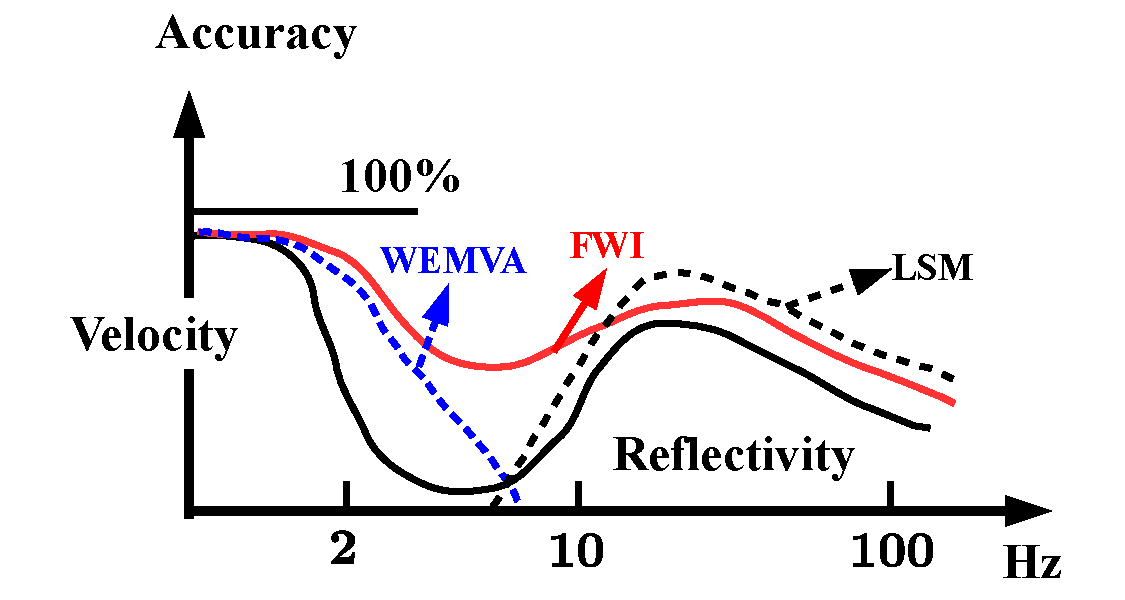
\includegraphics[width=1.00\textwidth]{Figure/chapter01/WavenumberGap2.pdf}}
   \caption{地震数据所能恢复的频带示意图。传统走时层析+偏移成像的方式所恢复的速度模型有明显的中低频缺口,
	   WEMVA和LSM方法有助于拓展低波数与高波数部分的带宽,而FWI则尝试恢复更连续的波数谱(引自Claerbout, 1985\cite{Claerbout1985Imaging})。}
   \label{fig:GapInSeisVel}
\end{figure}

%传统方法中大多基于射线理论进行成像与速度估计,这在模型复杂区域很难处理多路径以及焦散等问题,基于波动理论则可以避免上述问题。
%目前基于波动理论的反演方法主要有以下三类:

1、全波形反演(FWI):该方法通过匹配数据中携带的所有信息,包括走时、振幅、模式转换甚至多次波等,来获得对地下模型全波数谱的
恢复。
相比走时层析和MVA,它可以获取更高分辨率的地下模型。
自从Lailly (1983)\cite{lailly1983seismic}和Taratola
(1984)\cite{tarantola1984}建立了FWI理论框架之后,随着长偏移距、宽方位数据采集的推广,FWI
被认为是填补速度模型中尺度波数缺口最有潜力的工具。
但是FWI也受到众多因素的制约,如初始模型不够好或者数据缺少低频分量时产生的周波跳跃问题(cycle-skipping)、
地面观测数据导致的有限观测孔径问题、地下实际介质的粘弹性和各向异性问题以及高昂的计算代价等等。因此近二十年来,人们一方面尝试采用宽频震源、
鬼波压制等手段获得更加宽频的地震数据,另一方面尝试从目标函数选取、多尺度反演策略等方面降低上述问题的困扰。即便如此,FWI技术的推广应用扔存在许多挑战。

2、波动方程偏移速度分析(WEMVA):该类方法旨在更新背景速度模型,即模型的中低波数成分。
目前主流的做法通常利用地震数据中的反射波信息,通过构建反射波波路径并沿该路径来合理地更新模型中深部。
根据目标函数的残差类型,WEMVA可以分为数据域反演(如Xu et al., 2012\cite{xu:2012};Wu and Alkhalifah,
2015\cite[]{Wu2015b}; Zhou et al,
2015\cite[]{zhou:2015}; Chi et al, 2015\cite{chi2015})和
扩展成像域反演(如Sava and Fomel, 2006\cite{Sava2006}; Almomin and Biondi, 2012\cite{Almomin2012})。
前者采用观测数据与模拟数据间的走时、振幅等信息作为目标函数,后者则通过最大化扩展域成像道集零偏移距的能量来定义收敛准则。
它们与基于射线理论的成像域层析与数据域(非线性)层析方法有许多类似之处,但避免了传统层析流程中繁琐的人工拾取工作。不过,它们
还是会在一定程度上受到cycle-skipping等问题的困扰。

3、最小平方逆时偏移(LSRTM):该方法可以看作是线性化的FWI。在初始模型足够好的时候通过匹配模拟数据与观测数据的振幅来获得地下反
射系数模型。常规偏移成像
采用伴随算子来近似正传算子的逆,从而近似地获得反射率的成像结果。
但是伴随算子通常近似程度太大,所以有学者提出利用最小平方偏移(LSM)迭代获取越来越合理的正传算子的伪逆((Nemeth
et al., 1999\cite{Nemeth1999}; Kühl and Sacchi, 2003\cite{KuehlEtAl2003};
Dai et al.,
2012\cite{DaiEtAl2012})。
其本质上是通过最小化数据残差施加目标函数对模型二阶导数(Hessian)的信息
来获得二阶的收敛效果,从而获得更好的参数扰动反演结果。

重建地下介质的弹性参数模型对地球内部探测与油气藏的勘探至关重要。
相比声波FWI,
弹性波全波形反演(EFWI)能够自动考虑多分量数据中的各种弹性效应并反演得到地下介质的弹性参数,如P波速度($V_p$)和S波速度($V_s$)和密度($\rho$)。
然而在地震反演中考虑弹性效应会大大增加反问题的非线性程度,而且多参数反演
也会受到参数耦合(trade-off)效应的影响,因此
从声波近似过渡到弹性近似使得计算量和反演的困难程度成倍增加。
近年来,
由于计算机能力提升、多分量观测数据的增多,为了解决声波FWI无法回避的问题,考虑弹性甚至各向异
性的全波形反演逐渐成为研究热点。

多分量地震数据中同时含有P波和S波,这两种不同波模式对地下介质有着不同的刻画能力。
FWI中广泛采用的多尺度策略(分频率、分偏移距、分时窗和分散射角)本质上是选取不同的数据子集来逐步加入到反演中。
董良国等(2015)\cite{董良国2015}
指出在FWI过程中,不同的反演阶段采用不同的数据子集可以降低反演的非线性程度。而在弹性波反演中,更加需要根据不同参数
采用不同的数据子集或者不同的反演阶段
采用不同的数据子集,来降低多参数反演的非线性程度,同时也压制参数间的trade-off效应。
近年来不断发展的弹性波波模式分离技术能够提供准确的P或S波数据子集(Zhang and McMechan,
2010\cite{zhang.mcmechan:2010}; Cheng and Fomel,
2014\cite{cheng:2014b}; Li et al., 2016\cite{Li2016a}; Cheng et al.,
2016\cite{cheng:2016}),并已在弹性波逆时偏移(ERTM)中发挥重要作用(Wang et al.,
2016\cite{wang2016scalar})。
这些研究为弹性波反演中采取更多的多尺度策略带来新的机会(Wang et al., 2015\cite{wang:2015}; Ren and
Liu, 2016\cite{ren.liu:2016})。
在弹性框架下,EFWI目的在于构建高分辨率的弹性参数模型,EWERTI则利用弹性波走时信息构建背景速度模型,而ELSRTM是在可靠的背景模型基础上得到
高分辨率的地下反射界面图像。
本文借助模式解耦形成的波场分量或数据子集,实现新的更灵活的多尺度EFWI、EWERTI和ELSRTM方法,以期更准确地估计弹性参数模型的高、中、低波数成分,
为地球内部成像与油气资源勘探提供更好的支撑。

%通过模式解耦获取P或S波数据并根据
%需要加入到不同的反演阶段中,
%这种策略将贯穿始终,
%模式解耦将在EFWI,弹性波波动放程反射走时反演(EWERTI)以及ELSRTM中提供的分离的P或S波数据,来帮助获得更好的反演结果。
\section{研究现状}
\subsection{弹性波全波形反演研究现状}
Claerbout
(1971\cite{Claerbout1971})采用爆炸反射面的概念解释了地震偏移如何对地下构造进行刻画。Lailly
(1983)\cite{lailly1983seismic}
和Tarantola (1984)\cite{tarantola1984}最早用观测数据与模拟数据间波形残差的$L_2$范数作为目标函数,将偏移成像转化为
最优化问题,即FWI问题。该反问题的梯度(方向)可以采用伴随状态法通过入射波场与伴随波场之间的互相关来快速获得。FWI试图将宏观速度模型的
建立与偏移成像两个任务统一在一个流程中,以期在地下每个网格点获得具有连续波数谱的高分辨率图像。但是,早期只利用反射数据的FWI很少有令人满意的
结果。由于短偏移距观测的地震数据对中尺度波长的速度信息非常不敏感(Virieux and Operto,
2009\cite{virieux2009overview}),只有在初始模型非常准确
的时候FWI才会收敛。
从上世纪80年代末期开始,随着FWI技术在长偏移距以及井间透射地震资料的应用中取得成功,
人们才认识到FWI的潜力(Mora, 1987\cite{mora:1987}; Mora, 1988\cite{mora1988elastic}; Pratt
and Worthington, 1990\cite{PRATTEtAl1990}, Pratt et al., 1996\cite{pratt1996two})。
近年来,随着长偏移距、宽方位和宽频带地震数据逐渐增多,基于声波近似的FWI在越来越多的实际数据中获得成功应用,例如Ravaut
et al., 2004\cite{RavautEtAl2004},Operto et al., 2006\cite{Operto2006},Shin et al.,
2009\cite{ShinEtAl2009}。然而即使对于含有长偏移距的数据而言,由于波传播路径的增加,非线性程度变得更加剧烈,因而从FWI中获得稳健的反演结
果仍然受到很大挑战(Sirgue, 2006\cite{sirgue2006importance},Virieux and Operto,
2009\cite{virieux2009overview})。

从前文背景分析可知,最早始于Tarantola (1986)\cite{tarantola:1986}和Mora (1987)\cite{mora:1987}
的弹性波全波形反演能够获得更多地下介质的弹性参数($V_p$, $V_s$和$\rho$)。
尽管需要很大计算代价,EFWI已在很多实际数据中获得了应用(
Crase et al., 1992\cite{crase1992nonlinear}; Djikpesse and Tarantola,
1999\cite{djikpesse.tarantola:1999}; Sears et al., 2008\cite{sears2008}; Sear et al.,
2010\cite{sears:2010}; Prieux et al., 2013a\cite{prieux:2013a}, 2013b\cite{prieux:2013b}; Vigh et al.,
2014\cite{vigh:2014})。
EFWI的实现方式可以在时间域(Shipp et al., 2002\cite{shipp:2002}),
也可以在频率域(Brossier et al.,
2009\cite{brossier2009}),也可以采用混合的方式在时间域进行正演模拟而在频率域求解反问题
(Nihei and Li, 2007\cite{nihei.li:2007}; Sirgue et al.,
2008\cite{sirgue:2008})。然而,EFWI也会受到声波FWI中类似的非线性问题困扰,在海洋环境中(尤其是软海底情况下)由于PS
转换模式非常弱,基于拖缆或者海底多分量数据的EFWI的非线性程度会变得更严重\cite{sears2008}。
同时,不同参数
在特定散射角范围内会产生相似的数据扰动,从而导致不同物理参数之间trade-off效应
(Forgues and Lambare, 1997\cite{forgues.lambare:1997})。
%在海洋环境中,尤其是在软海底环境中,由于PS
%转换模式非常弱,基于拖缆或者海底多分量数据的EFWI的非线性程度会变得更严重\cite{sears2008}。

从声介质到弹性介质,波形反演方法将受到更多挑战。解决EFWI中的这些难题,
不仅要应对原有声波FWI框架下的困难,同时也要解决多参数反演带来新问题。下面分别讨论EFWI面临的两个主要挑战:

1、反演的非线性,也即周波跳跃(Cycle-skipping)问题。FWI是基于Born近似理论导出的。Miller et
al. (1987)\cite{MillerEtAl1987}基于ray+Born理论,
将模型中散射点局部的波数矢量表达为:
\begin{equation}
    \mathbf{k}=\mathbf{k_s}+\mathbf{k_r}=\frac{\omega}{v}cos\frac{\theta}{2}\mathbf{n},
    \label{eq:Modelwnb}
\end{equation}
其中$\mathbf{k}$为照明矢量,$\mathbf{k_s}$和$\mathbf{k_r}$分别是震源端和检波点端的波数矢量,$v$为局部速度,$\theta$为散射角,
$\omega$为角频率,$\mathbf{n}$为$\mathbf{k}$方向的单位向量。由上式可以看出,低频和大张角($\theta$)数据对于中低波数成分的恢复至关重要。
\begin{figure}[!htb] 
   \centering 
   \subfloat{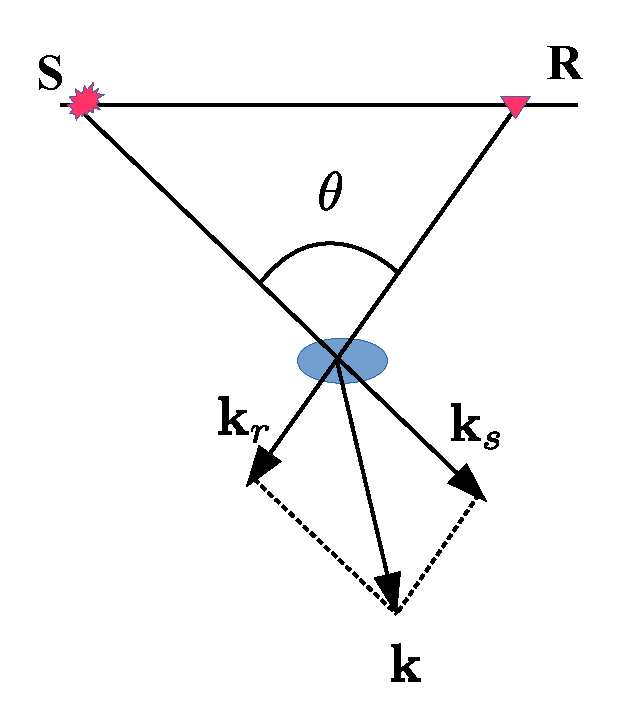
\includegraphics[width=0.40\textwidth]{Figure/chapter01/Wavenumbervector.pdf}}
   \caption{地下散射点处入射波矢量,散射波矢量以及散射角之间关系示意图。}
   \label{fig:WavenumberVector}
\end{figure}
\begin{figure}[b] 
   \centering 
   \subfloat{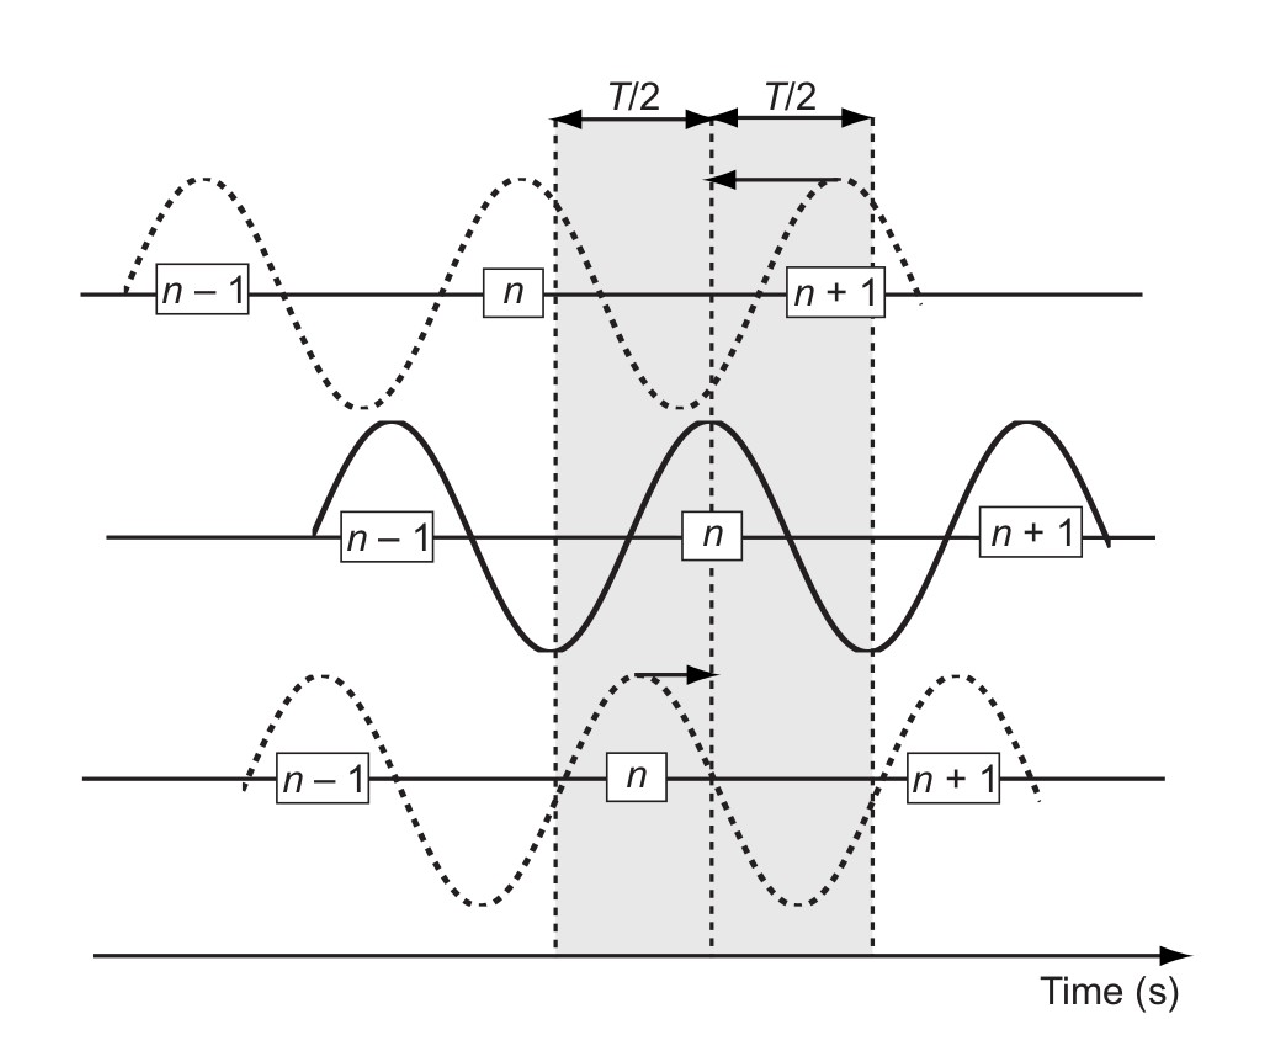
\includegraphics[width=0.60\textwidth]{Figure/chapter01/Cycle-skipping.pdf}}
   \caption{FWI波形匹配中的cycle-skipping现象(Virieux and Operto,
	   2009\cite{virieux2009overview})。当波形相差$T/2$周期以上的时候,数据将会在另一个周期中进行匹配,此时获得的数据残差会导致反演
   陷入局部极值。}
   \label{fig:Cycleskipping}
\end{figure}
因此,FWI的成功与否非常依赖于长偏移距记录和数据中有效的低频分量。如图\ref{fig:Cycleskipping}
所示,如果初始模型不够好导致波形匹配时相差$\frac{1}{2}$周期以上,那么就会使得反演陷入局部极值,这也就是所谓的“周波跳跃”问题。
在声波FWI中,人们发展了许多策略来应对非线性问题,如从低频到高频的多尺度策略(Sirgue and
Pratt, 2004\cite{sirgue.pratt:2004}; 刘国峰等, 2012\cite{刘国峰2012};
刘璐等,2013\cite{刘璐2013}; 曹书红和陈景波, 2014\cite{曹书红2014}; 
张文生等, 2015\cite{张文生2015}),根据时窗与偏移距分选数据子集逐步加入反演中(Shipp and
Singh, 2002\cite{shipp:2002}; Wang and Rao, 2009\cite{WangEtAl2009}; Sears et al., 2008\cite{sears2008}),
修正目标函数使其凸性更好(Luo and Schuster, 1991\cite{luo1991}; Tromp et al.,
2005\cite{tromp2005seismic}; Chi
et al., 2014\cite{ChiEtAl2014}; Wu et al., 2014\cite{Wu2014b}; Shin and Cha,
2008\cite{shin.cha:2008}; Luo et al., 2016\cite{Luo2016})等等。上述策略可以用
在EFWI中,但是由于更多参数的引入以及更复杂的弹性波波场,这些策略需要根据情况择优或者组合使用。

EFWI中不但会出现同样的强烈非线性,而且将面临更复杂的情况。
在构建初始模型的时候要同时获得足够好的$V_p$与$V_s$模型,才能对各种模式的转换波形进行
匹配。
与建立$V_p$模型不同,目前尚未有成熟流程来获得合理的S波速度模型。
许多EFWI方法在研究中都假设$V_s$与$V_p$之间有着固定的泊松比,因此可以通过简单的比例系数
来构建初始模型。但是当地下介质泊松比变化较大时很难获得较好的初始$V_s$模型。
此外,由于相同偏移距下,转换PS波的有效散射角范围相对PP波更小,并且S波速度相对较低等因素会导致EFWI对$V_s$高波数成分的过度更新,
这就又增加了EFWI的困难。
为了降低EFWI的非线性程度,许多学者通过
包络目标函数(Wu et al., 2014\cite{Wu2014b}; 黄超等,2015\cite{黄超2015};
王官超和杜启振,2016\cite{王官超2016}),
或者通过研究目标函数性态来指导多尺度策略的设计
(Brossier et al., 2010\cite{BrossierEtAl2010};王毓玮等,2016\cite{王毓玮2016})。
Tarantola(1986)\cite{tarantola:1986}指出EFWI应分主次顺序依次构建具有不同影响的参数。
也有学者多级地选取不同数据分量来进行多尺度反演(Sears et al., 2008\cite{sears2008}; Operto et al., 2013
\cite{operto2013guided})。然而实践中,诸多因素会制约这些策略的应用,例如低频缺失、初始模型不够好、子波估计困难、噪音干扰等。因此降低EFWI的非线性
程度使反演更加稳健可靠依然需要诸多努力。

2、多参数trade-off效应。如果物理模型中含有多个不同的物理参数,不同的参数扰动可能会引起相似的数据扰动。虽然产生的数据扰动可能不完全一致,
但是不同参数扰动产生的散射波场会在特定角度范围内重叠,这就导致常规的地面观测数据通常无法区分数据扰动来自哪一种
参数扰动,从而引起参数间的trade-off效应。这样的话,即使在初始模型足够好的时候也很难从数据扰动中恰当地恢复相应的参数扰动。

为了解决EFWI中的trade-off问题,
许多学者通过调查散射模式或者Hessian算子来选取不同的参数化方式(Wu and Aki, 1985\cite{wu.aki:1985}; Tarantola, 1986\cite{tarantola:1986}; 
Plessix and Cao, 2011\cite{plessix.cao:2011}; Gholami et al, 2013\cite{gholami2013})。
当然,最有效的就是考虑多参数Hessian算子,用Hessian的信息来压制trade-off的影响(Fichtner et al., 2001\cite{fichtner2011hessian}; Operto et al.,
2013\cite{operto2013guided}; Pan et al., 2015\cite{pan2015estimation}; Yang et al.,
2016\cite{Yang2016})。然而Hessian有关的计算所需代价太过昂贵,即使在声波FWI中也很难在大规模问题中获得应用。在EFWI中想要压制参数trade-off,就
需要在反演中利用Hessian非对角区块的信息。近期,在Hessian非对角区块的近似与利用方面,许多学者做出了一些有益的尝试,例如Wang
et al. (2016)\cite{WangYuweiEtAl2016}采用块对角Hessian压制参数耦合。Pan et
al (2017)\cite{PanEtAl2017}借助l-BFGS优化策略进行多参数反演。
Wang et al. (2015)\cite{wang:2015}和Ren and                                                                           
Liu
(2016)\cite{ren.liu:2016}初步讨论了基于弹性波模式解耦的梯度预条件方法及其在压制参数trade-off效应中的潜力。
Wang and Cheng (2017)\cite{WangEtAl2017}进一步对比了模式解耦与Gauss-Newton预条件梯度的差异,
指出模式解耦可以部分地利用Hessian非对角块来压制P波对$V_s$反演的干扰。由于常规地震观测很难敏感地捕捉密度信息,至今密度
的反演依然非常困难(Jeong et al., 2012\cite{jeong2012full}; Prieux et al., 2013\cite{prieux:2013a}; Yang
et al., 2016\cite{Yang2016})。
\subsection{弹性反射波波形反演研究现状}
常规FWI在长偏移距、宽方位数据中有着不错的效果,但主要是利用了透射波以及临界反射波所携带的信息来更新速度模型的
中低波数分量。由于FWI的成功非常依赖这些波场信息,使得地震数据往往缺乏足够的大偏移距信息来更新中深部结构的中低波数成分。
换句话说,在中深部区域,FWI往往过多地更新来自反射数据的高波数成分(相当于最小平方偏移)。从式\eqref{eq:Modelwnb}
可以看出,在相同频率和速度情况下,深部的反演需要更大的角度孔径才能确保足够的低波数照明,这也意味着要更大的偏移距。然而,即使
采用现有宽方位、长偏移距观测也很难保证这样的覆盖,而且更长的偏移距也意味着更强的非线性\cite{sirgue2006importance,virieux2009overview}。

利用反射波信息可以更好地照明深部结构。通常,可以在成像域或者数据域实现基于深部反射波的速度更新。在成像域,该类方法通常被称为偏移速度分析(MVA),主要利用拉平
共成像点道集作为收敛准则。
在实际生产中,通过反射走时层析来反演反中深部的背景速度已经是非常成熟的技术(Woodward,
1992\cite{Woodward1992}; Meng et al., 2004\cite{MengEtAl2004}; Woodward et al., 2008\cite{
Woodward2008}; Jones, 2010\cite{Jones2010})。
它通过将共成像点道集上的剩余时差(或深度差)反投影到射线或Born波路径上来更新速度。不过基于射线理论的走时层析经常需要进行一些人工拾取,比如在每轮迭代中进行
成像剖面与成像道集剩余曲率的拾取。在构造复杂区域,高频渐近假设失效,使得射线走时层析的有效性明显下降。
基于波动理论的WEMVA可以很好地应对上述问题,但是通常
需要借助昂贵的扩展域成像,通过最小化非零偏移距的能量来实现模型更新,如Sava and
Fomel (2006)\cite{SavaEtAl2006}; Yang and Sava(2011)\cite{YangEtAl2011}; Almomin and
Biondi(2012)\cite{Almomin2012}; Sun and Symes(2012)\cite{SunEtAl2012}。尽管WEMVA在
二维应用中取得了不错的效果,但三维应用中过高的计算成本是一个明显的制约因素。
%一方面偏移成像需要大量计算,
%另一方面扩展成像条件的施加同样耗费极大。
针对反射走时,Luo et
al. (2016)\cite{Luo2016}用时间轴方向的扩展成像与Rytov近似结合,提出了全走时反演(FTI)方法并在理论合成数据上
获得了不错的反演效果。该方法实质上也是一种成像域的速度反演方法。

在数据域同样可以利用反射波对模型深部进行更新。
有些学者(Chavent et al., 1994\cite{ChaventEtAl1994}; Plessix et al., 1998\cite{PlessixEtAl1998}; Clment et al., 2001\cite{ClementEtAl2001})
将速度模型分成高波数(反射率)与低波数(背景模型)成分,提出了偏移成像走时层析(MBTT)方法。
从Alder (2008)\cite{Adler2008}提出的基于射线理论的非线性层析方法出发,Wang
et al. (2014)\cite{WangEtAl2014}和Yang et al.
(2016)\cite{YangEtAl2016}采用一次偏移后拾取+图偏移的方式建立叠前数据的不变量(如走时,出射慢度等),
通过对
叠前数据不变量的多次拟合来更新层析速度模型,既减少了人工拾取,又达到加快收敛的效果。

基于波动理论的数据域速度反演近年来受到了广泛的关注。
受MBTT方法的启发,Xu et al. (2012)\cite{xu:2012}提出了反射波波形反演(RWI)方法。它先采用RTM或LSRTM获取反射率模型,
然后用Born模拟(反偏移)来预测反射率所产生的反射波。反射波与背景波场的互相关可以得到反射波波路径(敏感核函数)信息。
RWI的关键就是将数据残差反投影到反射波波路径上,从而更新模型分量的中低波数成分。
RWI方法出现后,许多学者做了大量研究,采用了波形拟合的$L_2$范数,如Xu
et al. (2012)\cite{xu:2012}, Wang et al. (2013)\cite{Wang2013}, Wu and
Alkhalifah (2015)\cite{Wu2015b},
Zhou et
al. (2015)\cite{zhou:2015}。
近期,Irabor and
Warner (2016)\cite{Irabor2016}和Wang et al.
(2016)\cite{WangFangEtAl2016}通过上、下行波分离来帮助常规FWI获取背景分量的更新,其实质也利用了反射波波路径的信息。
%然而,尽管RWI的目的在于更新背景速度,波形拟合的$L_2$范数在背景速度与真实值相差较远的时候,反偏移
%所预测的与
然而,尽管RWI的目的在于更新背景速度,当背景速度与真实值相差较远的时候,反偏移
所预测的与观测数据中的反射波波形也可能相差半个周期以上,从而导致波形拟合的$L_2$范数产生周波跳跃。Wang et
al
(2013)\cite{Wang2013}指出采用低频数据可以一定程度上缓解跳周现象。为了避免振幅相关的目标函数带来的非线性,更趋于线性关系的
走时类目标函数获得了关注。Ma and
Hale
(2013)\cite{ma2013}采用动态图像识别(DIW)来获得模拟与观测反射数据之间的时移量,从而提出了波动方程反射走时反演(WERTI)方法。类似的,Chi
et al. (2015)\cite{chi2015}和Wang et al.
(2015)\cite{Wang2015}采用互相关类的方法来获取模拟与观测反射数据同相轴的时移(或空移)量。
以上有关RWI的研究都是基于声波方程的。

在弹性反射波反演研究中,目前只有Guo and
Alkhalifah (2016)\cite{Guo2016}将Wu and
Alkhalifah (2015)\cite{Wu2015b}的声波RWI思路进行了扩展。
对于弹性反射波形反演(ERWI),除了声波RWI中面临的问题,还需要处理更多的复杂情况,如多参数trade-off、模式转换、更复杂的反射记录以及
$V_s$反演的困难等。为了应对这些问题,
%利用波模式解耦来分别获取P与S反射波然后应用到RWI或反射走时反演(RTI)中将是非常直观的思路,
本文第四章将论述怎样借助弹性波模式解耦与多分量记录P/S分离来建立比较有效的ERWI方法与流程。
%考虑到弹性波的哪些特殊情况,以便获得可行的ERWI方案。
%许多研究通过选取不同的目标函数来选取方法对应不同名称的反演方法,但核心思想都是一致的

\subsection{弹性波最小平方逆时偏移研究现状}

目前有许多成像方法,如Kirchhoff偏移、高斯束偏移和逆时偏移(RTM)等可以用来恢复地下界面结构形态。
但是随着需求的变化与技术的进步,构造信息已经不能满足勘探的需要。人们想要
获得更高分辨率的弹性参数以便直接或间接用于岩性/流体区分等更高级的任务。
常规FWI算法可以用于参数模型的高分辨率成像(反演),但是会受到许多因素困扰,
如初始模型不好或者数据低频缺失导致的cycle-skipping问题、地震子波未知、正演算子不准确等等。
而且,常规FWI一般需要从低频到高频逐步恢复连续的波数谱。如果单纯想获得模型高波数成分,
用FWI方法就太过复杂或困难。除FWI之外,通常也会通过最小平方偏移(LSM)来实现高波数成分的重构。
早期,Beylkin
et al. (1985)\cite{BeylkinEtAl1985}和
Bleistein (1987)\cite{Bleistein1987}等学者通过广义Radon变换来导出Kirchhoff成像中的振幅校正因子,实现所谓的真振幅成像。
该方法通过射线理论计算Green函数,正问题采用Born近似
,可快速地迭代求解反问题。
针对Kirchhoff偏移,Schuster(1993)\cite{Schuster1993}提出了应用于井间数据的LSM算法,而后Nemeth et al.
(1999)\cite{Nemeth1999}将该方法应用到了地面数据中。

以波动方程为引擎的最小平方逆时偏移(LSRTM)近年来一直是研究的热点,
尽管其计算代价昂贵,但可以处理复杂非均匀介质中所产生的多路径问题。
LSRTM通常可认为是线性的全波形反演。线性近似下若能获得Hessian矩阵的逆算子就可以通过施加逆算子快速获得反问题的解。
但是Hessian的计算与求逆在实际问题中非常困难,
故在空间域采用Hessian的近似来校正成像结果是一种快速实现LSRTM的方法(Chavent and Plessix, 
1999\cite{ChaventEtAl1999}; Shin et al., 2001\cite{shin2001improved}; Symes,
2008\cite{Symes2008})。然而,这种方法在复杂介质中并
不总是有效。另外一种方式是通过在数据域求解目标函数的最小化问题。
假设在已经获得足够好的低波数模型成分之后恢复模型的高频扰动,即获得“像”或
反射率,使得在最小平方意义下,用该反射率所预测的反射数据能与观测数据达到最佳匹配。
这一过程与在单次迭代中通过计算二阶伴随状态方程实现基于
Gauss-Newton法(Bae et al., 2012\cite{bae2012frequency}; Metiver et al.,
2014\cite{Metivier2014})的FWI是一致的。
因此,最小平方逆时偏移与全波形反演的理论框架基本是一致的,只是输入数据(反射波/全波场)和输出结果(高频扰动/模型参数)不一样。
因此目前LSRTM研究中主要通过最小化Born模拟的反射数据与观测数据之间的残差来改善成像质量,获得更高分辨率的反射率、波阻抗
界面或弹性参数扰动的反演结果(Dai and
Schuster, 2013\cite{Dai2013}; Dong et al., 2012\cite{Dong2012}; Luo and
Hale, 2014\cite{Luo2014})。

许多学者针对LSRTM中的其他问题也做了大量的研究工作。Wong et al.
(2015)\cite{WongEtAl2015}将自由表面多次波加入到成像条件中,进而增加地下照明。Zhang et al.
(2015)\cite{ZhangEtAl2015}选取零延迟互相关目标函数来减弱子波估计不准以及振幅描述不准带来的非线性。刘玉金和李振春
(2015)\cite{刘玉金2015}基于成像域的速度反演方法(Symes, 2008\cite{Symes2008a})
在扩展域进行LSRTM,在速度不准确的情况下仍然可以得到合理的成像结果。
近期,为了更准确地描述波传播过程,同时获得更多的参数成像,原本基于常密度声波方程的
LSRTM被推广到了变密度声波介质(Yang et al, 2016)\cite{Yang2016}、衰减介质(Dutta and
Schuster, 2014\cite{DuttaEtAl2014}; 李振春等,2014\cite{李振春2014}; Dai et al.,
2015\cite{Dai2015})以及弹性介质中(Duan et al., 2016\cite{Duan2016}; Feng and Schuster,
2016\cite{Feng2016}; Xu et al., 2016\cite{Xu2016}; Ren et al., 2016\cite{RenEtAl2016})。

相比声波成像,弹性波成像可以提供更多的地下信息,例如转换横波成像可改善气云区成像,有助于区分岩性和识别流体。
但是,许多问题会很大程度上影响弹性波成像质量。
首先,传统声波成像方法中观测孔径限制、粗网格采样、低频噪音以及数据缺失引起的偏移假象同样会出现在弹性波成像中;
其次,记录中的P与S波数据很难完全区分开,泄漏的波模式会引起假象,即“cross-talk”;
再次,一般的成像条件会导致转换波图像的极性反转问题,因此需要选取合适的校正方法(Du et al,
2014\cite{DuEtAl2014}; Gong et al, 2016\cite{GongEtAl2016}; Rocha et al,2016\cite{RochaEtAl2016a})。
%常规ELSRTM可以较好的压制由于观测和数据不完备造成的成像噪音,同时对cross-talk也有一定的压制作用。
%为了解决
%波模式完全区分开,因此其中某些波模式的会因速度不对而被错误地成像。这些非物理的模式就会引起假象,也即“cross-talk”。
%而通过ELSRTM则可以提高成像的分辨率,并且可以压制由于观测孔径限制,粗网格采样以及数据缺失引起的偏移假象。
%弹性波成像需要处理矢量波的问题,也就需要选取合适的成像条件(Du et al, 2014\cite{DuEtAl2014};Gong et
%al, 2016\cite{GongEtAl2016};Rocha et al,2016\cite{RochaEtAl2016a}),
近期Wang et al(2016)\cite{WangChenlongEtAl2016}面向各向同性与横向各向同性(TI)介质提出了
更具有物理含义的无极性反转的矢量成像条件。
最近,从EFWI理论框架出发,有学者(如Duan et al., 2016\cite{Duan2016}; Feng et al., 2016\cite{Feng2016} 等)
推导出了与EFWI梯度非常类似的成像条件,可以回避极性反转问题。
基于第二章对EFWI算法的分析,模式解耦带来的好处同样能在ELSRTM中发挥作用,尤其是压制传统弹性波成像中模式串扰引起的假象。


\section{研究内容}
基于多分量地震数据重构弹性参数模型是本文的重点。
除了层析成像与WEMVA方法之外,目前主流的模型参数估计方法包括FWI、RWI和LSRTM。
我们将以上三种方法扩展到弹性介质,采用EFWI构建高分辨率弹性参数模型,采用EWERTI通过弹性波走时信息构建中深部的背景弹性波速度,
而在可靠的初始弹性速度模型基础上采用ELSRTM构建模型的高波数成分(反射界面的高分辨率图像)。
整个论文中,弹性波模式解耦将是其中最核心的方法,为不同分辨率的弹性参数反演提供解耦的P与S波数据子集,
从而降低反问题的非线性程度、压制参数间trade-off效应。
%以利用由此带来的降低参数间trade-off的便利。
本文下面几章将分为以下四个部分来详细展开:

第二章将通过模式解耦对EFWI梯度进行预条件,降低反演过程中的参数trade-off程度,并达到加速收敛的效果。
首先,通过弹性波Born近似,分析$V_p$与$V_s$扰动的
辐射模式,并给出解耦的Frech{$\acute{e}$}t导数(Jacobian矩阵)。然后,调查解耦后的P波与S波数据对梯度的贡献并提出在梯度计算中的交叉项近似。
在此基础上,通过伴随状态法快速计算得到预条件的梯度,
即正传波场与解耦后反传波场的零延迟互相关。
然后,为了获得更多物理机制上的认识,将计算并分析基于解耦的Hessian和分辨率矩阵,同时也对比模式解耦预条件的梯度与Gauss-Newton(GN)梯度的异同。
接着,利用流体饱和砂岩模型以及Marmousi-II模型的数值算例验证基于模式解耦的EFWI的有效性。
最后,将讨论引入密度给反演带来的复杂性以及模式解耦EFWI的表现。

第三章将通过弹性波波动方程反射走时反演(EWERTI)来重建速度模型中深部的中低波数分量。
文中采用反射波走时拟合差作为目标函数进行反演,其中的走时残差将通过DIW方法来获取。
沿用RWI的思路,通过Born模拟来构建反射波关于背景速度的核函数,即反射波波路径。
参照Ma and Hale (2013)\cite{ma2013}的方式,推导出弹性波反射走时反演的伴随震源与梯度。
通过目标函数的性态分析调查EWERTI的稳健性与收敛性。然后基于反射核函数观察不同反射波波模式对反射波路径的影响。
为了克服反演中的非线性以及P波与S波速度之间的trade-off,将分两个阶段来分别恢复$V_p$与$V_s$:首先,采用PP波反射走时来重建$V_p$背景模型;
然后,在获得足够好的背景$V_p$后,再采用分离出的PS波反射走时重构$V_s$背景模型。
在此过程中,本文提出用地面多分量数据P/S分离来帮助获取PP或PS的走时残差,用空间波场模式解耦来预条件目标函数关于$V_p$或$V_s$的梯度。
最后将在Sigsbee2A模型上进行算法验证。

第四章将采用ELSRTM来获取弹性参数模型的高波数分量。首先,从反演框架出发,建立Born模拟与观测反射数据之间的最小二乘拟合目标函数,
利用矩阵形式的弹性波方程通过拉格朗日乘子法获得伴随状态方程,并导出ELSRTM的梯度公式。
之后根据第二章的推导,利用波模式解耦对梯度进行预条件处理。
由于不同模型的参数耦合程度不同,将根据具体情况设计不同的反演策略。简单模型和Marmousi-II模型的数值实验将用来验证
策略的有效性。
此外,由于ELSRTM基于Born近似,Born正演数据与反射数据之间存在差异。文中也对比了采用Born模拟数据与反射数据反演结果的差异。
%LSRTM为线性FWI过程,反问题的复杂程度将大为降低,
%此外,根据不同模型的trade-off程度设计不同的反演策略,并将对比这些策略在解决参数耦合问题的效果。
%简单模型与Marmousi的数值实验将用来验证算法的有效性。

第五章将对本文的工作进行总结,指出论文的创新与不足之处,并给出下一步的研究计划。

%
%%% Local Variables:
%%% mode: latex
%%% TeX-master: t
%%% End:



\chapter{弹性波模式解耦全波形反演}
\label{cha:MD-EFWI}
\section{引言}
针对地下介质的定量成像方法对于定位与刻画油气储层、监测CO$_2$注入以及估计近地表土壤和岩石的物理性
质非常重要。相比于从地震偏移获得的定性化的成像剖面,人们更希望得到定量化的地下弹
性参数。地震反演旨在采用迭代优化类方法通过拟合正演数据与实际观测数据来恢复地下弹性参数模型。
相比走时层析类方法,
%例如Luo and Schuster (1991)\citep{luo1991},
FWI提供
了更加完善的理论,同时利用走时与振幅信息来反演介质参数\cite[]{tarantola:1986}。
随着长偏移距、宽方位和宽频带采集技术的应用,全波形反演已经成为构建高质量速度模型和进行定量地震成像的有效工具\cite{virieux2009overview}。

然而,FWI有许多制约因素。首先,它所需的计算量十分巨大,尤其是在三维模型反演中。尽管梯度类的局部优化方法并不能保证反演收敛到全局最优解,
但为了降低计算代价仍然被广泛应用于FWI中。收敛性更好的基于Hessian的反演方法\cite{mora:1987,crase1990robust}
因其更昂贵的计算代价则在大多数FWI应用中被舍弃不用。此外,为了减少计算量,人们通常采用声学近似来反演获得P波速度\cite{ravaut2004multiscale,operto2006crustal}。
但实际中,即使是以P波为主的单分量地震数据,声学近似也只能保证运动学信息的准确,振幅的可靠性只有在小角度入射时才有保证。
这也是声波FWI通常需要非常仔细的数据预处理和预条件的主要原因。总之,地震数据中总是包含弹性波场,即使在海洋勘探中,
声波反演也不能考虑到由于模式转换带来的能量损失,会对声波数据过度拟合而低估模型中界面周围的速度反差。

弹性波全波形反演(EFWI)能够从多分量数据中估计地下介质的弹性参数,如$V_p$, $V_s$和$\rho$。
%尽管其仍然需要很大计算代价,EFWI还是在很多实际数据中获得了应用
%\cite{crase1992nonlinear,djikpesse.tarantola:1999,sears2008,sears:2010,prieux:2013a,prieux:2013b,vigh:2014}。
%其实现方式可以在时间域\cite{shipp:2002},可以在频率域\cite{brossier2009},也可以采用混合的方式在时间域进行正演模拟而在频率域求解
%\cite{nihei.li:2007,sirgue:2008}。
然而,EFWI中多个参数参与反演会增加反问题的非线性程度,也会受到由于不同物理参数之间串扰(trade-off)
的影响\cite{forgues.lambare:1997}。
%在海洋环境中,尤其是在软海底环境中,由于PS的转换模式非常弱,
%基于拖缆或者海底多分量数据的EFWI的非线性程度会变得更严重\cite{sears2008}。
当$V_p$,$V_s$和$\rho$在结构上有差异时,trade-off效应会更加明显。
将声波FWI扩展到弹性介质中需要付出更多的努力。
很多学者指出参数化方式对缓解trade-off效应非常重要,可以通过调查散射模式或者Hessian算子来选取恰当的参数化方式
\cite[]{wu.aki:1985,tarantola:1986,plessix.cao:2011,gholami2013}。
%另外一个常用的降低非线性程度的方法是
%将速度扰动分解为低波数与高波数成分,然后用不同的数据子集多尺度地进行反演\cite[]{symes.carazzone:1991,bunks1995multiscale,clement:2001,shin.cha:2008,dehoop:2012,
%xu:2012,biondi.almomin:2013,ma2013,warner2016adaptive,alkhalifah2015scattering}。
Tarantola(1986)\cite{tarantola:1986}指出可先重构出对数据具有主要影响
的参数,再重构出对数据有次级影响的参数。Sears(2008)\cite{sears2008}提出了一个有效的多尺度策略,通过时间窗来选取海底电缆(OBC)
数据中的不同子集进行多尺度反演。Operto(2013)\cite{operto2013guided}讨论了如何多级地选取不同的数据分量以及不同的参数类型进行反演,从而
压制trade-off效应并降低反演的非线性程度。Xu and McMechan\cite{xu.mcmechan:2014}提出了一个多步长的策略来提高密度模型的反演精度。

%另一个行之有效解决trade-off的方法就是在反演中施加Hessian算子。
Hessian逆的对角块能够消除几何扩散以及带限效应带来的模糊性,而非对角块能够压制
trade-off效应\cite[]{pratt1998gauss,fichtner2011hessian,operto2013guided,innanen2014seismic,pan2015estimation}。
对于大规模问题,为了避免不可承受的Hessian计算及求逆,很多研究工作都旨在寻找对Hessian逆的有效近似,例如采用拟Hessian\cite[]{shin2001improved,choi.shin:2008}
或者通过拟牛顿方式迭代构建Hessian的向量乘,如L-BFGS方法\cite[]{nocedal2006numerical,brossier2009}。
Sheen et al(2006)\cite{sheen:2006}通过互易原理和褶积定理来计算近似Hessian从而实现了时间域基于GN的EFWI方法。
Bae et al(2012)\cite{bae:2012}提出了频率域基于GN共轭梯度法的声弹耦合FWI。
Pratt et al(1998)\cite{pratt1998gauss}采用“虚震源”引起的偏导数波场的概念解释了梯度与Hessian算子的物理含义。参数耦合效应是由于
不同参数的偏导数波场在特定角度范围内的重叠导致的。因此,Wang et al (2015)\cite{wang:2015}发现通过解耦弹性波场并在不同阶段分别选取P波与S波
数据来反演不同参数有助于压制trade-off效应。%通过调查解耦之后的P波与S波目标函数,Ren and Liu (2016)\cite{ren.liu:2016}证明了波场的解耦可以降低EFWI的非线性程度。
此外,模式解耦也是弹性波逆时偏移中获得具有物理含义成像的关键步骤\cite{yan:2008,wang2016scalar}。

本文EFWI方法中不是经验性地解耦正、反传波场以及地震记录\cite{ren.liu:2016}来计算梯度,而是采用了更有物理意义同时节省计算量的预条件方式,
即在计算梯度时只解耦反传波场。通过调查解耦后的Frech{$\acute{e}$}t导数、
Hessian矩阵以及分辨率矩阵等反演中的关键要素,来解释模式解耦预条件的梯度相比常规预条件梯度能够更好压制参数trade-off的理论机制。
为了简单起见,我们先抛开密度,只在讨论部分涉及包含密度的三参数反演问题。
%首先,通过弹性波Born近似,我们分析了P波速度与S波速度扰动的
%辐射模式,并导出了解耦的Frech{$\acute{e}$}t导数或Jacobian矩阵;然后,我们调查了解耦后的P波与S波数据对梯度的贡献并提出了在梯度计算中的交叉项近似。
%在此基础上,预条件的梯度可以通过伴随状态法\cite[]{plessix2006}快速有效地计算得到,也即正传波场与解耦后反传波场的零延迟互相关。
%然后,为了获得更多物理机制上的认识,我们计算并分析了基于解耦的Hessian和分辨率矩阵,同时也比较了MD预条件后的梯度与GN梯度的异同。
此后,通过在流体饱和砂岩模型以及Marmousi-II模型的数值算例验证模式解耦EFWI的有效性。
最后,将讨论密度参数对反演带来的复杂性以及模式解耦预条件共轭梯度(MDPCG)算法对三参数EFWI的贡献,并给出本章结论。
%\clearpage

\section{弹性波正问题}
\label{sec:forward_problem}
如果视地球内部介质为弹性介质,则地震波场在地下传播的控制方程可写为:
\begin{equation}
	\rho \frac{\partial u^2_i}{\partial t^2}  -
	\frac{\partial}{\partial x_j}\left[c_{ijkl}\frac{\partial u_{k}}{\partial
	x_l}\right]=f_i,
	\label{eq:WE} 
\end{equation}
其中$u_i$和$f_i$ 分别为质点位移矢量以及体力震源项的第$i$分量,$\rho$为密度,$c_{ijkl}$
为刚度矩阵张量的分量。公式中所有的下标取值为从1到3。重复下标涉及默认的Einstein求和方式。
对于各向同性介质,刚度矩阵张量满足:
\begin{equation}
	c_{ijkl}=\lambda\delta_{ij}\delta
	_{kl}+\mu(\delta_{ik}\delta _{jl}+\delta _{il}\delta_{jk}),
	\label{Lame}
\end{equation}
其中$\lambda$和$\mu$为Lam$\acute{e}$系数,$\delta_{ij}$为Kronecker函数。 

根据Born近似,在$\mathbf{x}$ 位置上对刚度系数做一个微小扰动,$\delta
c_{ijkl}(\mathbf{x})$,将会产生一个扰动波场$\delta \mathbf{u}$,满足:
\begin{equation}
	\rho \frac{\partial \delta u^2_i}{\partial t^2}  -
	\frac{\partial}{\partial x_j}\left[c^0_{ijkl}\frac{\partial \delta u_{k}}{\partial
	x_l}\right]=\frac{\partial}{\partial
	x_j}\left[\delta c_{ijkl}\frac{\partial
	u^0_{k}}{\partial x_l}\right],
	\label{eq:BornApp}
\end{equation}
其中,$\mathbf{u}^0$为在背景介质$c^0_{ijkl}$中满足方程\eqref{eq:WE}
的背景场。上式说明扰动场$\delta \mathbf{u}$可看作是入射波场$\mathbf{u}^0$与参数扰动$\delta
c_{ijkl}(\mathbf{x})$相互作用产生的次级源所引发。为了简单起见,本章的公式推导主要在频率域进行,但是大部分的计算操作(尤其是波场延拓)则在时间域实现。
利用表示定理与散度定理(Kamath and Tsvankin, 2016)\cite{kamath2016elastic},扰动波场满足:
\begin{equation}
	\delta u_n(\mathbf{r},\omega)=-\int_{\Omega(\mathbf{x})}{\frac{\partial
	u^0_{k}(\mathbf{x},\omega)}{\partial x_l}
	\frac{\partial G_{ni}(\mathbf{r},\mathbf{x},\omega)}{\partial
	x_j} \delta
	c_{ijkl}(\mathbf{x})}
	d\Omega(\mathbf{x}), \quad (n=1,2,3),
	\label{eq:Repre}
\end{equation}
其中,$\omega$表示频率,$G_{ni}(\mathbf{r},\mathbf{x},\omega)$为弹性波背景格林函数,表示在$\mathbf{x}$处沿$i$方向的单位体力源
所产生的在$\mathbf{r}$处沿$n$方向的质点位移,$\Omega(\mathbf{x})$为体积积分范围。注意方程\eqref{eq:Repre}只考虑了一阶散射的情况。
刚度系数扰动与速度扰动之间的关系为:
\begin{equation}
        \delta c_{ijkl}=\frac{\partial c_{ijkl}}{\partial V_p}\delta V_p
        +\frac{\partial c_{ijkl}}{\partial V_s}\delta V_s,
        \label{eq:deltaLame}
\end{equation}
以及
\begin{equation}
        \begin{split}
                &\frac{\partial c_{ijkl}}{\partial V_p}=2\rho V_p\delta_{ij}\delta_{kl},\\
                &\frac{\partial c_{ijkl}}{\partial V_s}=2\rho
                V_s(-2\delta_{ij}\delta_{kl}+\delta_{ik}\delta _{jl}+\delta_{il}\delta_{jk}),
        \end{split}
        \label{eq:deltaLame_vel}
\end{equation}
将方程\eqref{eq:Repre}重写为速度参数化方式:
\begin{equation}
        \delta
        u_n(\mathbf{r},\omega)=\int_{\Omega(\mathbf{x})}{\left[J_{n,V_p}(\mathbf{r,x},\omega)\delta
                V_p(\mathbf{x}) +J_{n,V_s}(\mathbf{r,x},\omega)\delta
        V_s(\mathbf{x})\right]
                }
                d\Omega(\mathbf{x}),
        \label{eq:SplitRepre}
\end{equation}
其中
\begin{equation}
        J_{n,M}(\mathbf{r,x},\omega)=
        T_{ij,M}(\mathbf{x},\omega)G_{ni,j}(\mathbf{r,x},\omega), \quad M\in\{V_p,V_s\},
\label{eq:KernelAB}
\end{equation}
并且
\begin{equation}
\begin{split}
                &T_{ij,M}(\mathbf{x},\omega)=\frac{\partial c_{ijkl}}{\partial M}\frac{\partial
                        u^0_{k}(\mathbf{x},\omega)}{\partial x_l},\\ 
                        &G_{ni,j}(\mathbf{r,x},\omega)=\frac{\partial
                                G_{ni}(\mathbf{r},\mathbf{x},\omega)}{\partial x_j},
\end{split}
\label{eq:traction}
\end{equation}
式\eqref{eq:KernelAB}中$J_{n,M}$表示速度扰动对应的偏导数波场\cite[]{pratt1998gauss},$T_{ij,M}$
表示背景波场$\mathbf{u}^0$与速度扰动$\delta V_p$ (或 $\delta V_s$)
作用产生的次级震源,$G_{ni,j}$表示格林函数的空间导数。假设模型网格数与接收点个数为L和K,则方程\eqref{eq:KernelAB}可以重写为离散的形式:
\begin{equation}
        \mathbf{J}_{n,M}(\mathbf{x}_l,\mathbf{r}_k)=
        (\mathbf{T}_M(\mathbf{x}_l):\mathbf{G}'(\mathbf{x}_l,\mathbf{r}_k))_n,\quad
        k=1,2,...,K;\quad l=1, 2,...,L,
        \label{eq:EquivFre}
\end{equation}
其中的双点符号$:$代表了以下操作:
\begin{equation}
    (\mathbf{T}_M:\mathbf{G}')_{n}=\sum_{i,j=1}^{3}T_{ij,M}G_{ni,j}.
    \label{eq:contraction}
\end{equation}
为了简化表达多分量数据,我们隐藏下标$n$。因此,方程\eqref{eq:SplitRepre}可写成矩阵形式:
\begin{equation}
            \begin{pmatrix}
                        \mathbf{J}_{V_p}&\quad\mathbf{J}_{V_s}
    \end{pmatrix}
    \begin{pmatrix}
       \delta  \mathbf{V}_p\\
       \delta \mathbf{V}_s
    \end{pmatrix}
    =
        \mathbf{\delta u},
        \label{eq:finalMatrix}
\end{equation}
其中$\mathbf{J}_{V_p}$和$\mathbf{J}_{V_s}$为$K\times L$大小的Frech{$\acute{e}$}t导数(Jacobian)矩阵,
$\delta \mathbf{V}_p$和$\delta \mathbf{V}_s$为长度是$L$的模型参数向量,$\delta \mathbf{u}$为在接收点位置上的弹性散射波场。
方程\eqref{eq:finalMatrix}可以进一步简写为:
\begin{equation}
        \mathbf{J}\delta \mathbf{m}
    =
        \mathbf{\delta u},
        \label{eq:finalMatrixshort}
\end{equation}
其中$\mathbf{J}=(\mathbf{J}_{V_p}\quad\mathbf{J}_{V_s})$,且 
$\delta \mathbf{m}=(\delta\mathbf{V}_p \quad \delta\mathbf{V}_s)^T$.

\subsection{P/S波数据耦合与辐射模型}
方程\eqref{eq:finalMatrix}或\eqref{eq:finalMatrixshort}表明Jacobian矩阵与参数扰动向量的乘积即为相应的散射数据响应,所有响应的
叠加就组成了整个散射波场。从图\ref{fig:radiationpattern}中展示的散射模式可看出,$\delta V_p$只通过PP模式散射P波数据,而$\delta V_s$
则散射所有模式的P波和S波数据。这就很难分辨出散射数据中的P波是来自于哪一类速度扰动($\delta V_p$或$\delta V_s$)。
幸运的是,散射S波仅仅由$\delta V_s$产生,因而对于单次散射的弹性波数据来讲,耦合效应只会出现在P波模式中。
既然反演中的参数耦合效应是由于不同模型参数的偏导数波场在特定角度范围内的重叠导致的\cite{tarantola:1986,operto2013guided},
所以很自然地,本文提出采用模式解耦来作为降低EFWI参数耦合效应的方法。
\begin{figure}[!htb]
    \begin{center}
        \subfloat[]{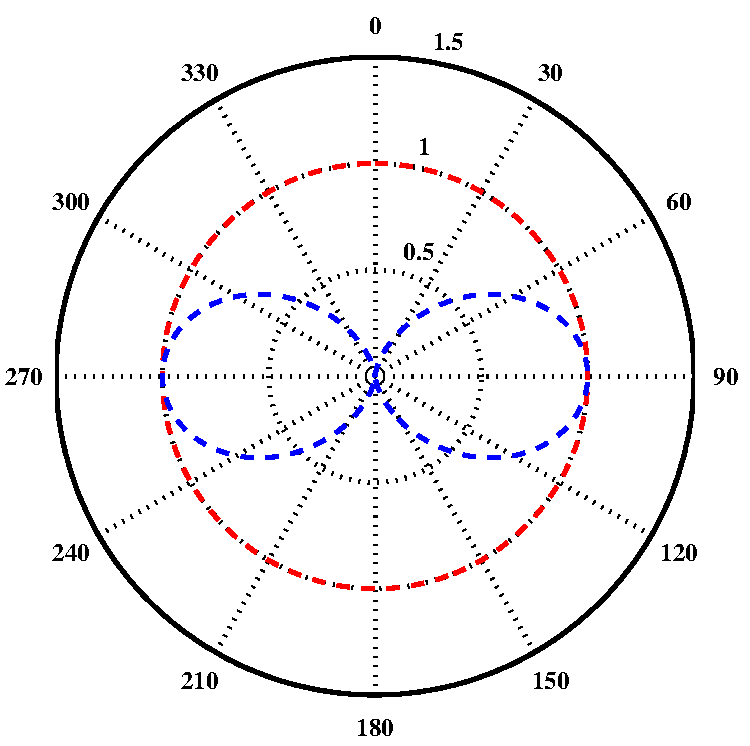
\includegraphics[width=5cm]{Figure/chapter02/radiationpattern/Fig/PP.pdf}}
%        \subfloat{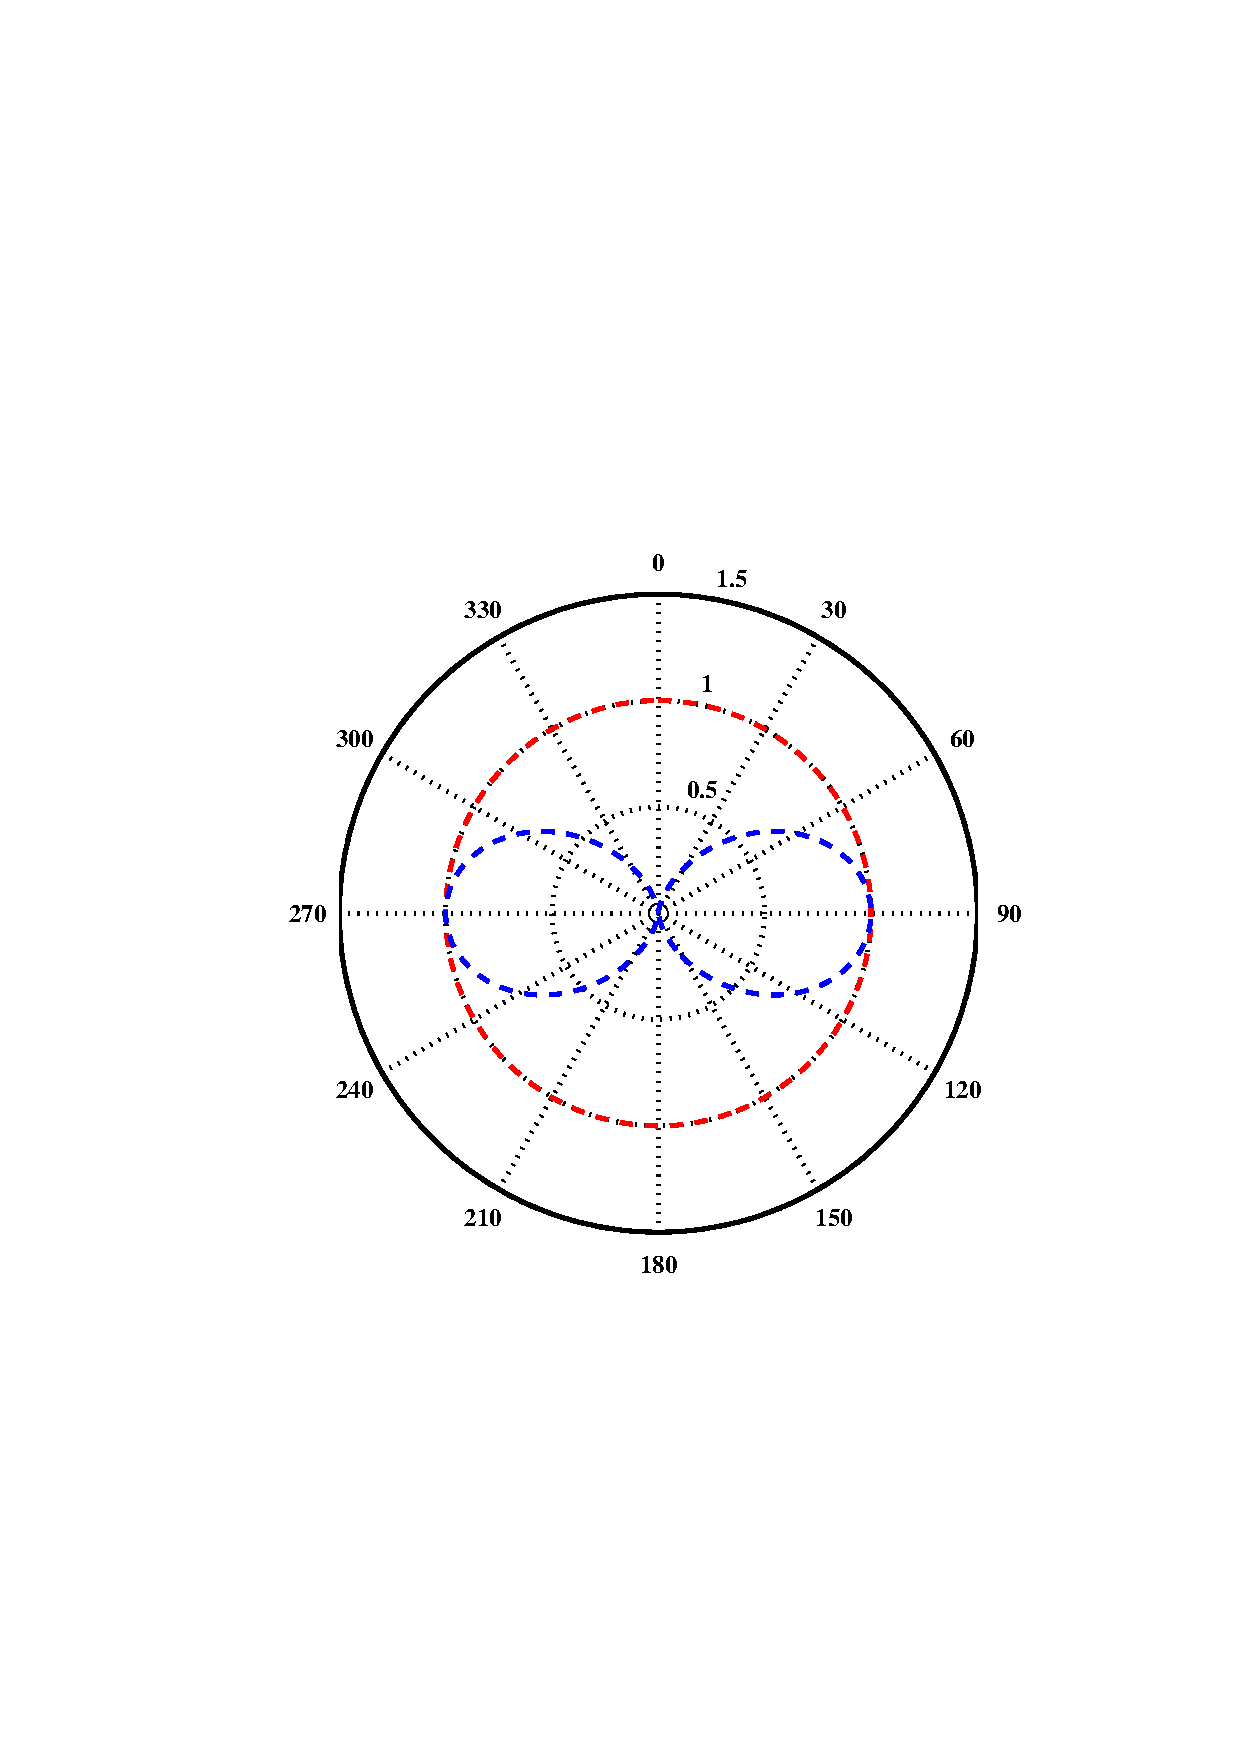
\includegraphics[width=5cm]{radiationpattern/Fig/PP.pdf}}
        \subfloat[]{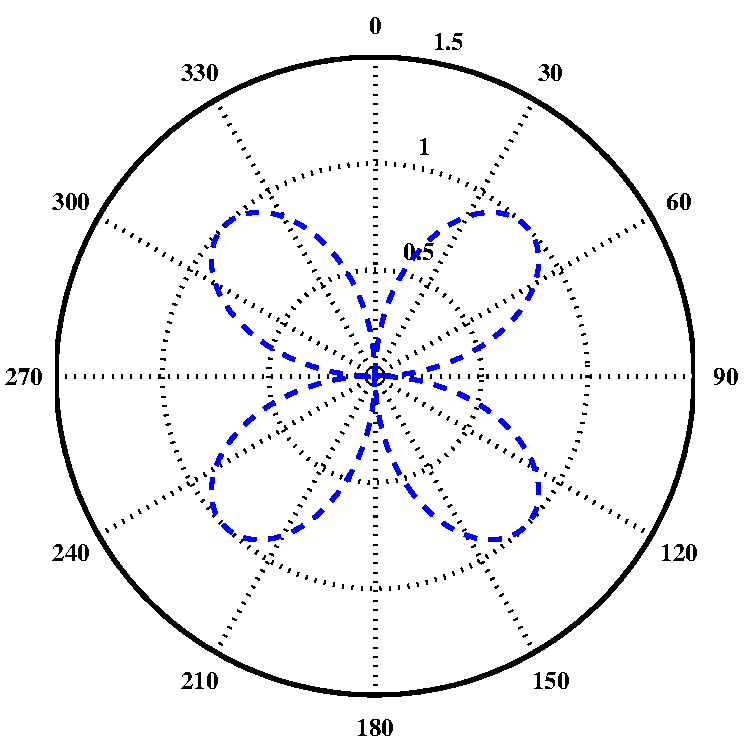
\includegraphics[width=5cm]{Figure/chapter02/radiationpattern/Fig/PS.pdf}}\\
        \subfloat[]{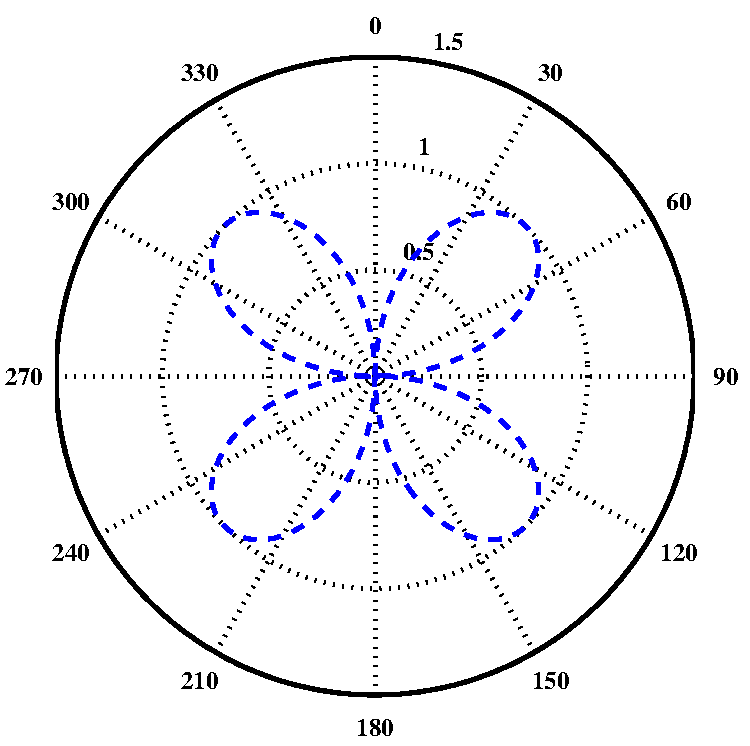
\includegraphics[width=5cm]{Figure/chapter02/radiationpattern/Fig/SP.pdf}}
        \subfloat[]{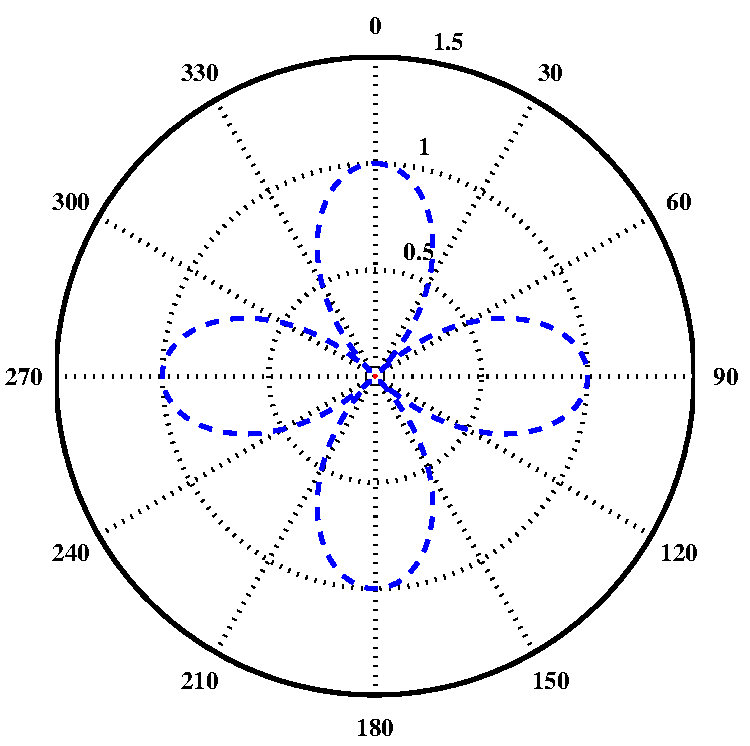
\includegraphics[width=5cm]{Figure/chapter02/radiationpattern/Fig/SS.pdf}}
        \caption{$V_p$(red)和$V_s$
			(blue)扰动的辐射模式。背景波场入射角为$0^{\circ}$,$360^{\circ}$接收不同模式的散射波场。
			 (a) PP, (b) PS, (c) SP和(d) SS模式。
    }
    \label{fig:radiationpattern} 
    \end{center}
\end{figure} 

\subsection{弹性波模式解耦}
弹性波场$\mathbf{u}=(u_x,u_y,u_z)$可以分解成P波波场与S波波场:$\mathbf{u}=\mathbf{u}^P+\mathbf{u}^S$,
其中,$\mathbf{u}^P=(u^P_x,u^P_y,u^P_z)$和$\mathbf{u}^S=(u^S_x,u^S_y,u^S_z)$.
对于各向同性介质而言,模式解耦不依赖于模型参数,可在波数域表示为(Zhang and McMechan, 2010)\cite[]{zhang.mcmechan:2010}:
\begin{equation}
        \tilde{\mathbf U}^P=\mathbf k(\mathbf k\cdot \tilde{\mathbf U}), \quad
        \tilde{\mathbf U}^S=-\mathbf 
        k\times(\mathbf k\times \tilde{\mathbf U})
\label{eq:Decomp}
\end{equation}
其中$\mathbf k=(k_x,k_y,k_z)$ 为归一化之后的波矢量,符号$\tilde{}$表示波数域波场。

根据前文推导, 将Fr{$\acute{e}$}chet导数分解为不同波模式:
\begin{equation}
        {\mathbf J}_M={\mathbf J}^P_M+{\mathbf J}^S_M,
\label{eq:PropaMDall}
\end{equation}
其中
\begin{equation}
        {\mathbf J}^P_M=\mathcal{F}^{-1}(\mathbf k(\mathbf k\cdot \tilde{\mathbf
        J}_M)), \quad
        {\mathbf J}^S_M=\mathcal{F}^{-1}(-\mathbf
                k\times(\mathbf k\times \tilde{\mathbf J}_M)),
\label{eq:PropaMDsplit}
\end{equation}
这里$\mathcal{F}^{-1}$表示从波数域到空间域的反Fourier变换,$\tilde{\mathbf{J}}_M$表示波数域的 Frech{$\acute{e}$}t导数。
这样,方程\eqref{eq:finalMatrixshort}可以按以下方式分裂成两部分:
\begin{equation}
        \mathbf{J}^P\delta\mathbf{m}=\mathbf{\delta u}^P,\quad
        \mathbf{J}^S\delta\mathbf{m}=\mathbf{\delta u}^S,
        \label{eq:UPandUS}
\end{equation}
其中
\begin{equation}
        \mathbf{\delta u}=\mathbf{\delta u}^P+\mathbf{\delta u}^S,
        \label{eq:UPS}
\end{equation}

\begin{equation}
        \mathbf{J}=\mathbf{J}^P+\mathbf{J}^S,
        \label{eq:JPS}
\end{equation}
这里$\mathbf{J}^P=(\mathbf{J}^P_{V_p}\quad\mathbf{J}^P_{V_s})$和$\mathbf{J}^S=(\mathbf{J}^S_{V_p}\quad\mathbf{J}^S_{V_s})$为大小是$K\times{2L}$的矩阵,分别代表P波或S波分量对应的Frech{$\acute{e}$}t导数(Jacobian矩阵)。
方程\eqref{eq:UPandUS}表示了在模式解耦下的Born近似所描述的散射波场。

我们知道,次级震源只有在背景波场入射到参数扰动的位置时才会被激发。尽管次级震源(或者说背景场)中既有P波又有S波,
对于反演来说并不需要严格区分出它们的贡献(原因将在本章讨论部分进行详细阐述)。于是,模式解耦下Jacobian
矩阵满足:
\begin{equation}
        \begin{split} 
        \mathbf{J}^W_M(\mathbf{x}_l,\mathbf{r}_k)=
        \mathbf{T}_M(\mathbf{x}_l):\mathbf{G}'^W(\mathbf{x}_l,\mathbf{r}_k),\quad
        W\in\{P, S\}.
        \end{split}
        \label{eq:EquivFre1}
\end{equation}
该式说明模式解耦算子只作用在$\mathbf{G}'$上,即只作用在散射Green函数的空间导数上。虽然有些学者尝试用“解耦”的方式来
传播P和S波波场(马德堂和朱光明,2003\cite{马德堂2003}; Cheng et al.,
2016\cite{cheng:2016}),
但是只能在介质参数足够光滑的时候才能获得令人满意的结果(Brytik et al., 2011\cite{brytik:2011};
Wang and McMechan, 2015\cite{wang.mcmechan:2015b})。
因此,本文并未采用传播解耦波场的方法,而是用方程\eqref{eq:PropaMDsplit}来对正演后的弹性总波场进行模式解耦。

\section{弹性波模式解耦全波形反演}
方程\eqref{eq:finalMatrixshort}对应的反问题是要找到一个能够解释地震数据的最优模型,它可以通过求解以下
目标函数的最小值问题来实现:
\begin{equation}
    E=\frac{1}{2}\delta\mathbf{d}^{\dagger}\delta\mathbf{d},
    \label{eq:misfit}
\end{equation}
其中$\delta\mathbf{d}$ 表示观测数据与模拟数据之间的残差向量,满足$\delta\mathbf{d}=\mathfrak{F}(\mathbf{u}_{obs}-\mathbf{u}_{cal})$,
这里$\mathfrak{F}$ 为位于接收点处的采样函数,上标$\dagger$表示共轭转置算子。求解该目标函数最小值的标准策略是
采用梯度类或者基于Hessian矩阵的最优化算法。可以通过Jacobian矩阵来求取梯度:
\begin{equation}
        \mathbf{g}=
        \begin{pmatrix}
                \mathbf{g}_{V_p}\\
                \mathbf{g}_{V_s}
        \end{pmatrix}
        =\mathfrak{R}\begin{pmatrix}
                \mathbf{J}^{\dagger}_{V_p}\delta \mathbf{d}\\
                \mathbf{J}^{\dagger}_{V_s}\delta \mathbf{d}
        \end{pmatrix},
        \label{eq:MatrixGra1}
\end{equation}
其中$\mathfrak{R}$表示取实部。为获得模型更新,梯度导引类方法利用下降方向$\mathbf{g}$,而Hessian类方法则利用了
梯度和Hessian矩阵的信息。Hessian类算法能保证二阶的收敛性,但即使是声波FWI也要付出庞大的计算与存储代价。
为了在效率与精度之间寻求平衡,通常会采用梯度类的方法迭代地求解方程\eqref{eq:misfit},即:
\begin{equation}
        \mathbf{m}_{k+1}=\mathbf{m}_{k}-\alpha_k \mathbf{g}_k,
        \label{eq:Gradientmethod1}
\end{equation}
其中$\mathbf{m}$是模型参数向量,$k$是迭代次数,$\alpha_k$和$\mathbf{g}_k$则分别是第$k$次迭代的步长与梯度。
常规的EFWI需要非常多的迭代次数,因此良好的梯度预条件能加速收敛。

方程\eqref{eq:MatrixGra1}中的梯度并没有内在的机制来判断数据残差中的成分是来自$\delta V_p$还是来自$\delta V_s$。
将方程\eqref{eq:MatrixGra1}分裂为P波与S波分量对应的两个部分:
\begin{equation}
        \begin{pmatrix}
                \mathbf{g}^P_{V_p}\\
                \mathbf{g}^P_{V_s}
        \end{pmatrix}
        =\mathfrak{R}\begin{pmatrix}
                [\mathbf{J}^P_{V_p}+\mathbf{J}^S_{V_p}]^{\dagger}\delta \mathbf{d}^P\\
                [\mathbf{J}^P_{V_s}+\mathbf{J}^S_{V_s}]^{\dagger}\delta \mathbf{d}^P
        \end{pmatrix},
        \label{eq:DEMatrixGraP}
\end{equation}
和
\begin{equation}
        \begin{pmatrix}
                \mathbf{g}^S_{V_p}\\
                \mathbf{g}^S_{V_s}
        \end{pmatrix}
        =\mathfrak{R}\begin{pmatrix}
                [\mathbf{J}^P_{V_p}+\mathbf{J}^S_{V_p}]^{\dagger}\delta \mathbf{d}^S\\
                [\mathbf{J}^P_{V_s}+\mathbf{J}^S_{V_s}]^{\dagger}\delta \mathbf{d}^S
        \end{pmatrix},
        \label{eq:DEMatrixGraS}
\end{equation}
其中,$\mathbf{g}^W_M$为特定波模式(W)的数据残差对应的某一物理参数(M)的梯度。
地面多分量地震记录的P/S分离非常具有挑战,因此数据残差的分解也会变得非常困难,尤其是在近地表介质不均匀且(或者)
边界条件不完整的情况下。因此尽量采取策略来回避多分量地震记录的地面P/S分离。
\begin{figure}
    \begin{center}
        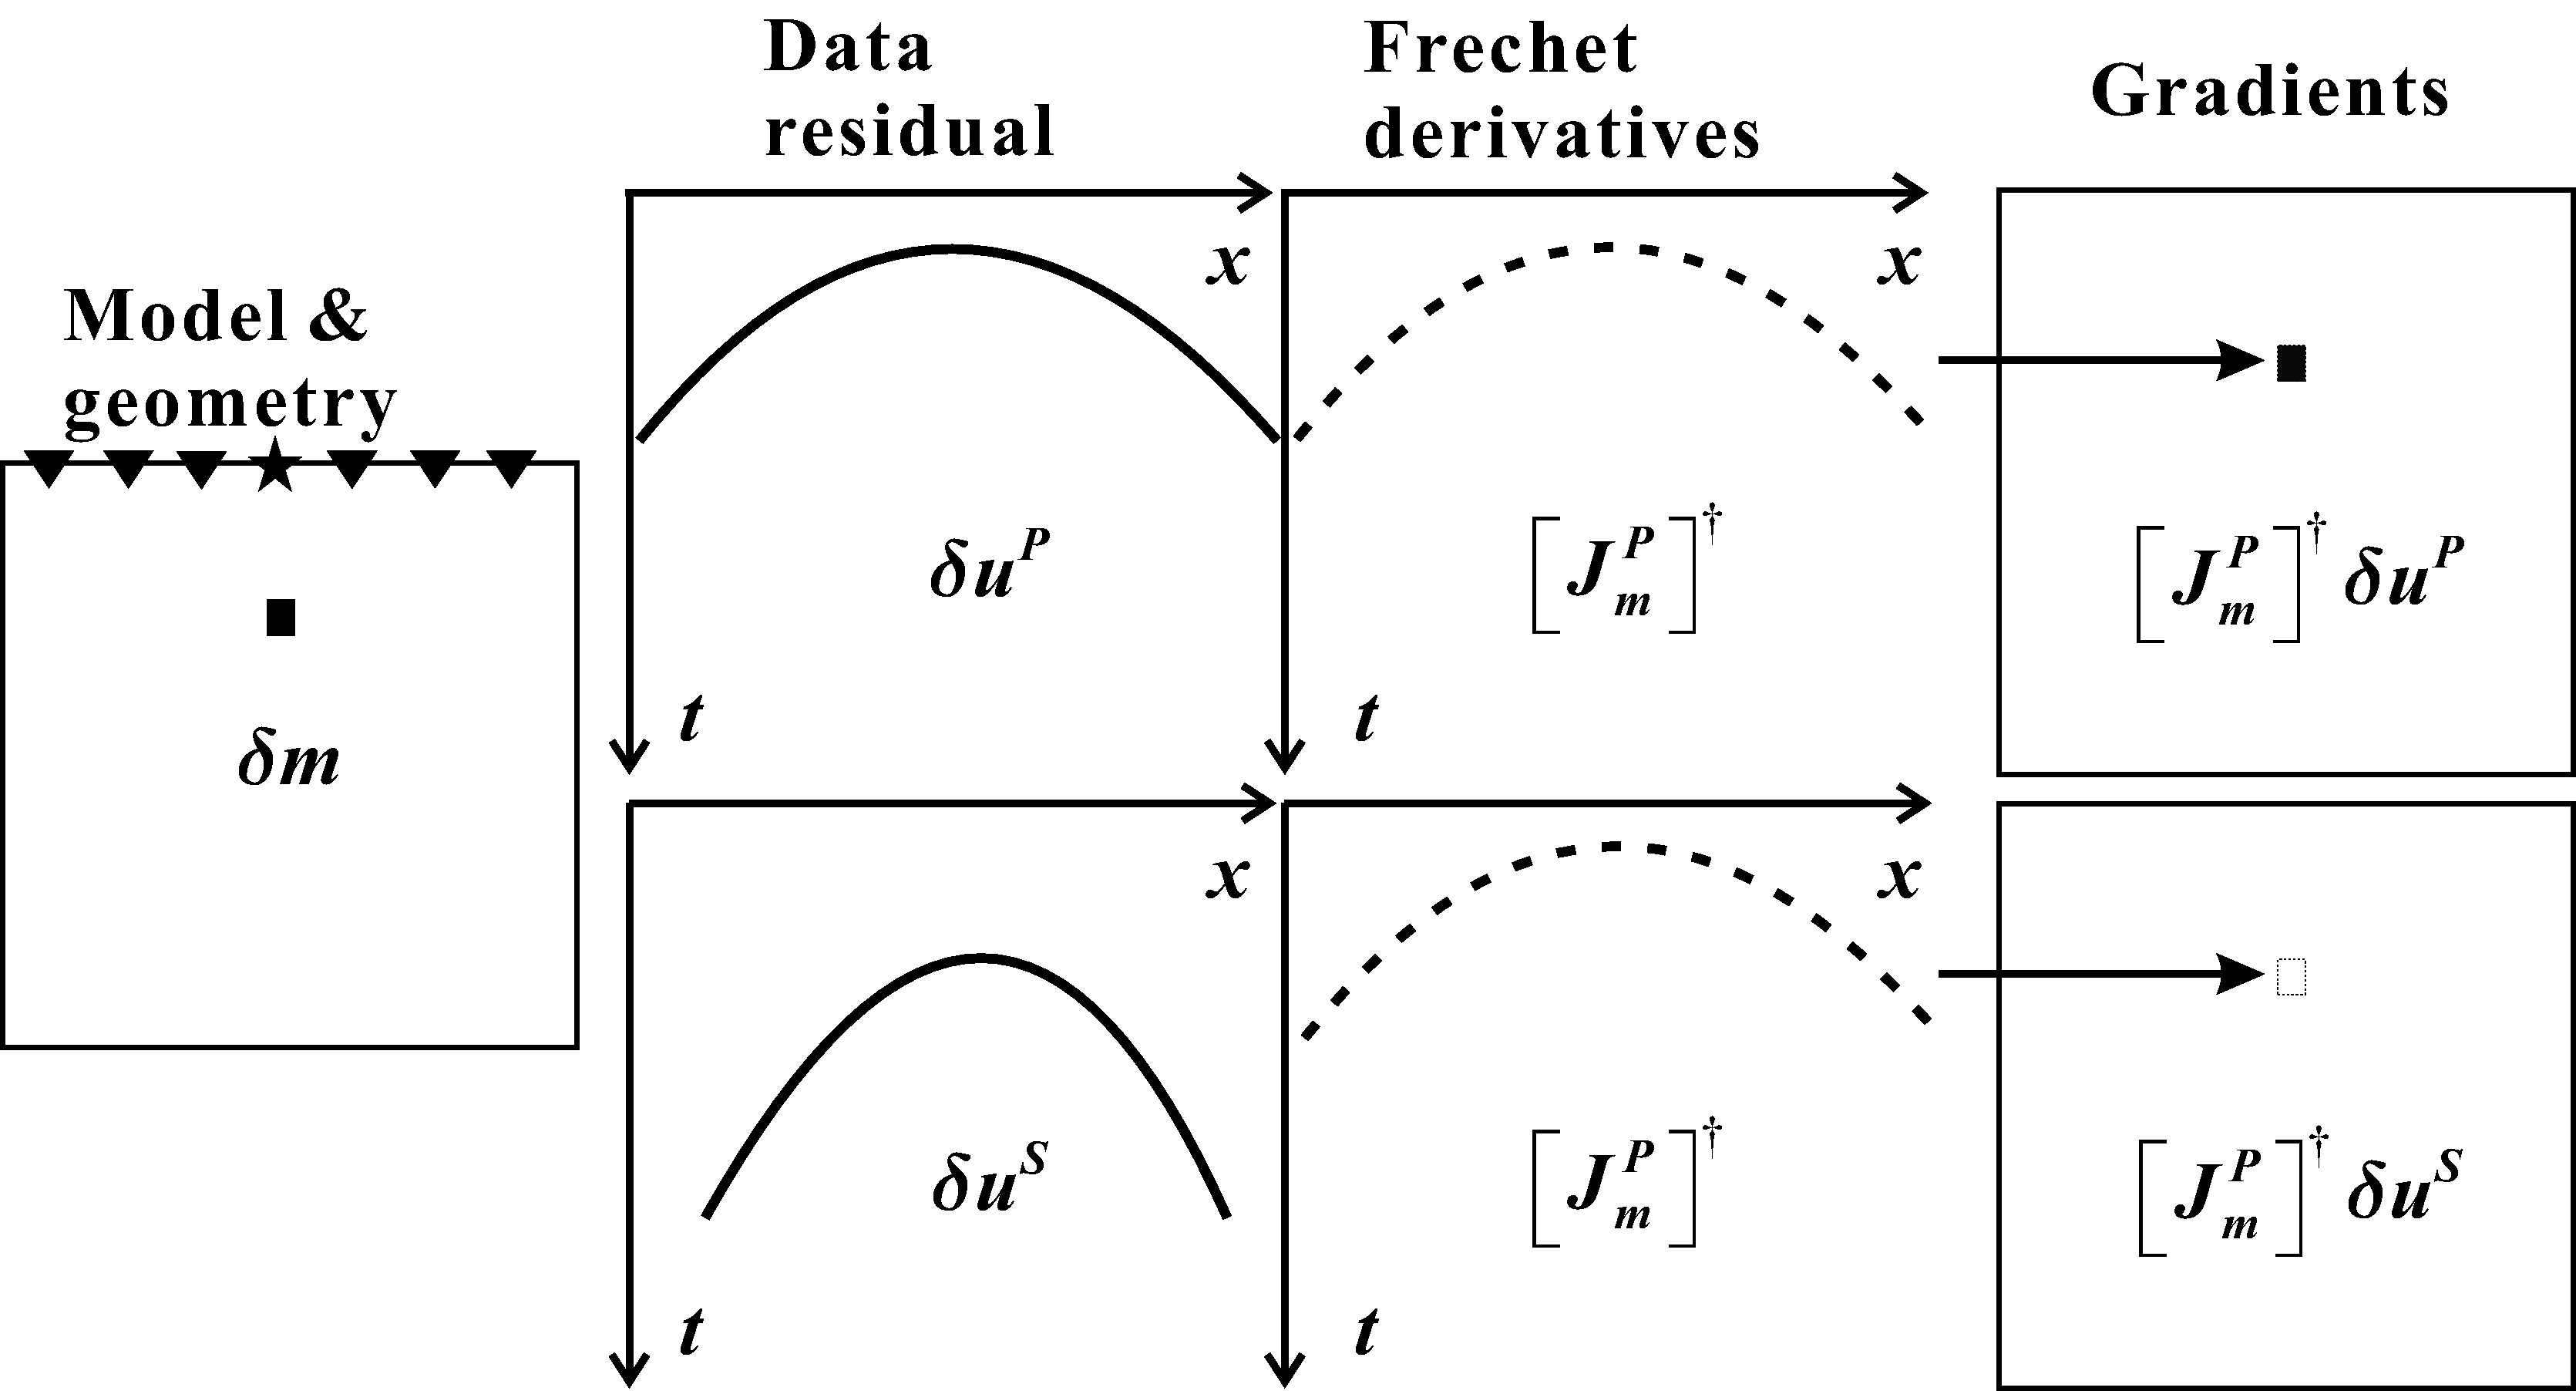
\includegraphics[width=1.0\textwidth]{Figure/chapter02/finalMarmousiII/Fig/zerolagLAST1.pdf}
        \caption{
			通过偏导数波场与数据残差之间的零延迟互相关计算梯度的示意图。为了简单说明,只在背景介质中放置一个的散射点。
%Schematic illustration of gradient calculation through zero-lag correlation
% between the partial derivative wavefields
%and the residual seismogram.
%Only a point perturbation is given in the background media for illustration.
    }
    \label{fig:crossterm}
    \end{center}
\end{figure}

目标函数的梯度可看作是偏导数波场与数据残差在时间域的零延迟互相关\cite[]{pratt1998gauss}。如图\ref{fig:crossterm}所示,
假设背景介质中有一个点扰动,数据残差为观测数据与模拟数据之间的差值。偏导数波场代表了由次级源产生的特征性点绕射响应。
一般而言,P波与S波背景速度不同,因而在偏导数波场和地震记录残差中它们的运动学特征(比如走时和曲率)也不同。
所以,相同波模式之间的零延迟互相关将在梯度计算中占主导地位,而不同波模式之间的互相关则会由于非同相的干涉叠加被基本消除掉。
因此,会有以下的交叉项近似:
\begin{equation}
        \begin{split}
                [\mathbf{J}_{V_p}^{S}]^{\dagger}\delta \mathbf{d}^P\approx\mathbf{0},\\
                [\mathbf{J}_{V_s}^{S}]^{\dagger}\delta \mathbf{d}^P\approx\mathbf{0},\\
                [\mathbf{J}_{V_p}^{P}]^{\dagger}\delta \mathbf{d}^S\approx\mathbf{0},\\
                [\mathbf{J}_{V_s}^{P}]^{\dagger}\delta \mathbf{d}^S\approx\mathbf{0},
        \end{split}
        \label{eq:crossterms}
\end{equation}
其中$\mathbf{0}$为空矩阵。
此外,散射模式说明P波速度的扰动不会产生S波散射,所以还有:
\begin{equation}
\mathbf{J}^S_{V_p}=\mathbf{0}.
\label{eq:Jsvp}
\end{equation}
从而得到:
\begin{equation}
        \begin{split}
[\mathbf{J}^S_{V_p}]^{\dagger}\delta \mathbf{d}^P=\mathbf{0}, \\
[\mathbf{J}^S_{V_p}]^{\dagger}\delta \mathbf{d}^S=\mathbf{0}.
        \end{split}
\label{eq:Jsvp1}
\end{equation}
\subsection{模式解耦梯度预条件}
利用方程\eqref{eq:crossterms}和\eqref{eq:Jsvp1},可以获得以下近似:
\begin{equation}
        \mathbf{J}^{\dagger}_{V_p}\delta \mathbf{d}^P\approx
        [\mathbf{J}^P_{V_p}]^{\dagger}\delta \mathbf{d},\quad
        \mathbf{J}^{\dagger}_{V_s}\delta \mathbf{d}^S\approx
        [\mathbf{J}^S_{V_s}]^{\dagger}\delta \mathbf{d}.
        \label{eq:crossterm}
\end{equation}
因此,基于模式解耦的梯度可以表示为:
\begin{equation}
        \begin{pmatrix}
                \mathbf{g}^P_{V_p}\\
                \mathbf{g}^P_{V_s}
        \end{pmatrix}
        \approx\mathfrak{R}\begin{pmatrix}
                [\mathbf{J}_{V_p}^{P}]^{\dagger}\delta \mathbf{d}\\
                [\mathbf{J}_{V_s}^{P}]^{\dagger}\delta \mathbf{d}
        \end{pmatrix},
        \label{eq:MatrixGraP}
\end{equation}
和
\begin{equation}
        \begin{pmatrix}
                \mathbf{g}^S_{V_p}\\ 
                \mathbf{g}^S_{V_s}
        \end{pmatrix}
        \approx\mathfrak{R}\begin{pmatrix}
                \mathbf{0}\\ 
                [\mathbf{J}^S_{V_s}]^{\dagger}\delta \mathbf{d}
        \end{pmatrix}.
        \label{eq:MatrixGraS}
\end{equation}
上述方程表明在梯度计算中可以通过Fr{$\acute{e}$}chet导数的解耦来代替数据残差的解耦。

进一步而言,由于串扰效应主要体现在P波数据中,因此本文提出舍弃梯度中的$\mathbf{g}_{V_s}^P$项来降低参数耦合效应。
于是,分别选取解耦后的P波与S波Fr{$\acute{e}$}chet导数来构建预条件之后$V_p$和$V_s$的梯度:
\begin{equation}
        \begin{pmatrix}
                \hat{\mathbf{g}}_{V_p}\\
                \hat{\mathbf{g}}_{V_s}
        \end{pmatrix}=
        \begin{pmatrix}
                \mathbf{g}_{V_p}^P\\
                \mathbf{g}_{V_s}^S
        \end{pmatrix}
        \approx 
        \mathfrak{R}\begin{pmatrix}
                [\mathbf{J}^P_{V_p}]^{\dagger} \delta \mathbf{d}\\
                [\mathbf{J}^S_{V_s}]^{\dagger} \delta \mathbf{d}
        \end{pmatrix}.
        \label{eq:MatrixGraMode}
\end{equation}
这里符号$\hat{}$指示基于模式解耦的预条件梯度。
最终,EFWI问题转化为通过模式解耦预条件共轭梯度(MDPCG)的方式来迭代求解:
\begin{equation}
        \mathbf{m}_{k+1}=\mathbf{m}_{k}-\alpha_k
        \begin{bmatrix}\mathbf{Q}_1\hat{\mathbf{g}}_{V_p}\\\mathbf{Q}_2\hat{\mathbf{g}}_{V_s}\end{bmatrix}_{k},
        \label{eq:Gradientmethod}
\end{equation}
其中,$\mathbf{Q}_1$和$\mathbf{Q}_2$表示进一步的预条件算子,比如采用能量照明对梯度进行补偿。步长$\alpha_k$采用抛物线拟合的方式来搜寻(Vigh
and Starr, 2008\cite[]{vigh20083d})。

\subsection{伴随状态法计算梯度}
显式地计算Fr{$\acute{e}$}chet导数需要进行多达模型网格数量的正演模拟次数,这在目前实际应用中无法实现\cite[]{virieux2009overview}。
为了避免显式构建Jacobian矩阵,文中采用伴随状态法来计算梯度\cite[]{tromp2005seismic,plessix2006}。利用Green函数的空间互易性,
方程\eqref{eq:MatrixGra1}中的原始梯度可以通过正传波场与反传的残差波场的时间域
零延迟互相关计算得到:
\begin{equation} 
        \begin{split}
        \mathbf{g}_{V_p}&=-2\rho V_p\int_{0}^{T}\frac{\partial u_i}{\partial
        x_j}\frac{\partial \psi_k}{\partial x_l}
        \delta_{ij}\delta_{kl}dt,\\
        \mathbf{g}_{V_s}&=-2\rho V_s\int_{0}^{T}\frac{\partial u_i}{\partial
        x_j}\frac{\partial \psi_k}{\partial x_l}
        (-2\delta_{ij}\delta_{kl}+\delta_{ik}\delta_{jl}+\delta_{il}\delta_{jk})dt,
        \end{split}
        \label{eq:Gradient_vpvs}
\end{equation}
其中$u_i$是从震源出发的正传波场,$\psi_k$ 为由数据残差从接收点处反传重建的伴随波场。注意方程\eqref{eq:Gradient_vpvs}
中第一行的算式中自动隐含了正传和伴随波场的散度算子。

从方程\eqref{eq:EquivFre1}可看出,Frech$\acute{e}$t导数的模式解耦等价于施加在散射Green函数上。这就意味着当使用伴随状态法时,
只需要解耦伴随波场就可以获得预条件后的梯度,即:
\begin{equation} 
        \begin{split} 
                \hat{\mathbf{g}}_{V_p}&=-2\rho V_p\int_{0}^{T}\frac{\partial u_i}{\partial
        x_j}\frac{\partial \psi^P_k}{\partial x_l}
        \delta_{ij}\delta_{kl}dt,\\
        &=-2\rho V_p\int_{0}^{T}\frac{\partial u_i}{\partial
        x_j}\frac{\partial \psi_k}{\partial x_l}
        \delta_{ij}\delta_{kl}dt,\\
                \hat{\mathbf{g}}_{V_s}&=-2\rho V_s\int_{0}^{T}\frac{\partial u_i}{\partial
        x_j}\frac{\partial \psi^S_k}{\partial x_l}
        (\delta_{ik}\delta_{jl}+\delta_{il}\delta_{jk})dt,
        \end{split}
        \label{eq:DeGradient_vpvs} 
\end{equation}
其中$\psi^P$和$\psi^S$分别为P波和S波的伴随波场。由于$\mathbf{g}_{V_p}$的计算中隐含了散度算子,总是满足$\hat{\mathbf{g}}_{V_p}=\mathbf{g}_{V_p}$。
与方程\eqref{eq:Gradient_vpvs}对比,由于S波的散度总是为0,所以在计算预条件后的$V_s$梯度时舍弃了$-2\delta_{ij}\delta_{kl}$项。
因此,对于P波速度而言,模式解耦已经自动隐含在梯度计算中,但是对$V_s$梯度的模式解耦预条件需要显式地施加。

解耦伴随波场需要额外的计算量,主要体现在每个时间片中需要两次Fourier变换。为了减少计算量并节省内存消耗,可以
对正传波场与反传波场在时间轴上进行重采样,并且在互相关之前只对反传的伴随波场进行模式解耦。
当考虑其它多尺度策略考虑时,也可以对正传波场进行解耦,例如在某一阶段反演中单独使用SS或者PS波模式的数据。但本文并不推荐
这样的策略,这将在讨论部分进行阐述。
\section{模式解耦降低参数耦合的理论机制}
	前一节提出了通过模式解耦来预条件处理EFWI的梯度,以便压制参数耦合效应。然而解决参数解耦问题最直接有效(但也最昂贵)
的方法是考虑Hessian矩阵的优化方法。下面将采用解耦后的
Frech$\acute{e}$t导数来调查Hessian和分辨率矩阵的性质,并且对比常规(PCG)、模式解耦(MDPCG)和高斯-牛顿(GN)的梯度来
阐明模式解耦EFWI压制参数耦合的内在机制。
\subsection{Hessian矩阵及其不同模式的分量}
多参数情况下的Hessian矩阵是一个具有块状结构的对称方阵,其中非对角块测量了不同物理参数的偏导数波场之间的互相关效应,其作用
是消除多参数反演中的参数耦合效应。当反问题为近似线性或者数据残差非常小的时候,全Hessian将约等于近似Hessian
\cite[]{pratt1998gauss}:
\begin{equation}
\mathbf{H}_a =\mathfrak{R}[{\mathbf{J}}^{\dagger}\mathbf{J}]. 
\label{eq:hess}
\end{equation}
考虑到Fr{$\acute{e}$}chet导数的解耦(见方程\ref{eq:JPS}),可以将 $\mathbf{H}_a$ 分解为四个分量:
\begin{equation}
\begin{split}
\mathbf{H}_a^{PP}=\mathfrak{R}[{\mathbf{J}^{P}}]^{\dagger}[{\mathbf{J}^{P}}],\\
\mathbf{H}_a^{PS}=\mathfrak{R}[{\mathbf{J}^{P}}]^{\dagger}[{\mathbf{J}^{S}}],\\
\mathbf{H}_a^{SP}=\mathfrak{R}[{\mathbf{J}^{S}}]^{\dagger}[{\mathbf{J}^{P}}],\\
\mathbf{H}_a^{SS}=\mathfrak{R}[{\mathbf{J}^{S}}]^{\dagger}[{\mathbf{J}^{S}}].
\end{split}
\label{eq:hessian_component}
\end{equation}

\begin{figure}[!htb]
    \begin{center}
        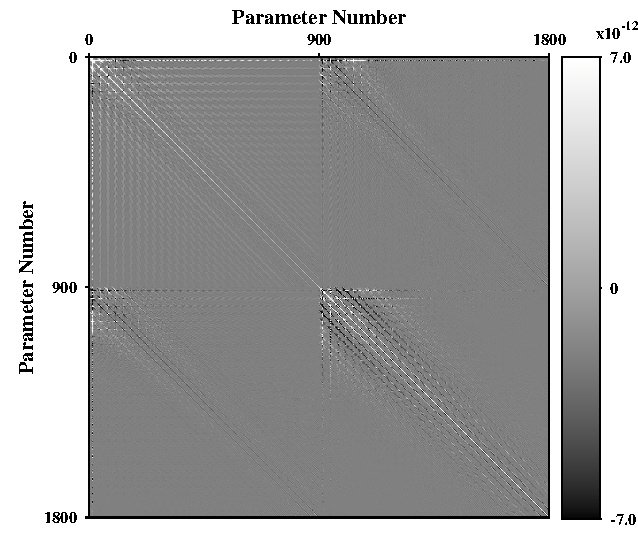
\includegraphics[width=10cm]{Figure/chapter02/ResoOpera/Fig/hessian.pdf}
        \caption{
            近似Hessian矩阵$\mathbf{H}_a$.
    }
    \label{fig:Hessian} 
    \end{center}
\end{figure}
\begin{figure}[!htb]
    \begin{center}
        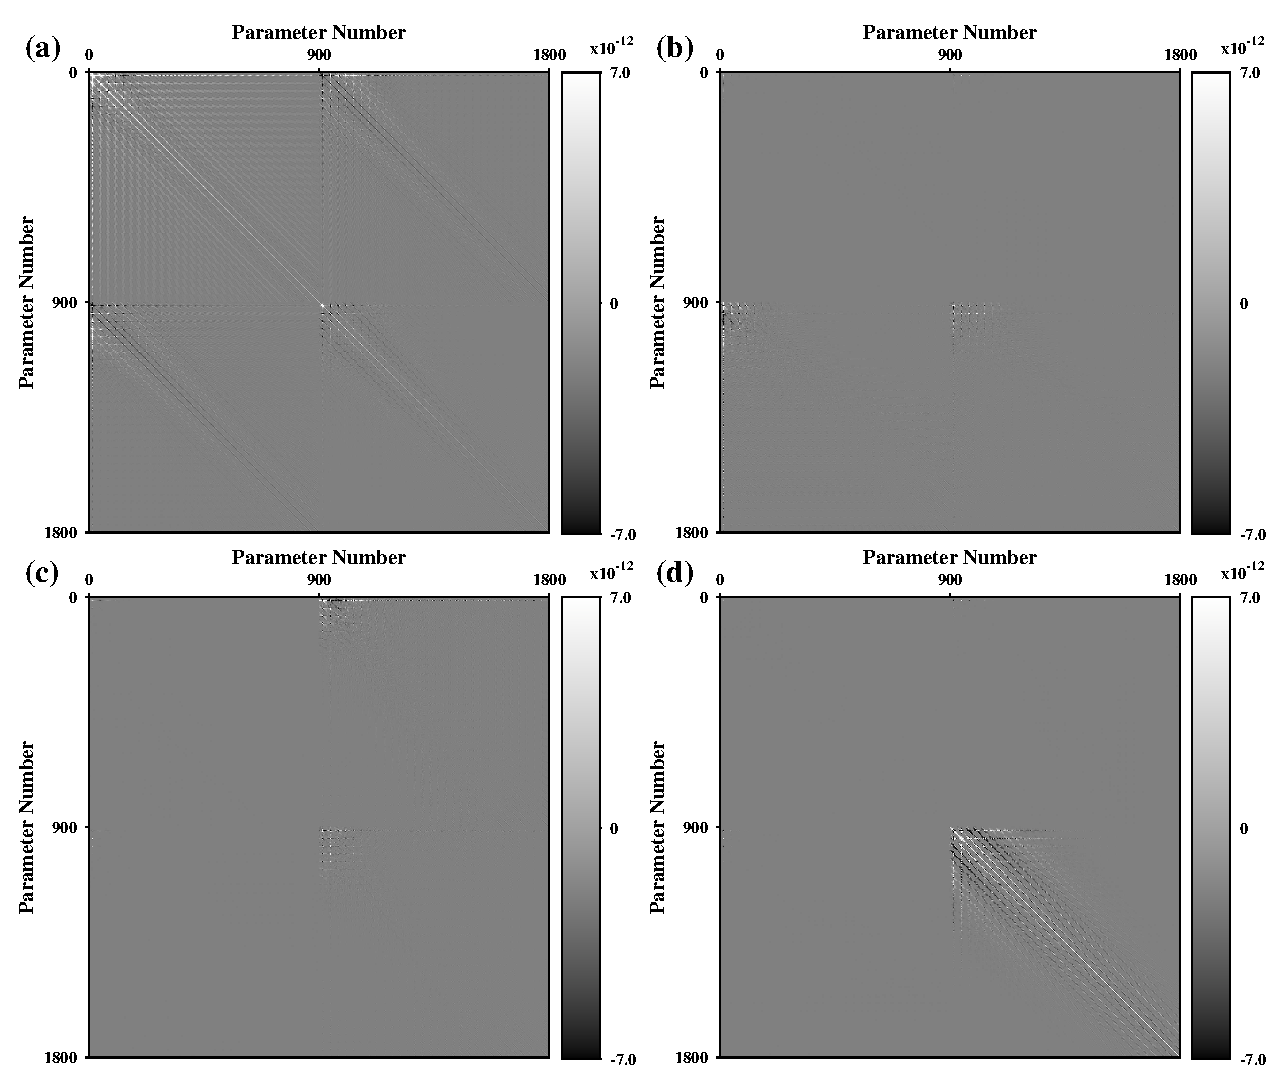
\includegraphics[width=12cm]{Figure/chapter02/ResoOpera/Fig/fourhessian.pdf}
        \caption{
            近似Hessian矩阵的四个分量:
                        (a) $\mathbf{H}_a^{PP}$,
            (b) $\mathbf{H}_a^{PS}$, (c) $\mathbf{H}_a^{SP}$ and (d)$\mathbf{H}_a^{SS}$.
    }
    \label{fig:fourHessian}
    \end{center}
\end{figure}
从大规模应用问题来讲,Hessian矩阵通常是无法计算的。为了调查每个分量各自的贡献,这里在一个网格大小为$30\times30$,
空间采样为5m的模型上数值地计算出Hessian矩阵的各个分量。在模型的顶部中央放置一个纯P波震源,接收点分布于四个边界上。
近似Hessian矩阵(图\ref{fig:Hessian})及其分量(图\ref{fig:fourHessian})通过时间域的
Frech{$\acute{e}$}t导数显式
计算,$H_a$中非对角块中明显的非零元素代表了很强的参数耦合效应。可以观察到以下
现象:
首先,交叉项分量($\mathbf{H}_a^{PS}$和$\mathbf{H}_a^{SP}$)对$\mathbf{H}_a$的贡献可以忽略不计。这是由于
背景P波和S波速度不同导致
相应
的P波与S波Fr{$\acute{e}$}chet导数
不具有相干性。
注意到,在这些交叉项分量中会有一些非常小值的非零元素。
这是由于Fr{$\acute{e}$}chet导数中震源附近的异常值所导致的。故有:
\begin{equation}
        \mathbf{H}_a\approx
        \mathbf{H}_a^{PP}+
        \mathbf{H}_a^{SS}.
        \label{eq:C3}
\end{equation}
其次,$\mathbf{H}_a$的非对角区块几乎与$\mathbf{H}_a^{PP}$一样,并且$\mathbf{H}_a^{SS}$只在右下对角快是非零的,
这是因为$\mathbf{J}^S=(\mathbf{0}\quad\mathbf{J}^S_{V_s})$。这些现象进一步确认了参数耦合主要是来自P波波场而非S波波场。
\subsection{模型分辨率矩阵及其分量}
通过模式解耦的Frech{$\acute{e}$}t导数对Hessian矩阵的定性分析并不足以理解模式解耦对反演产生作用的机制。为了评估P波与S波数据对
反演的贡献,我们进一步分析模式解耦如何在模型空间影响分辨率矩阵。模型的分辨率矩阵通常采用Hessian矩阵及其逆矩阵来计算得到
(Menke, 1989\cite[]{menke:1989}; Snieder and Trampert, 1999\cite{snieder1999inverse})。就方程\eqref{eq:finalMatrixshort}对应的反问题,采用以下公式来更新模型:
\begin{equation}
	\delta \tilde{\mathbf{m}}=-\mathbf{H}^{-1}_a\mathbf{J}^{\dagger}\delta 
        \mathbf{d},
        \label{eq:LeastSol}
\end{equation}
其中$\delta\tilde{\mathbf{m}}$为用全部数据残差估计得到的模型扰动。根据Born近似$\delta\mathbf{d}=\mathfrak{F}{\delta\mathbf{u}}$,
将方程\eqref{eq:finalMatrixshort}带入到式\eqref{eq:LeastSol}中,并省略采样函数$\mathfrak{F}$,可得:
\begin{equation}
	\delta \tilde{\mathbf{m}}=\mathbf{R}\delta \mathbf{m},
	\label{eq:ResoMatr}
\end{equation}
其中$\delta \mathbf{m}$表示真实模型扰动,且模型分辨率矩阵$\mathbf{R}$满足:
\begin{equation}
        \mathbf{R}=-\mathbf{H}^{-g}_a\mathbf{H}_a. 
        \label{eq:ResoOper} 
\end{equation}
注意,由于有限的观测导致近似Hessian总是病态的,因此这里采用Hessian的伪逆(广义逆)$\mathbf{H}^{-g}_a$,而不是真实的逆$\mathbf{H}^{-1}_a$。

\begin{figure*}
    \begin{center}
        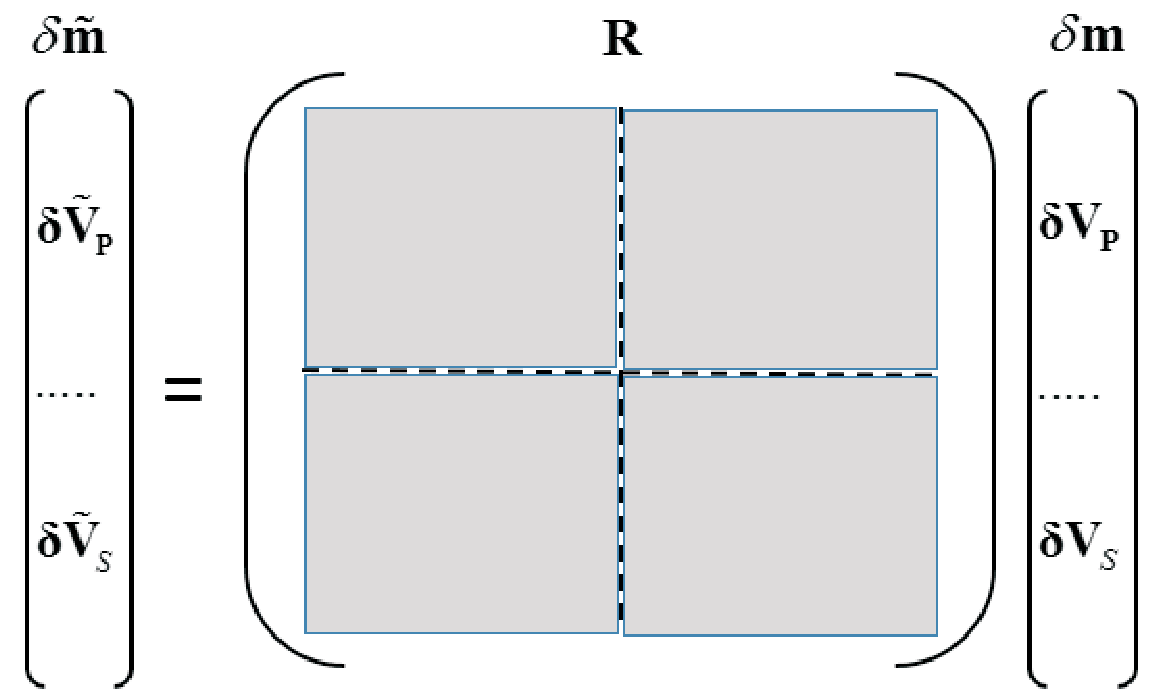
\includegraphics[width=10cm]{Figure/chapter02/ResoOpera/Fig/resolutionmatrix.pdf}
        \caption{
			分辨率矩阵示意图。对于双参数的反问题,分辨率矩阵可以分成四个区块。
    }
    \label{fig:IllustrReso}
    \end{center}
\end{figure*}
如图\ref{fig:IllustrReso}所示,模型分辨率矩阵可看作是作用在真实模型上的滤波器。如果观测手段足够好,则分辨率矩阵会是严格的单位矩阵,
即$\mathbf{R}=\mathbf{I}$,那么模型参数也会是唯一确定的。然而,通常情况下$\mathbf{R} \ne \mathbf{I}$,因此对模型的估计将是真实模型参数的加权平均值。
$\mathbf{R}$ 的对角区块隐含了单参数内部间的相互影响及其相应的分辨能力,而非对角区块则反映了不同参数之间的相互影响。如果对角区块上有明显的非零元素分布,
则预示着不可忽视的参数耦合效应。若采用分解后的P波数据,则方程\eqref{eq:LeastSol} 变为:
\begin{equation}
        \delta \tilde{\mathbf{m}}^P=-\mathbf{H}^{-1}_a\mathbf{J}^{\dagger}\delta \mathbf{d}^P,
        \label{eq:LeastSolP}
\end{equation}
其中$\delta \tilde{\mathbf{m}}^P$ 表示P波数据给出的模型估计。同样采用式\eqref{eq:LeastSol}至式\eqref{eq:ResoOper}的推导,
可得P波数据的模型分辨率矩阵:
\begin{equation}
        \mathbf{R}^P=-\mathbf{H}^{-g}_a\mathbf{H}_a^P,
        \label{eq:ResoOperP}
\end{equation}
其中$\mathbf{H}_a^P=\mathbf{J}^{\dagger}\mathbf{J}^P$。类似的,S波的分辨率矩阵为:
\begin{equation}
        \mathbf{R}^S=-\mathbf{H}^{-g}_a\mathbf{H}_a^S,
        \label{eq:ResoOperS}
\end{equation}
且$\mathbf{H}_a^S=\mathbf{J}^{\dagger}\mathbf{J}^S$。容易证明$\mathbf{R}=\mathbf{R}^P+\mathbf{R}^S$。

\begin{figure}[!bht]
    \begin{center}
        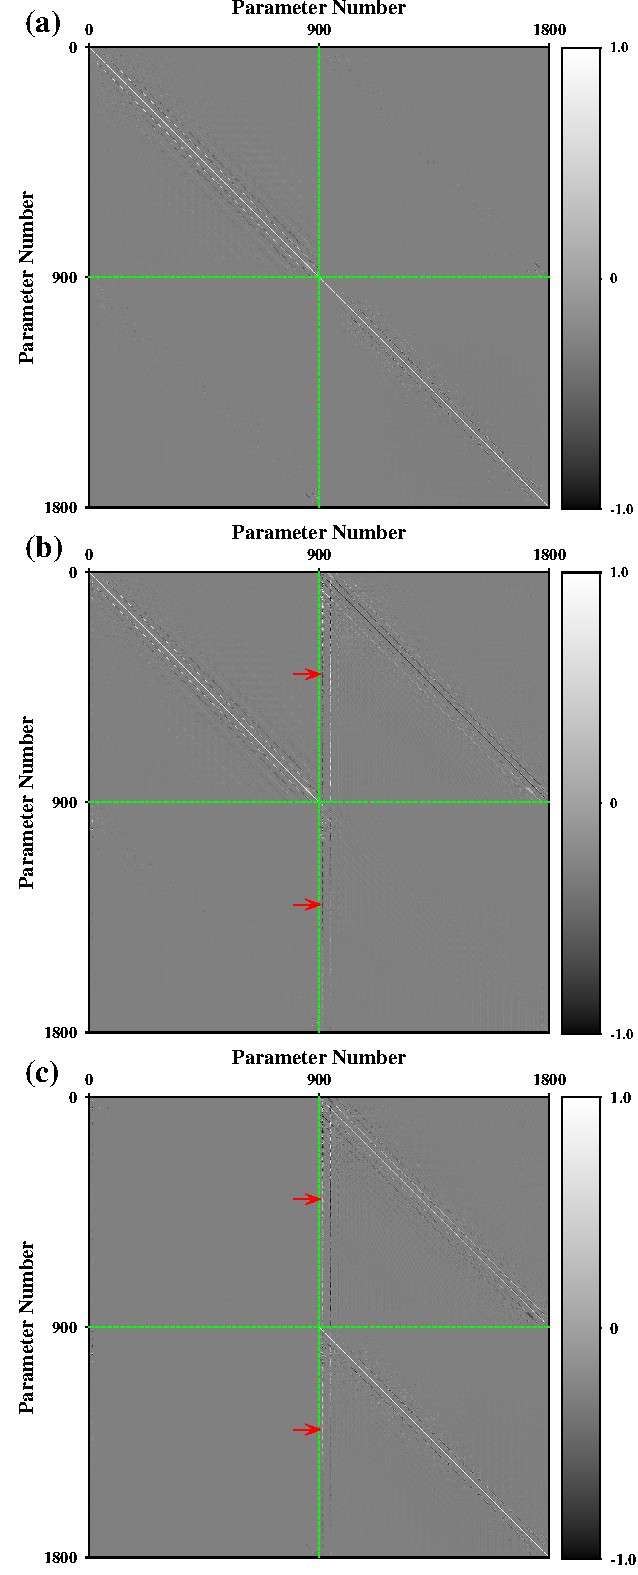
\includegraphics[width=8cm]{Figure/chapter02/ResoOpera/Fig/resolutionoriginal.pdf}
        \caption{
分辨率矩阵及其不同波模式的分量
%Resolution matrix and its components:
(a) $\mathbf{R}$, (b) $\mathbf{R}^P$ and (c) $\mathbf{R}^S$.
    }
    \label{fig:Resolution}
    \end{center}
\end{figure}
同样采用前文小模型,可以显式计算出模型分辨率矩阵$\mathbf{R}$,$\mathbf{R}^P$和$\mathbf{R}^S$。
原始分辨率矩阵(图\ref{fig:Resolution}a)为带状对角阵,对角元素为小于1的正值。这说明了近似Hessian的逆可以为$V_p$和$V_s$的反演
提供很好的预条件。P波与S波数据对应的分辨率矩阵(图\ref{fig:Resolution}b和c)展示了一些有趣的现象。例如,$\mathbf{R}^P$和$\mathbf{R}^S$的对角块
构成了$\mathbf{R}$。除了一些由于震源附近的干扰而导致的假象,$\mathbf{R}^P$的底部两个区块都为空矩阵。在$\mathbf{R}^P$和$\mathbf{R}^S$的右上区块,它们的元素值
大小相等符号相反,两者相加为零从而能够使得$\mathbf{R}$右上区块为空。这些特征说明,对于线性的反问题(无cycle-skipping),P波与S波都对反演$V_p$有贡献,
而P波对$V_s$的贡献非常弱。常规的梯度法由于只用P波数据来计算$V_p$梯度(见式\ref{eq:Gradient_vpvs}),而这部分P波数据有可能来自$V_s$扰动,从而导致反演受到
参数耦合的影响。此外,单独用S波数据可以很好的分辨$V_s$。模式解耦的预条件方式正好利用了上述特征,因而其能够压制反演中参数间的耦合。
\subsection{与Gauss-Newton梯度的比较}
GN方法利用近似Hessian的逆对梯度进行预条件来处理参数之间的耦合效应:
\begin{equation}
\delta\tilde{\mathbf{m}} = - \mathbf{H}^{-1}_a\mathbf{g}.
\label{eq:GN}
\end{equation}
假设$\mathbf{H}_a$的伪逆为:
\begin{equation}
        \mathbf{H}^{-g}_a=    
        \begin{bmatrix}
                \mathbf{D}&\mathbf{E} \\
                \mathbf{F}&\mathbf{G}
        \end{bmatrix},
        \label{eq:HessInv}
\end{equation}
则GN方法实际上利用以下公式来更新模型:
\begin{equation}
    \mathbf{{m}}_{k+1}
    =\mathbf{{m}}_{k}-\alpha_k 
    \begin{bmatrix}
        \mathbf{D}\mathbf{g}^P_{V_p} +
        \mathbf{E}\mathbf{g}^P_{V_s}+
        \mathbf{E}\mathbf{g}^S_{V_s}\\
        \mathbf{G}\mathbf{g}^S_{V_s}
    \end{bmatrix}_{k},
    \label{eq:PreGNFi}
\end{equation}
因为
\begin{equation}
        \delta \mathbf{V}^P_s\approx0, \quad \delta \mathbf{V}_s \approx \delta
        \mathbf{V}^S_s=-\mathbf{G}\mathbf{g}^S_{V_s},
        \label{eq:KeyPoint}
\end{equation}
(见附录A)。
\begin{figure}[!thb]
    \begin{center}
        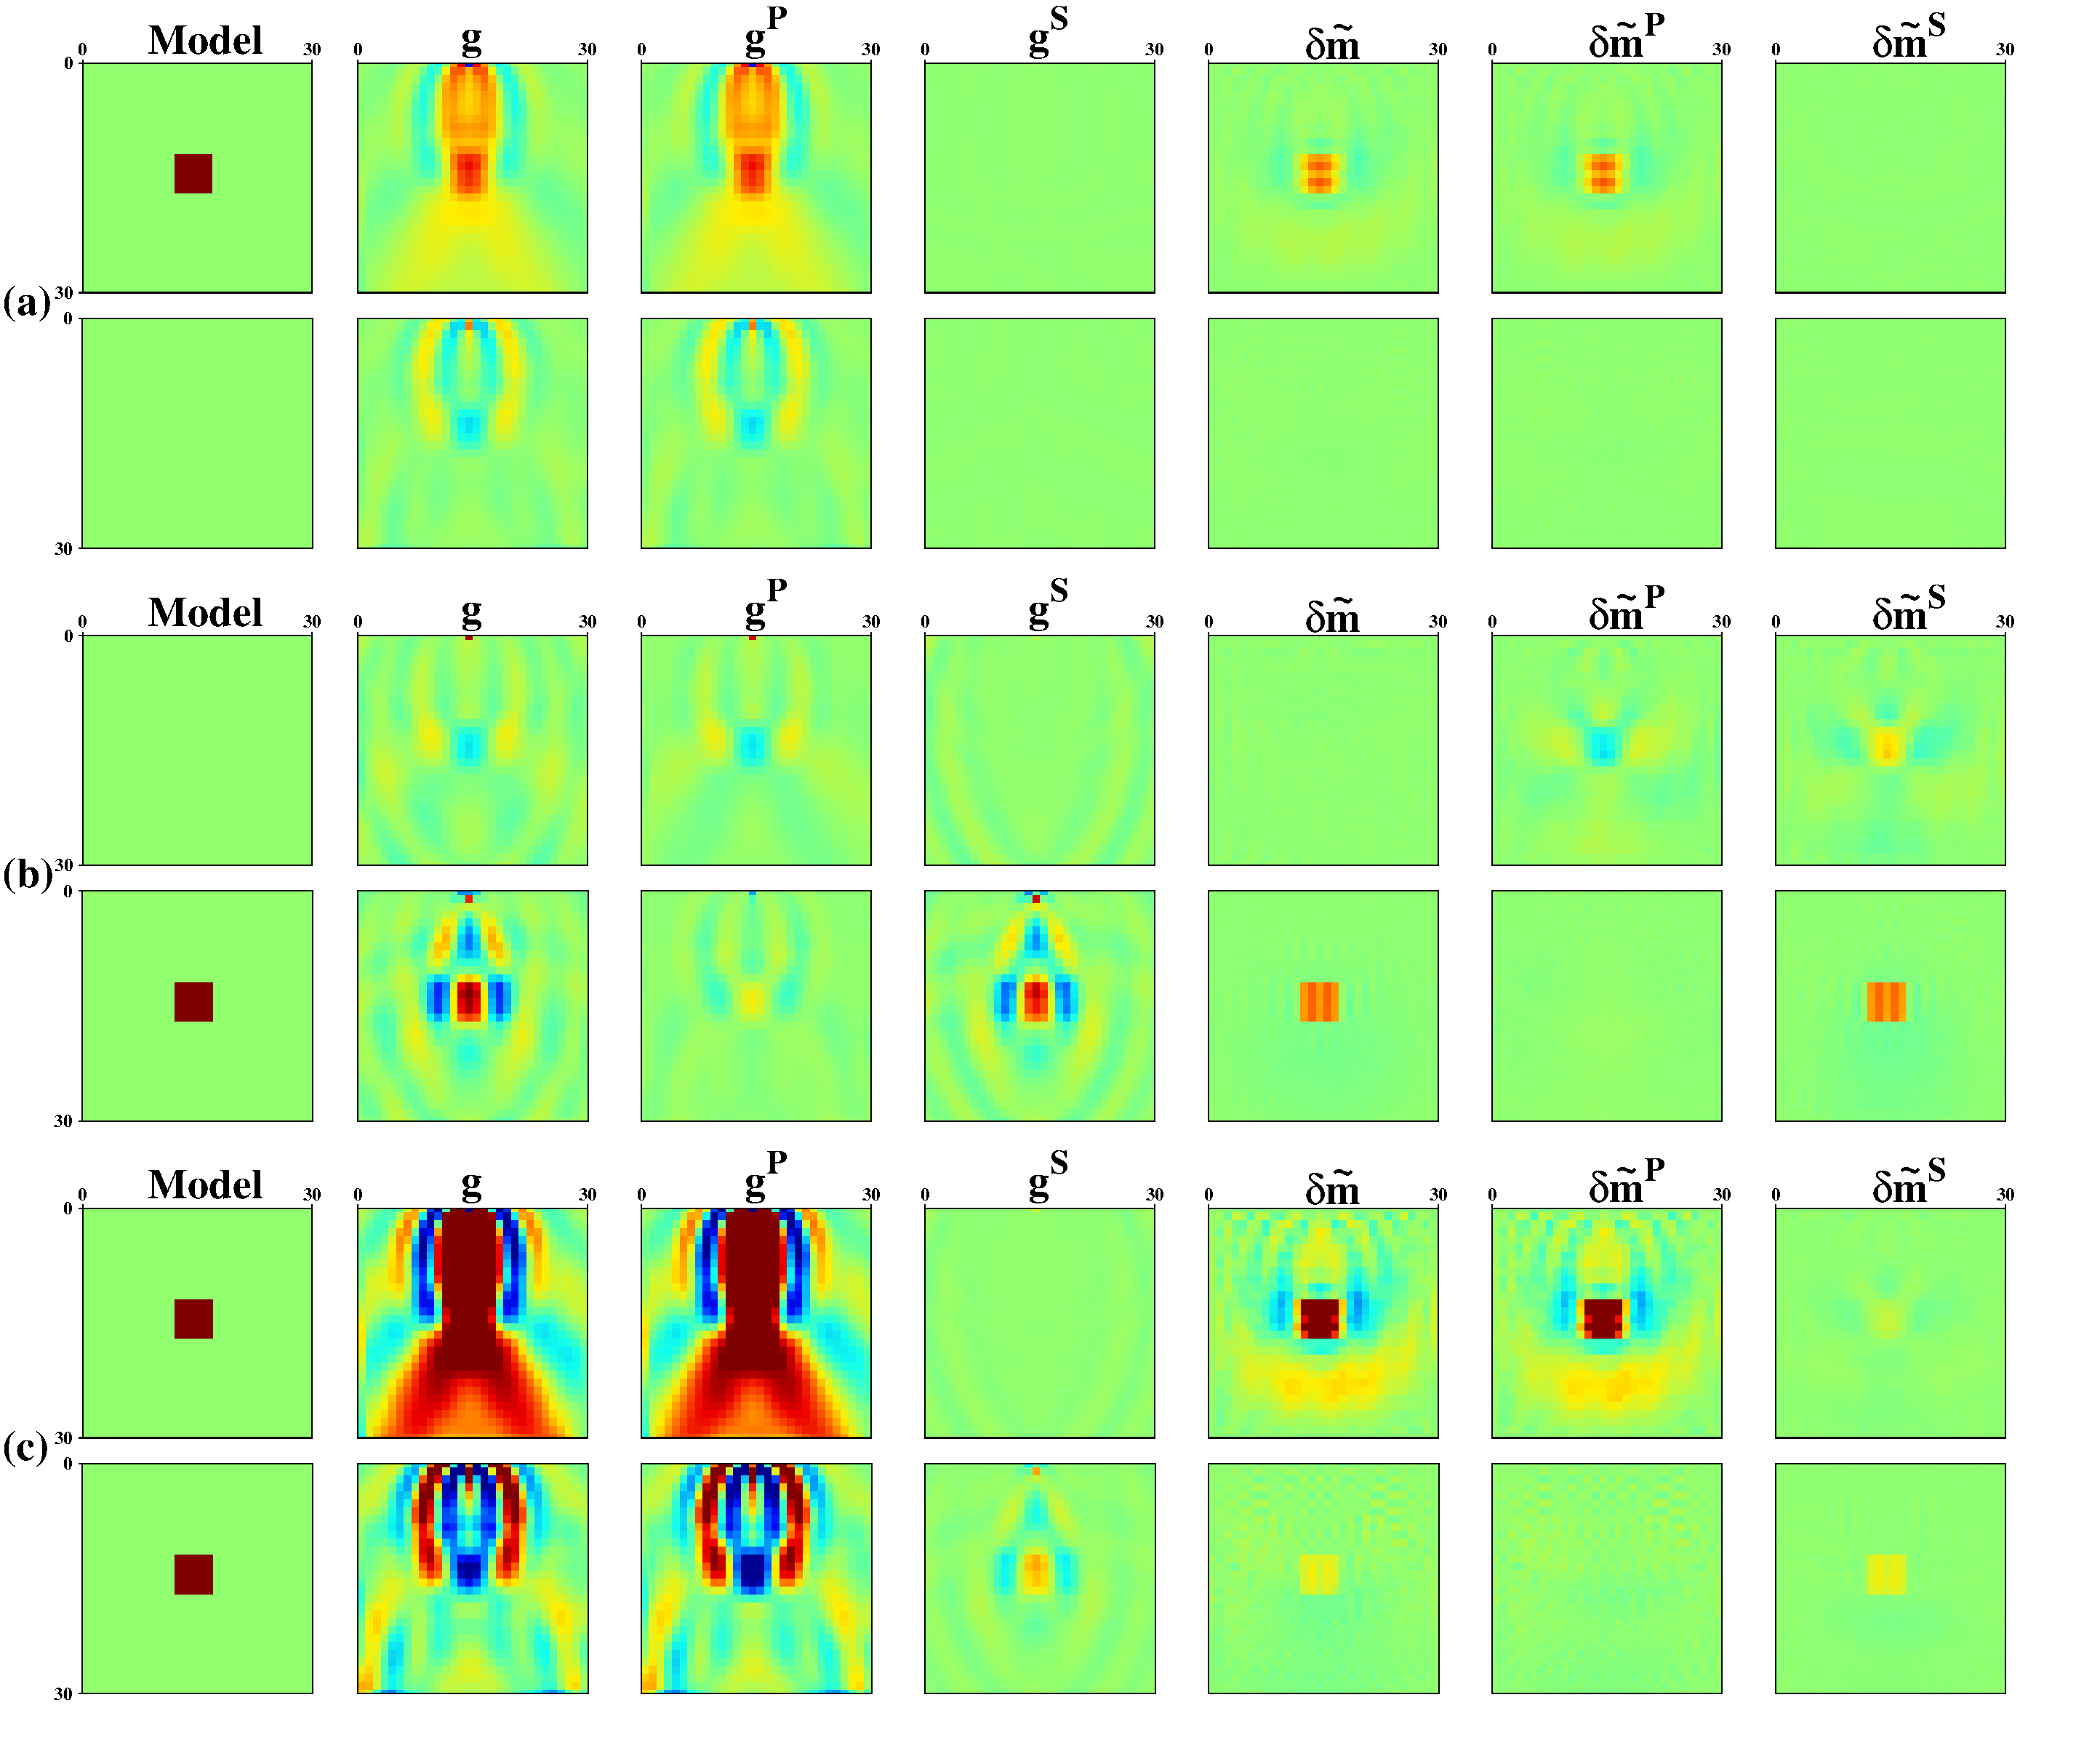
\includegraphics[width=14cm]{Figure/chapter02/Hessiantest/Fig/newepsall.pdf}
        \caption{
			常规(PCG)、模式解耦(MDPCG)和高斯-牛顿(GN)梯度对比:
    (a) $\delta V_p \neq 0$, $\delta V_s=0$; (b) $\delta V_p=0$, $\delta V_s\neq0$; and (c)
    $\delta V_p=10 \delta V_s$.
	从上到下为三个面板,每个面板中包含2行7列。第一行对应$V_p$,
	第二行对应$V_s$。7列从左到右依次为真实模型$\mathbf{m}=(\mathbf{V}_p,
    \mathbf{V}_s)$;
    PCG梯度$\mathbf{g}=(\mathbf{g}_{V_p},\mathbf{g}_{V_s})$,
    $\mathbf{g}^P=(\mathbf{g}^P_{V_p},\mathbf{g}^P_{V_s})$,
    $\mathbf{g^S}=(\mathbf{g}^S_{V_p},\mathbf{g}^S_{V_s})$;
    GN 梯度$\delta
    \tilde{\mathbf{m}}=(\delta\tilde{\mathbf{V}}_p,\delta\tilde{\mathbf{V}}_s)$;
        MDPCG梯度$\delta
        \tilde{\mathbf{m}}^P=(\delta\tilde{\mathbf{V}}^P_p,\delta\tilde{\mathbf{V}}^P_s)$
         $\delta
        \tilde{\mathbf{m}}^S=(\delta\tilde{\mathbf{V}}^S_p,\delta\tilde{\mathbf{V}}^S_s)$。
    }
    \label{fig:all}
    \end{center}
\end{figure}

在图\ref{fig:all}中,同样采用前文小模型实验来比较常规(PCG)、模式解耦(MDPCG)和高斯-牛顿(GN)第一次迭代的梯度。
在模型中央放置三种不同类型、尺度为10$\times$10m的参数扰动组合,分别为:(a) $\delta V_p \neq 0$, $\delta V_s = 0$; (b) $\delta V_p = 0$,
$\delta V_s \neq 0$和(c) $\delta V_p =10\delta
V_s$。初始模型为均匀的背景速度。在第一组实验中只有P波数据,可以看到原始的梯度($\mathbf{g}_{V_p}$和$\mathbf{g}_{V_s}$)中,有非常明显的参数耦合效应。
从图\ref{fig:all}a和b中可以看到,对于物理参数A而言,另一个参数B扰动会产生一个与B扰动方向相反的A的梯度。从图\ref{fig:all}b和c中$\mathbf{g}^{P}_{V_s}$看到,尽管P波数据残差可能携带了$\delta V_s$的信息,
常规梯度类方法用P波数据来反演$V_s$将会受到参数耦合的影响。在第三组实验中,由于参数耦合的影响,$\mathbf{g}^P_{V_s}$甚至提供了错误的更新方向。
由于S波残差只与$\delta
V_s$有关,因此正如我们所期望,$\mathbf{g}^S_{V_s}$总是能提供一个正确的更新方向。所以,$\mathbf{g}^P_{V_s}$是梯度中参数耦合部分的主导者。
一般来说,在以P波能量占主导的地震数据中,梯度中的这种耦合成分总是带来负面的影响,除非采用行之有效的预条件算子,例如图\ref{fig:all}中的GN梯度。

更重要的是,图\ref{fig:all}中最后三列在数值上验证了方程\eqref{eq:KeyPoint},同时也展示了MDPCG方法与GN方法之间的异同。与常规梯度法不同,
GN方法利用Hessian的逆以不同权重叠加三个解耦之后的梯度
($\mathbf{g}^P_{V_p}$、$\mathbf{g}^P_{V_s}$和$\mathbf{g}^S_{V_s}$),来实现P波速度梯度的最佳预条件。对于S波速度,GN方法实际上用
$\mathbf{G}$做为算子来对S波速度梯度($\mathbf{g}^S_{V_s}$)做预条件处理。算子$\mathbf{G}$近似等价于$[\mathbf{J}^{S}_{V_s}]^{\dagger}\mathbf{J}^{S}_{V_s}$的伪逆
(见方程\ref{eq:ResoOperS2})。正如方程\eqref{eq:Gradientmethod}所示,MDPCG方法也需要进一步的预条件来加速收敛。例如,预条件算子$\mathbf{Q}_2$
只需要考虑S波的照明补偿以及子波带宽效应即可,即近似$\mathbf{G}$的效果。因此,对
$V_s$反演,MDPCG方法几乎可看作是采用解耦的S波数据进行的单参数反演。相应地,预条件算子$\mathbf{Q}_2$要更廉价一些,比如利用单参数拟Hessian或者l-BFGS
方法。这种预条件方法为$V_s$反演近似提供了GN方法的梯度从而降低了迭代中的参数耦合,能够在不引入Hessian的情况下加速收敛。

\section{数值实验}
本节用两个理论合成数据的例子来验证模式解耦EFWI的有效性。实验中采用纯P波震源来合成多分量地震记录。
从较好的初始模型开始,$V_p$和$V_s$将同时被反演。在时间域对数据进行低通滤波,然后采用从低频到高频的多尺度策略来避免陷入局部极值。反演
分为四个不同的阶段:0-2Hz,0-4Hz,0-6Hz和0-10Hz。整个数值实验中,采用原始梯度的PCG与采用模式解耦梯度的MDPCG法都使用了随深度变化的照明补偿算子来进行预条件\cite[]{kohn:2012}。
\subsection{流体饱和模型}
图\ref{fig:smallmodel}定义了一个在砂岩背景模型中的流体饱和储层,背景模型参数为$V_p=3.14 km/s$, $V_s=1.56 km/s$以及$\rho=2000 kg/m^{-3}$。储层的上部含气饱和,参数为
$V_p=2.6 km/s$和$V_s=1.66 km/s$,下部含水,$V_p=3.0 km/s$和$V_s=1.66 km/s$。
储层的速度值根据砂岩岩石物理模型给出\cite[]{mavko2009rock}。在模型顶部放置炮点和检波器,合成32炮数据,炮间距为100m,每炮数据为400道记录,道间距为10m。反演以背景模型作为初始模型。
每阶段最大迭代次数限制为10次。从反演结果上看,常规EFWI方法能得到可接受的$V_p$模型,而$V_s$反演结果受参数耦合影响则非常糟糕。
这是因为在初始阶段,梯度会受到参数耦合的强烈影响,导致模型中长波长成分的重建受到严重干扰,因此在有限的迭代次数下反演最终收敛到了局部极值。
采用了MDPCG之后,EFWI最后很好地重建了$V_p$和$V_s$模型。
\begin{figure}[!htb]
    \begin{center}
		\subfloat[]{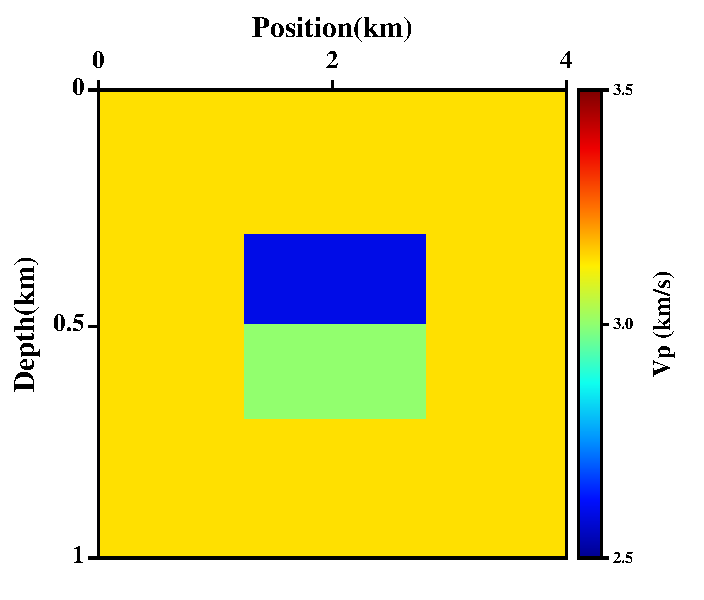
\includegraphics[width=5cm]{Figure/chapter02/smallmodel/Fig/truevp.pdf}}
		\subfloat[]{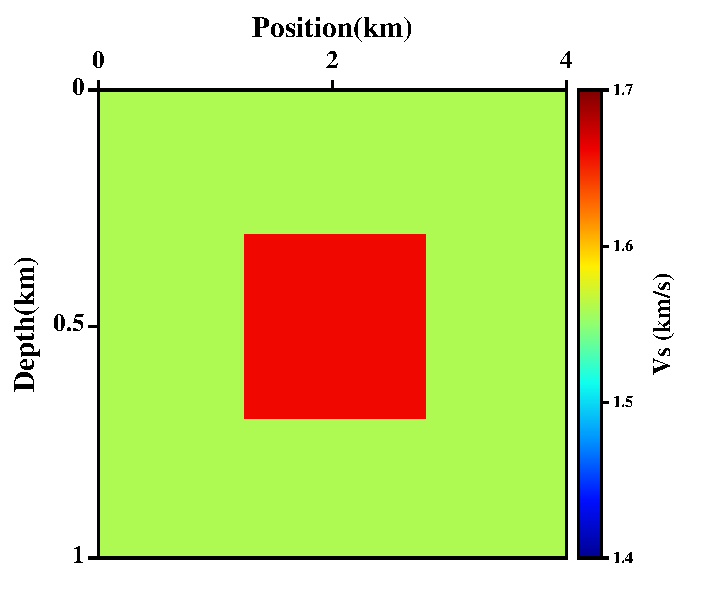
\includegraphics[width=5cm]{Figure/chapter02/smallmodel/Fig/truevs.pdf}}\\
		\subfloat[]{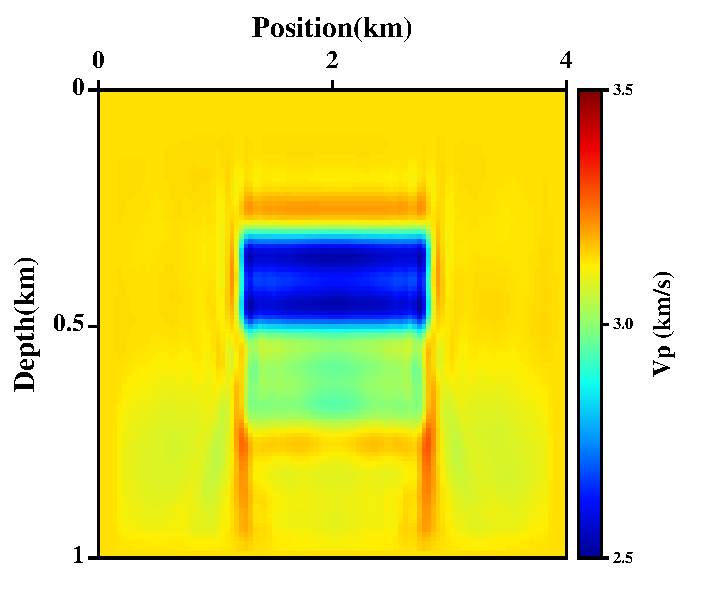
\includegraphics[width=5cm]{Figure/chapter02/smallmodel/Fig/nodecomvp.pdf}}
		\subfloat[]{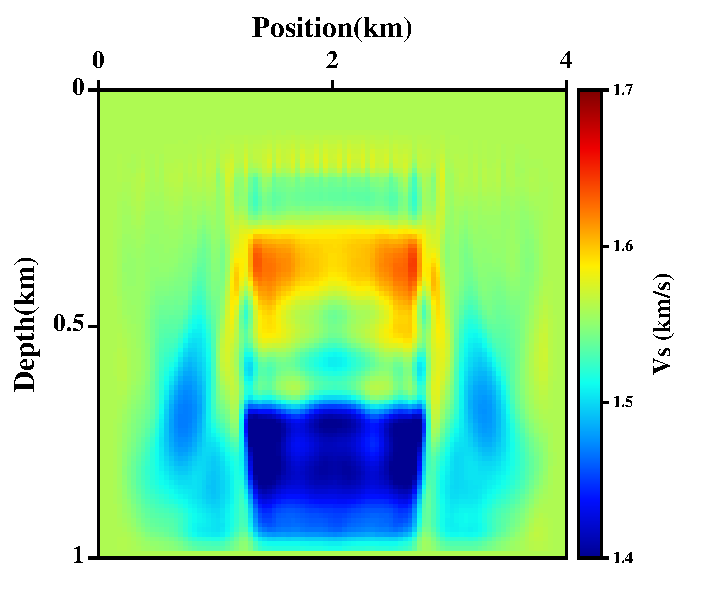
\includegraphics[width=5cm]{Figure/chapter02/smallmodel/Fig/nodecomvs.pdf}}\\
		\subfloat[]{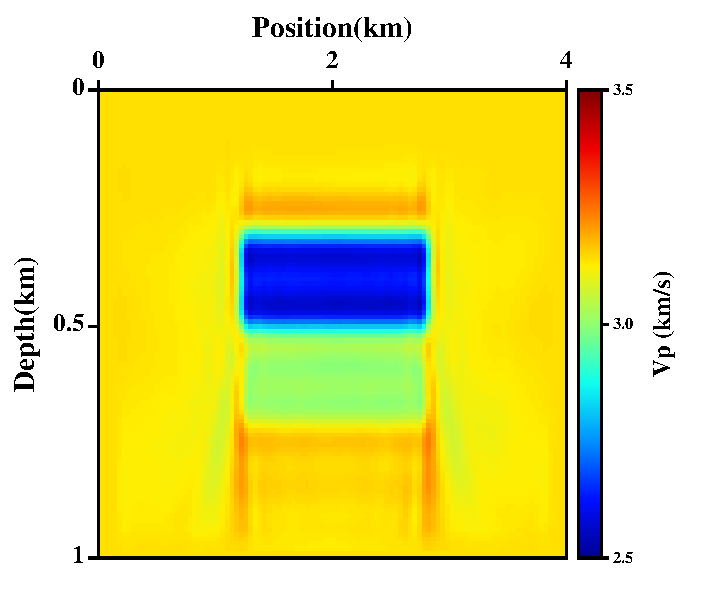
\includegraphics[width=5cm]{Figure/chapter02/smallmodel/Fig/decomvp.pdf}}
		\subfloat[]{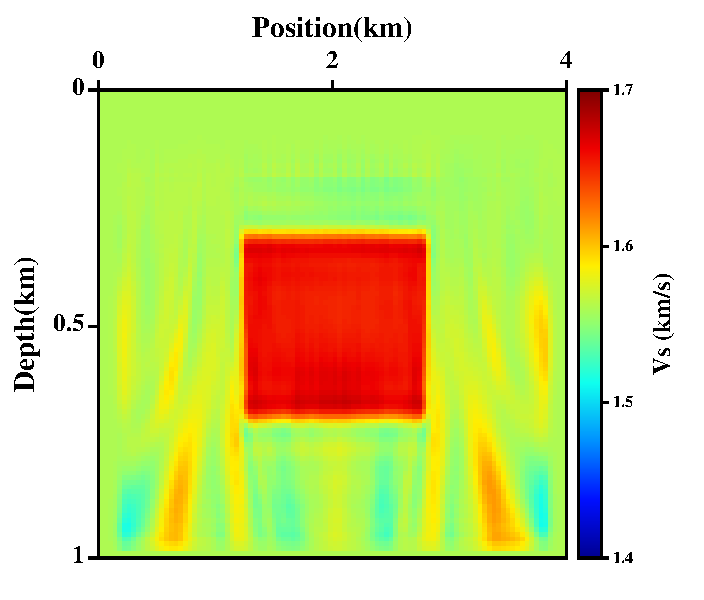
\includegraphics[width=5cm]{Figure/chapter02/smallmodel/Fig/decomvs.pdf}}
        \caption{
			流体饱和砂岩模型的EFWI结果:左侧为$V_p$,右侧为$V_s$;
			(a),(b)为真实模型;(c),(d)为常规PCG方法反演结果; (e), (f)为MDPCG方法反演结果。
    }
    \label{fig:smallmodel}
    \end{center}
\end{figure}
\subsection{Marmousi-II模型}
\begin{figure}[!htb]
    \begin{center}
		\subfloat[]{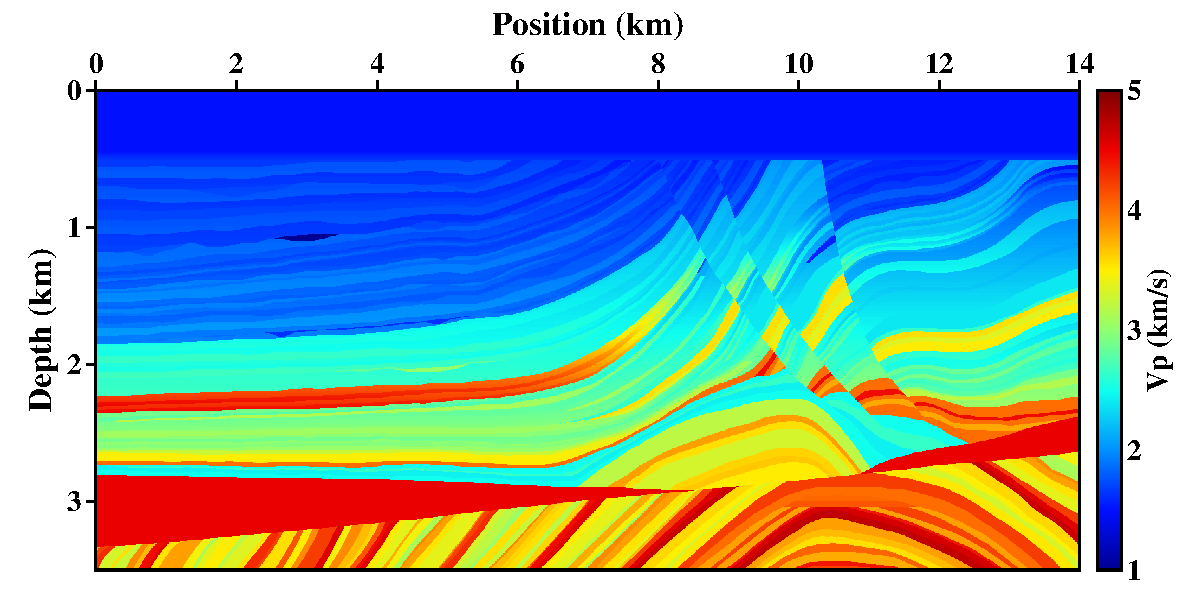
\includegraphics[width=7cm]{Figure/chapter02/tariqsugresult/Fig/truevp.pdf}}
		\subfloat[]{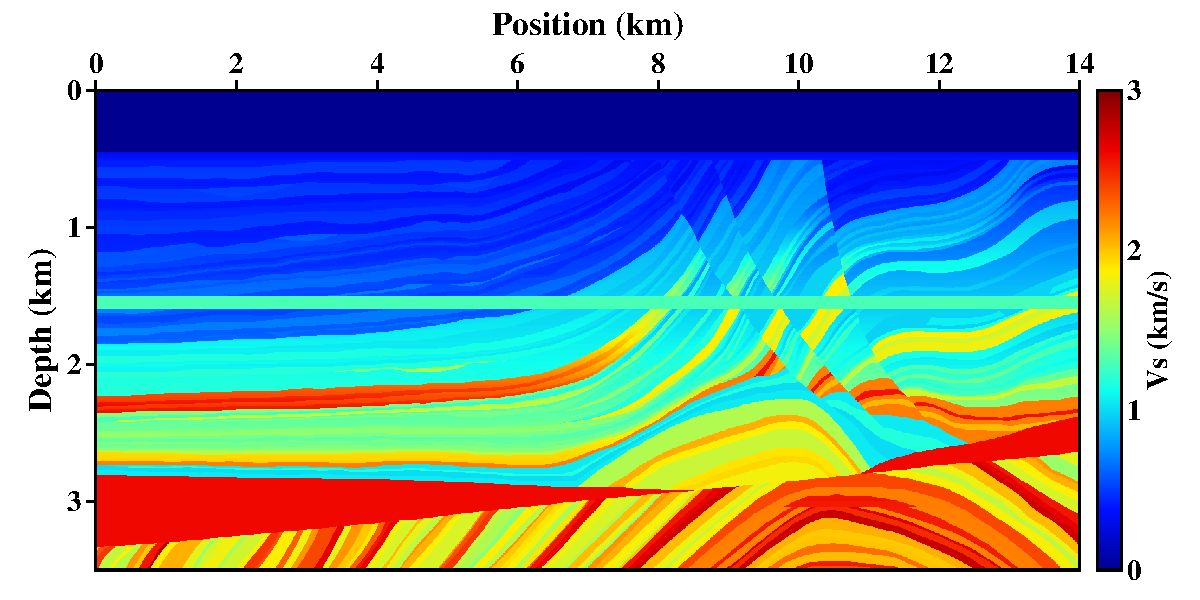
\includegraphics[width=7cm]{Figure/chapter02/tariqsugresult/Fig/truevs.pdf}}\\
		\subfloat[]{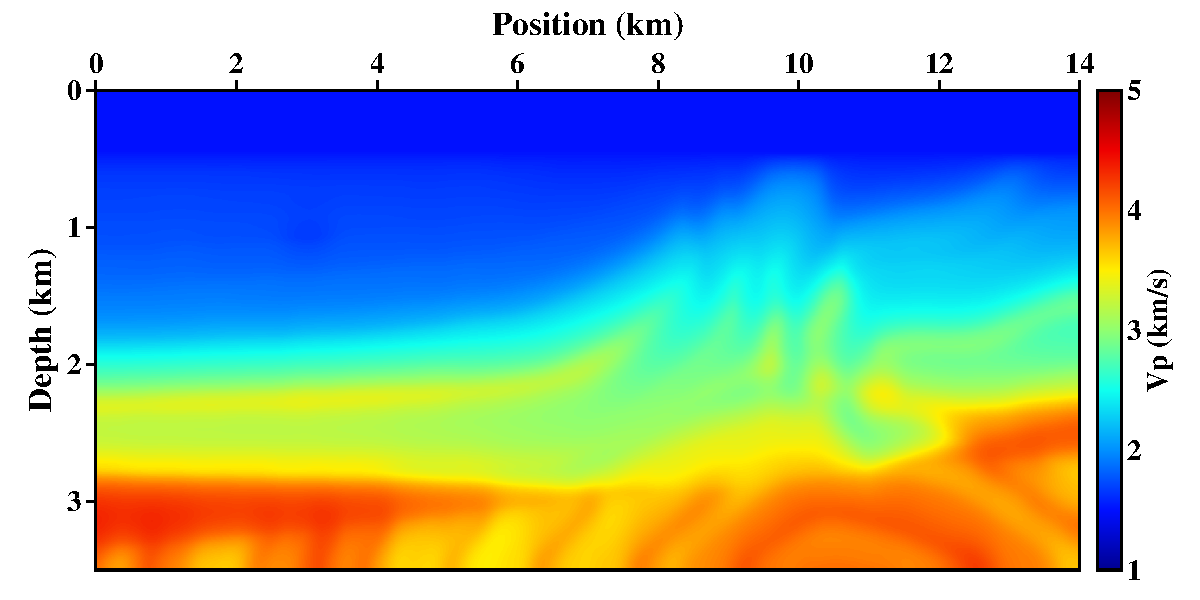
\includegraphics[width=7cm]{Figure/chapter02/tariqsugresult/Fig/initvp.pdf}}
		\subfloat[]{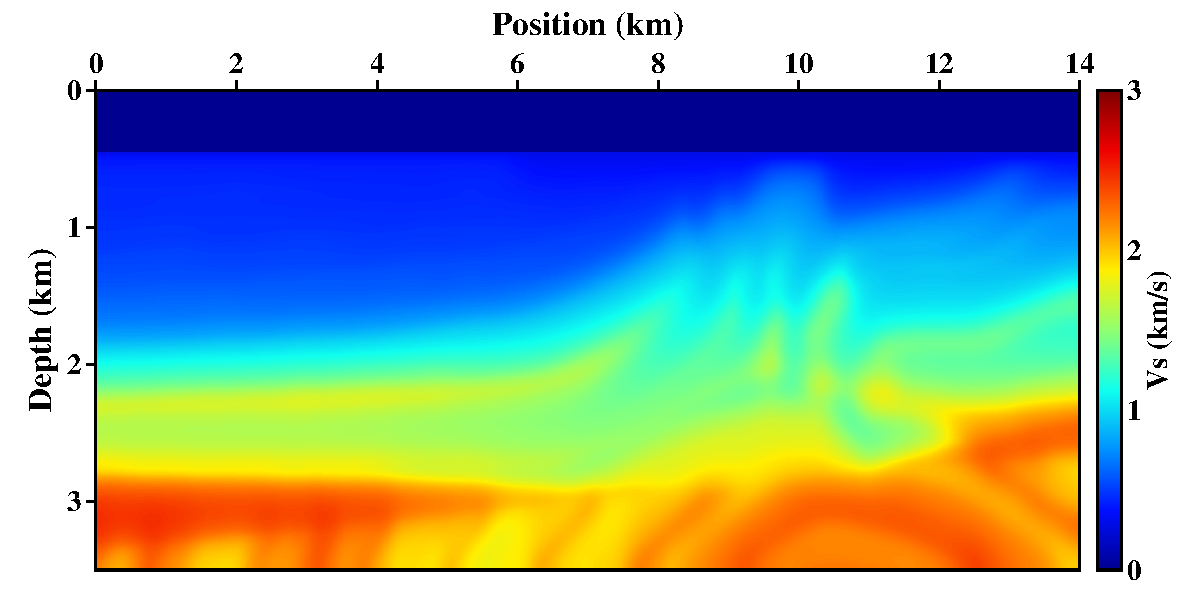
\includegraphics[width=7cm]{Figure/chapter02/tariqsugresult/Fig/initvs.pdf}}
        \caption{
			SEG Marmousii-II模型:(a), (b)分别为真实的$V_p$和$V_s$模型; (c),
			(d)分别为初始的$V_p$和$V_s$模型。注意,P波速度含有含气沙岩储层产生的速度异常以及S波速度
			中加入了高速薄层异常结构。
    }
    \label{fig:MarInitTrue}
    \end{center}
\end{figure}
\begin{figure}[!htb]
    \begin{center}
		\subfloat[]{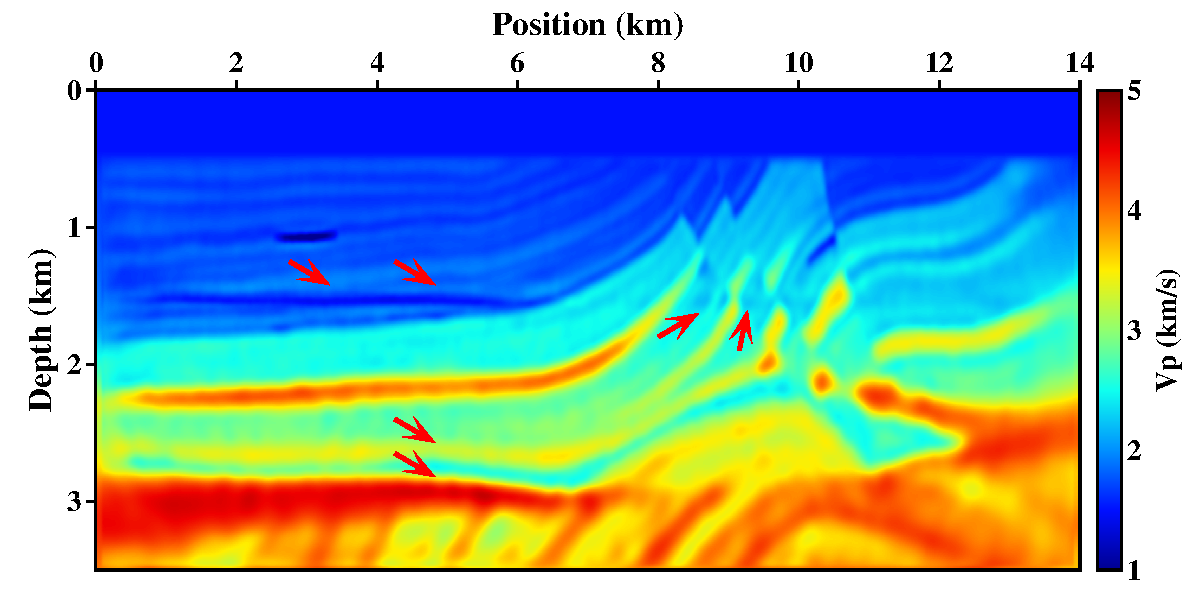
\includegraphics[width=7cm]{Figure/chapter02/tariqsugresult/Fig/nodevp.pdf}}
		\subfloat[]{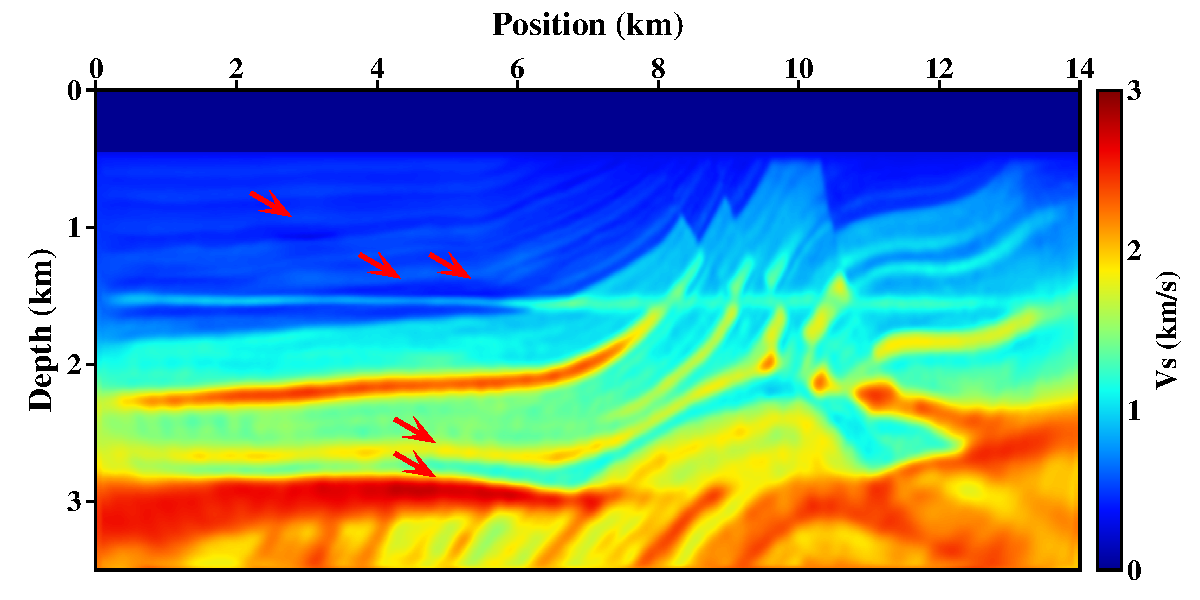
\includegraphics[width=7cm]{Figure/chapter02/tariqsugresult/Fig/nodevs.pdf}}\\
		\subfloat[]{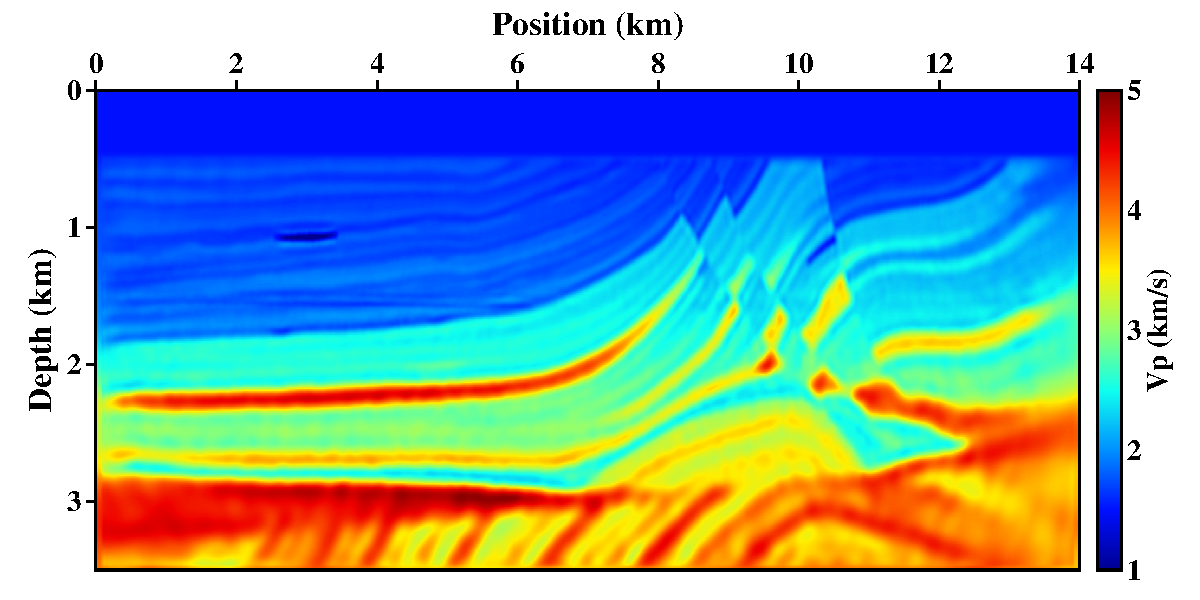
\includegraphics[width=7cm]{Figure/chapter02/tariqsugresult/Fig/devp.pdf}}
		\subfloat[]{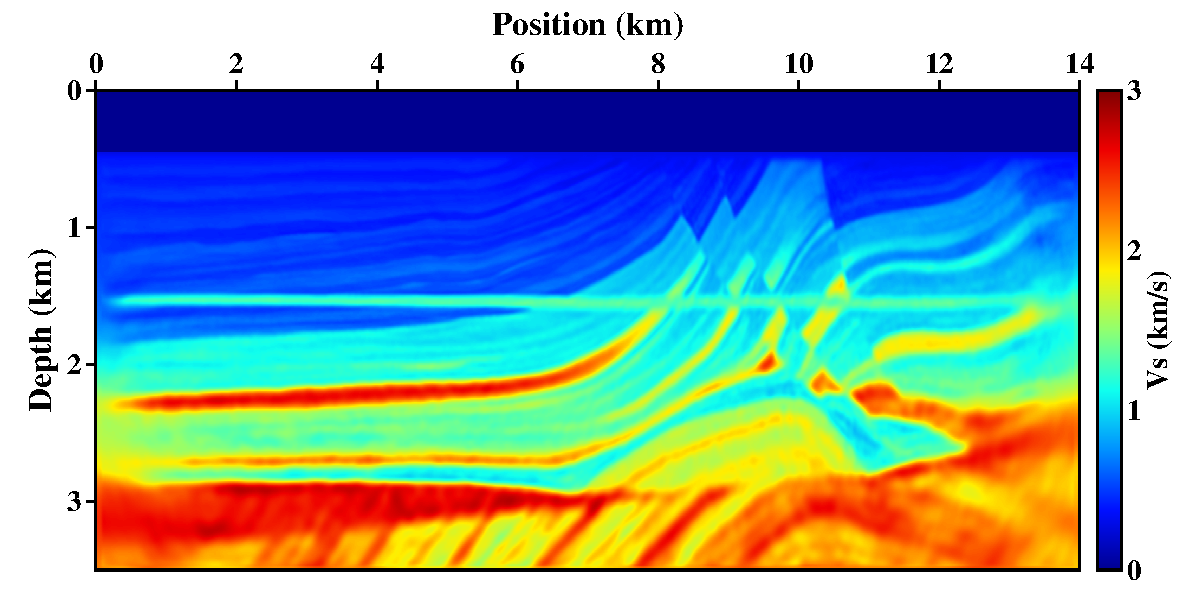
\includegraphics[width=7cm]{Figure/chapter02/tariqsugresult/Fig/devs.pdf}}
        \caption{
			反演的Marmousi-II模型:其中左侧为$V_p$,右侧为$V_s$. (a), (b)为常规PCG方法反演结果;(c), (d)为MDPCG方法反演结果。
%        The inverted Marmousi-II model: The inverted results using the PCG (a, b)
%            and the MD-based methods (c, d).
%        (a) and (c) are $V_p$ models while (b) and (d) are $V_s$ models.
    }
    \label{fig:MarInvert}
    \end{center}
\end{figure}
过去十年间,很多EFWI策略被用在了OBC地震数据中。在地震数据低频成分比较丰富的情况下,重建低Poisson比的模型(如硬海底)相对比较容易\cite[]{bae:2012}。
然而,软海底环境在现实中更为普遍。此时,PS转换能量非常有限,反演中的非线性程度以及参数间的耦合也
会变得更加严重。为了应对这种更真实的软海底情况,
如图\ref{fig:MarInitTrue}(a)和(b)所示,采用泊松比变化剧烈的原始Marmousi-II模型测试算法。不同参数间非一致的结构能更明显地调查参数间的耦合程度。
为了更好的展示本文方法的优势,在S波速度模型1.5km深处添加了一个高速的薄层。在反演中,采用交错网格有限差分法来计算正传与伴随波场,空间采样间隔为5m,
记录总时间为8s,时间采样间隔为0.5ms。共有40炮合成数据,炮点深度在20m的水深处,2800个检波点放置于海底来模拟OBC观测。初始模型通过SU软件中的smooth2函数
平滑真实模型产生,平滑半径为300m。采用与前一实验同样的多尺度策略,但是每阶段最大迭代次数扩大为40次。

图\ref{fig:MarInvert}的结果表明了MDPCG方法比常规PCG方法能提供更好的反演结果。
在模型浅部(约1.5km),两种方法都能很好的恢复$V_p$模型,而常规方法恢复的$V_s$模型
分辨率较低。S波速度模型中的高速异常薄层给反演造成了很大的挑战,如图\ref{fig:MarInvert}(a)和(b)中所示,反演结果存在很强的参数耦合
的干扰,尤其是在左侧的高速异常薄层附近。这就导致了该异常薄层下方构造的错位与不聚焦(如图中箭头所示)。然而,MDPCG方法很好地压制了这些参数耦合效应,
获得了模型的许多细节,包括中部的断层与背斜构造。模型的纵向“测井”曲线(图\ref{fig:VertiProfile})
进一步证明了模式解耦反演方法获得了比常规方法更准确的结果与更高的分辨率。
\begin{figure}[!htb]
	\begin{center}
		{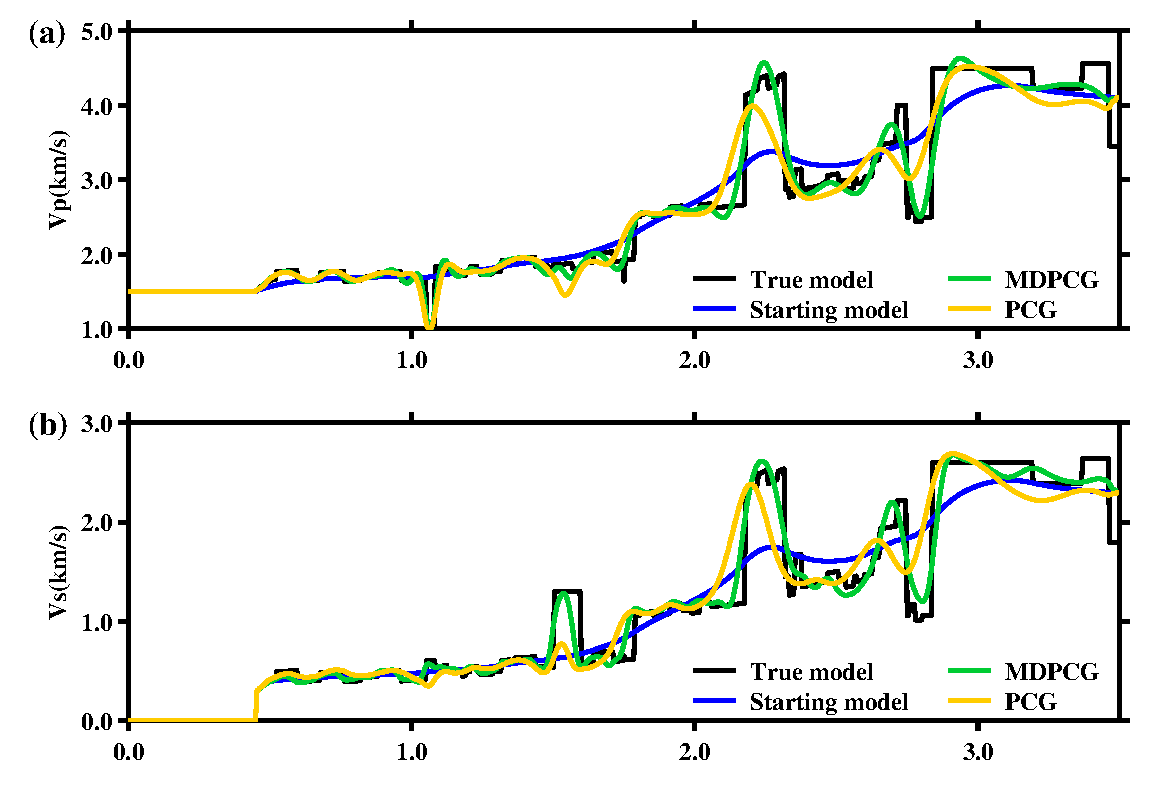
\includegraphics[width=10cm]{Figure/chapter02/tariqsugresult/Fig/new3km.pdf}}
		{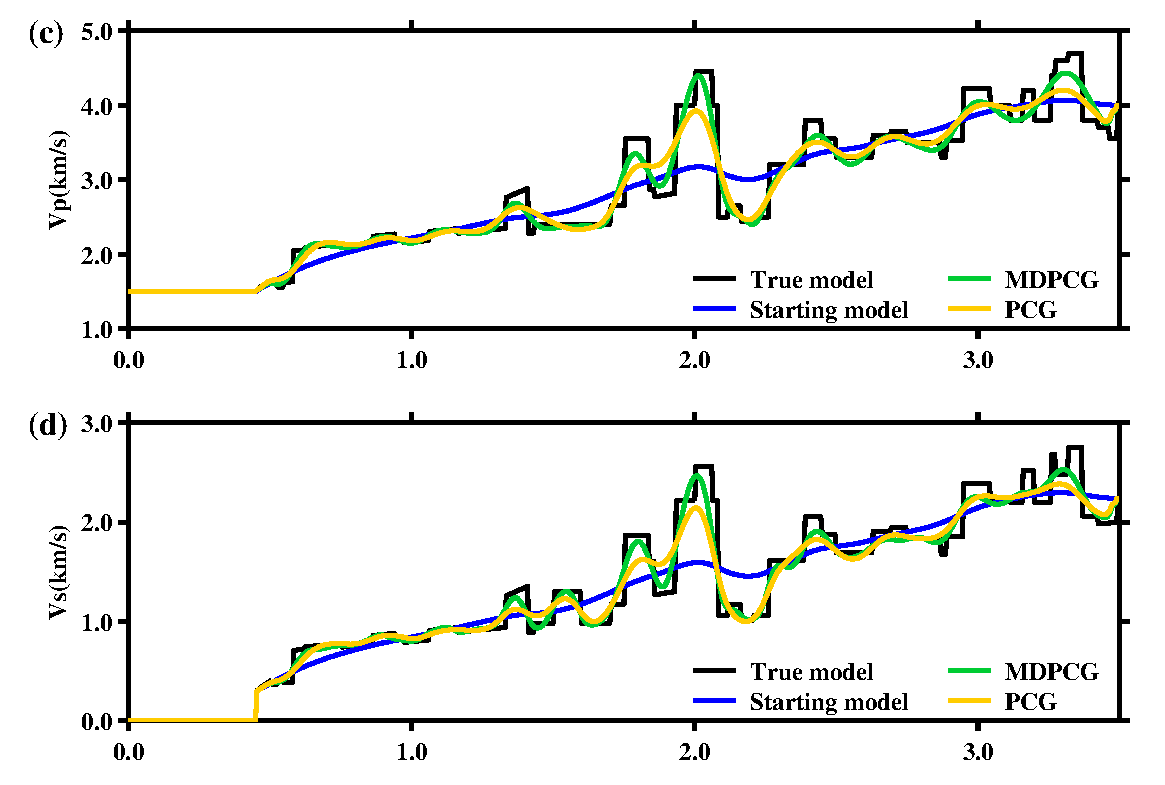
\includegraphics[width=10cm]{Figure/chapter02/tariqsugresult/Fig/new9km.pdf}}
		\caption{
		模型在3.0km(a,b)和9.0km(c,d)处的纵向剖面。黑线和蓝线分别代表真实和初始模型;黄线与绿线分别代表常规PCG和MDPCG方法反演结果。
%		The velocity profiles at 3.0 km (a, b) and 9.0 km (c, d) with the true models
%			(black),
%			the initial models (blue), the PCG-based (yellow) and MD-based (green)
%			inverted models.
	}
	\label{fig:VertiProfile}
	\end{center}
\end{figure}

\begin{figure}[!htb]
    \begin{center}
        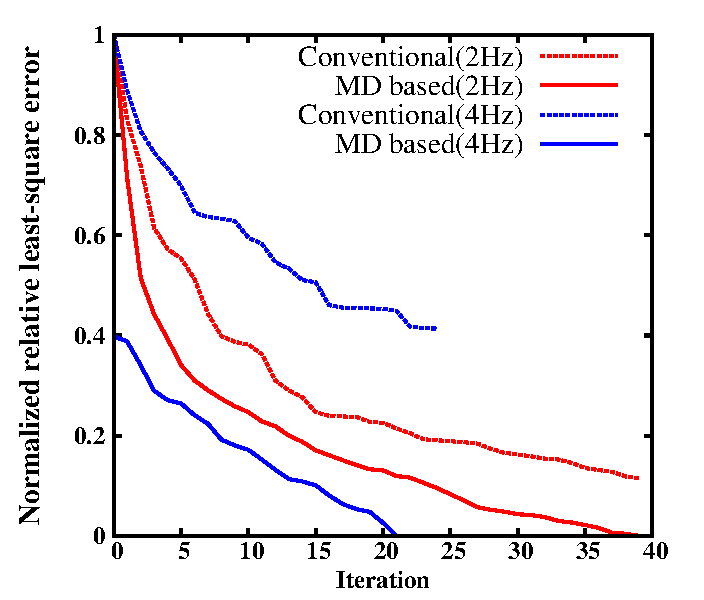
\includegraphics[width=10cm]{Figure/chapter02/tariqsugresult/Fig/L2.pdf}
        \caption{
			归一化后的L2残差随迭代次数的变化。红色与蓝色代表第一和第二阶段的反演,虚线代表常规PCG方法
			实线代表MDPCG方法。
%            Normalized L2 norms as a function of iteration for the PCG-based (dash)
%            and MD-based (solid) inversions in the first (red) and second (blue)
%            stages.
    }
    \label{fig:L2}
    \end{center}
\end{figure}
图\ref{fig:L2}展示了在前两个阶段的反演中,归一化的目标函数值随迭代次数的下降曲线。可以看到,MDPCG方法要比常规PCG方法收敛更快。在第一个阶段,模式解耦
反演方法的数据拟合程度更高,反演结果恢复了更准确的中低波数成分。在第二个阶段,常规PCG方法最终在25次迭代之后停止更新且数据残差仍相当大,而MDPCG方法
在22次迭代后数据残差快速下降达到终止条件。这些分析表明利用模式解耦对梯度做预条件可以很有效地在反演中降低参数耦合从而加速收敛。

表\ref{table:TotalComputime}
中列出了在8节点(每节点15核)的工作站上每个阶段的迭代次数和总的计算时间。每个阶段我们设定最大迭代次数为40次。因为当搜索不到合适步长的时候迭代会自动终止,所以
不同阶段的实际迭代次数并不相同。在常规方法中,严重的参数耦合效应会影响从低频数据中重建出合适的宏观模型,这就导致在高频阶段无法获得合理的梯度方向,使得迭代过早终止。而MDPCG方法可以一定程度压制参数耦合,在低频阶段能够重建出合适的宏观模型,从而使得高频阶段的梯度更合理。这也是为什么模式解耦方法能
获得更准确、分辨率更高的反演结果。总的来说,模式解耦方法需要更多的迭代次数,也因此耗费更多计算时间。就本例而言每次迭代的平均用时只增加了18\%左右。
\begin{table}[!htb]
    \caption{计算时间对比}
    \label{table:TotalComputime}
	\centering 
%   \begin{tabular}{|c|c|c|c|c|c|c|}
%   \begin{tabular}{|p{1.8cm}|c|c|c|c|p{2.2cm}p{2.3cm}p{2cm}|}
    \begin{tabular}{p{1.8cm}p{1.0cm}p{1.0cm}p{1.0cm}p{1.2cm}p{1.0cm}p{1.0cm}}
%    \begin{tabular}{|p{1.8cm}|p{1.0cm}p{1.0cm}p{1.0cm}p{1.2cm}|p{1.0cm}p{1.0cm}|}
    \hline
    \quad&\multicolumn{4}{c}{Iteration number}&\multicolumn{2}{c}{Time spent (hour)} \\
%   \quad&\multicolumn{4}{|c|}{Iteration number}&\multicolumn{2}{|c|}{Computing Time (hour)} \\
    \hline
%   Method & stage1 0-2Hz &stage2 0-4Hz&stage3 0-6Hz&stage4 0-10Hz&Total &Average \\
    \multirow{2}{*}{Method} & stage1 &stage2 &stage3 &stage4 &\multirow{2}{*}{Total}
    &\multirow{2}{*}{Average} \\
    & 0-2Hz &0-4Hz&0-6Hz&0-10Hz\\
    \hline
    Conventional&  40   &25&5& 7  &41.4&0.538\\
    MD-based &   40  & 22 &33 &13&68.3&0.632\\
    \hline
    \end{tabular}
\end{table}
\section{讨论}
\subsection{更进一步分解梯度的必要性}
理论上讲,可以对正传与反传波场分别解耦从而获得不同模式转换(也即PP、PS、SP和SS)对应的解耦梯度。但是,很难设计出一个单独使用某一模式转换数据的EFWI方法,因为地面
P/S分离算法无法区分入射波场的类型,即无法区分PP与SP(或PS与SS)。或者只能使用分解后的单模式地震数据来进行单参数反演。例如
Ren和Liu\cite{ren.liu:2016},在其四步反演策略的第二步中,当有很强的S波能量时,只采用分解的P波场来反演P波速度,或者在弱S波能量时仅仅拟合S波数据来反演S波速度。


需要注意的是,在梯度计算中正传波场解耦等价于次级源(或背景波场)的波模式解耦,而次级源又是Frech{$\acute{e}$}t导数中的一部分。因此可以将该线性问题写为:
\begin{equation}
    \mathbf{J}^{XY}\delta\mathbf{m}=\mathbf{\delta u}^{XY},
    \label{eq:JXY}
\end{equation}
其中$X$和$Y$分别表示次级源与散射Green函数的波模式,$\mathbf{\delta u}^{XY}$则表示${X}{Y}$模式的扰动波场。根据方程\eqref{eq:ResoOperP}的推导方式,
可以获得相应的分辨率矩阵:
\begin{equation}
    \mathbf{R}^{XY}=\mathbf{H}_a^{-g}\mathbf{J}^{\dagger}\mathbf{J}^{XY}. 
    \label{eq:RXY}  
\end{equation}
图\ref{fig:ResoMN}展示了PP、PS、SP和SS模式的分辨率矩阵,其观测系统与图\ref{fig:Resolution}中一致,但是采用了P和S波的混合震源。由于更加复杂的
波现象,图中分辨率矩阵的对角带更宽。可以看到,$\mathbf{R}^{PP}$ 与$\mathbf{R}^P$十分类似,而$\mathbf{R}^{SP}$却几乎为空矩阵。这表明用PP波数据来反演$V_p$会受到来自$V_s$的干扰。而SP波数据
则对两个参数的反演贡献都很小。从Ren and Liu (2016)\cite{ren.liu:2016}的例子中(见其文中图19与20)可看到
,即使震源中含有足够强的S波能量,SP梯度也很弱且有很多噪音。一个
可能的解释就是如图\ref{fig:SPSS}所示,SP的散射能量很弱。此外,也难以
区分出PS和SS模式各自的贡献,因为从图\ref{fig:ResoMN}中看到,$\mathbf{R}^{PS}$和
$\mathbf{R}^{SS}$的非零元素分布非常一致,也就是说它们的分辨能力相似。因此,通过正传波场解耦来进一步压制参数耦合效应的潜力非常有限,尽管这样会带来更多的计算量。这也是为什么本文只
分解反传波场来对梯度进行预条件。
\begin{figure}[!htb]
    \begin{center}
        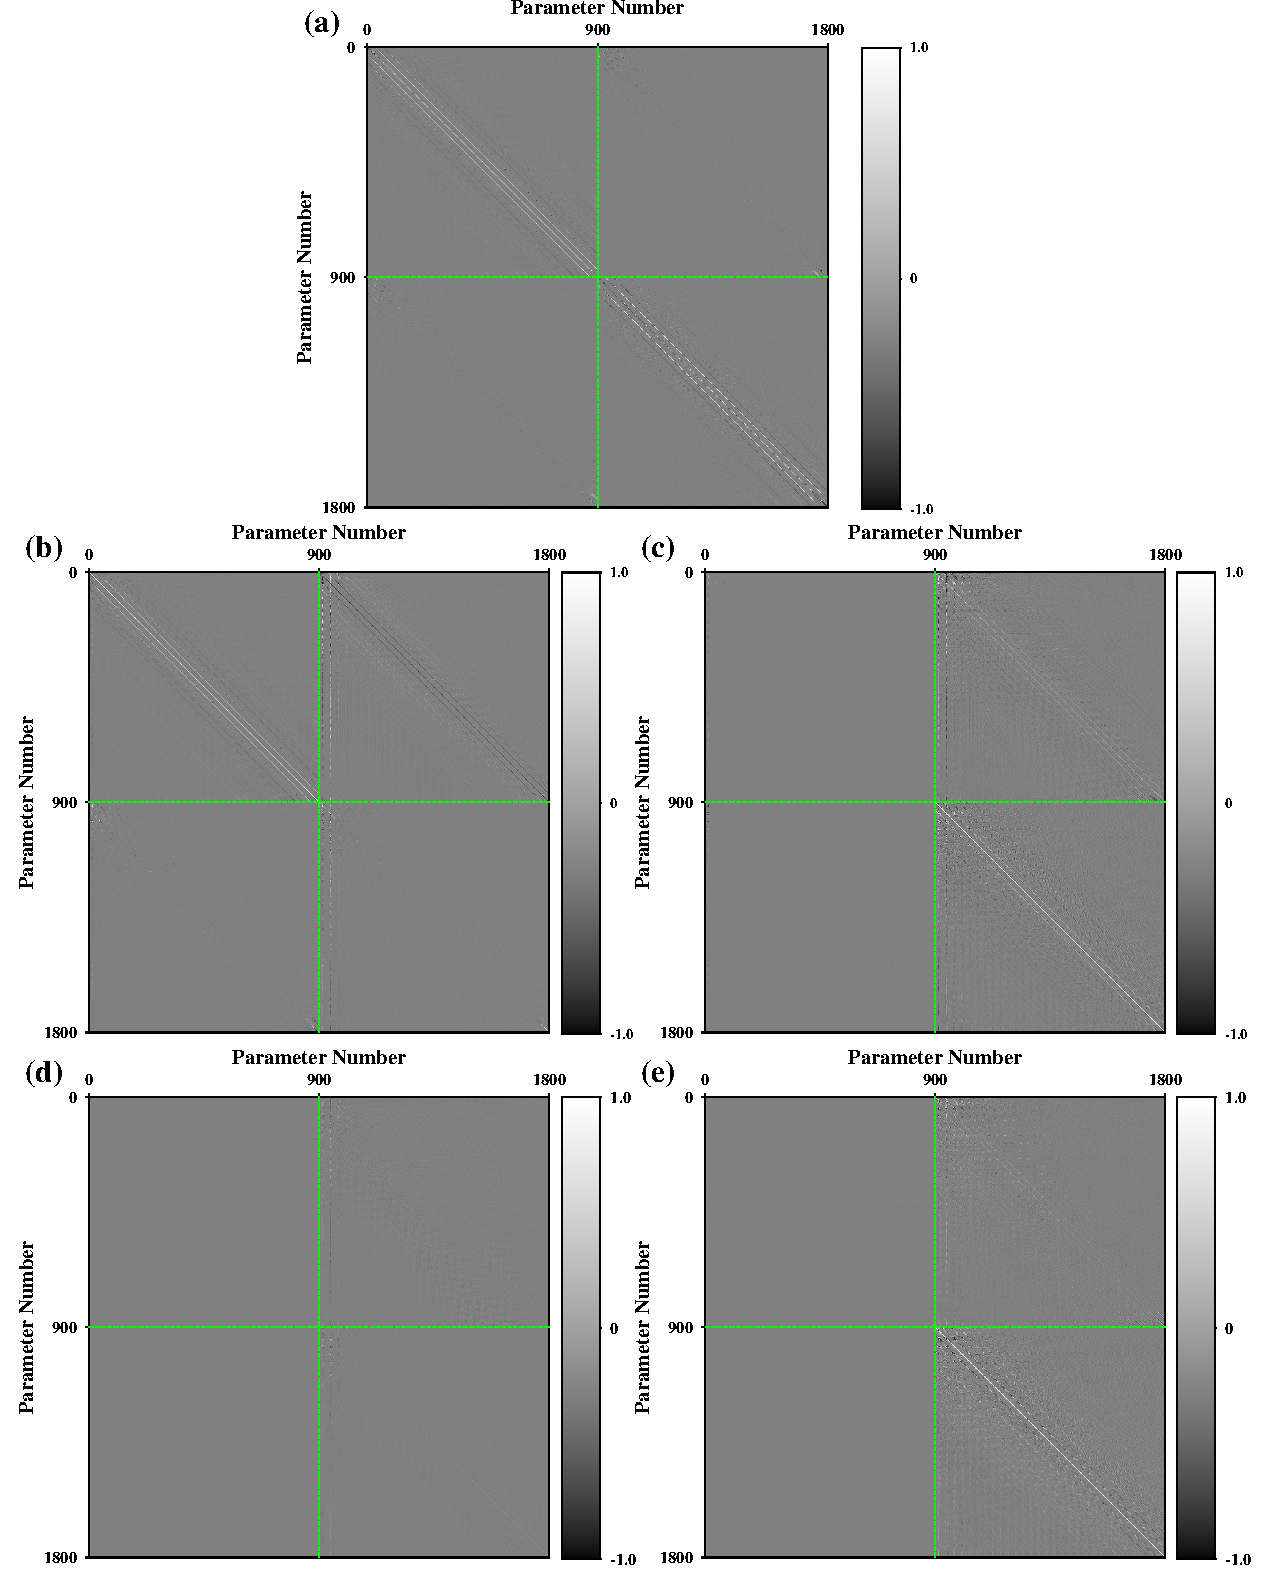
\includegraphics[width=12cm]{Figure/chapter02/ResoOpera/Fig/resolutionMN.pdf}
        \caption{
			采用混合震源时不同模式数据转换的分辨率矩阵。
%            Resolution matrices associated with different mode conversion data using
%            mix-source:
            (a) $\mathbf{R}$, (b) $\mathbf{R}^{PP}$, (c) $\mathbf{R}^{PS}$, (d)
            $\mathbf{R}^{SP}$ 和(e)
            $\mathbf{R}^{SS}$.
    }
    \label{fig:ResoMN}
    \end{center}
\end{figure}

\begin{figure}[!htb]
    \begin{center}
        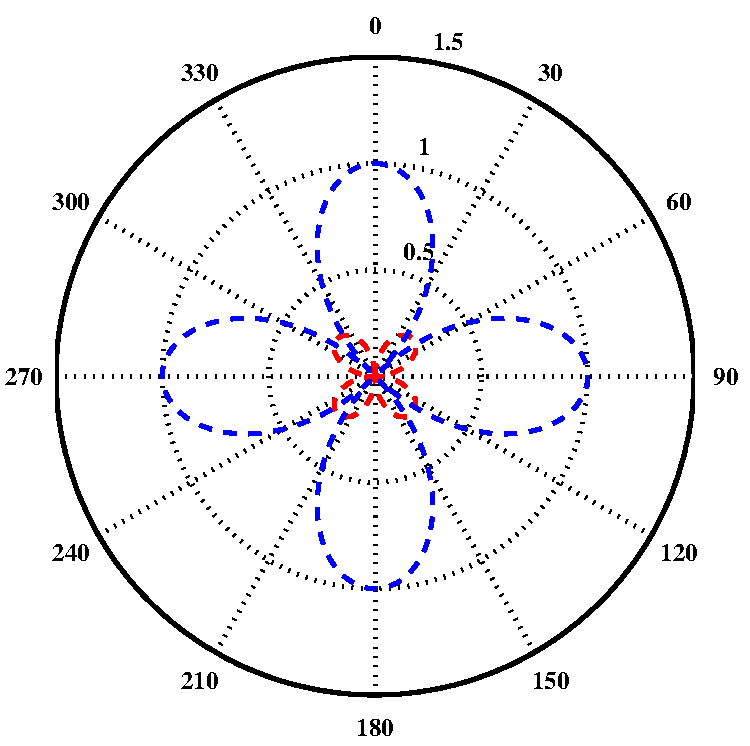
\includegraphics[width=6cm]{Figure/chapter02/radiationpattern/Fig/SPSS.pdf}
        \caption{
			归一化的SP模式(红色)和SS模式(蓝色)的辐射模式。
%            Radiation pattern of SP and SS modes with a same normalization: SP
%            mode (red) and SS mode (blue).
    }
    \label{fig:SPSS}
    \end{center}
\end{figure}
\subsection{密度模型的反演}
密度扰动同时散射P和S波,但是却几乎不影响两种波模式的相位或者走时。这些模式的散射能量大多与入射波场的传播方向相反\cite[]{wu.aki:1985,tarantola:1986}。因此,
密度作为一个次级效应参数,由于其微弱的敏感性和多参数的耦合效应\cite[]{tarantola:1986,forgues.lambare:1997},很难被准确重构。这也是为何很多EFWI的研究只考虑
常密度的情形\cite[]{shipp:2002,sears2008,brossier2009}。只有很少一部分的工作能够利用多尺度策略和(或)不同参数化方式的选取中获得较为合理的密度反演结果
\cite{jeong2012full}。最近,基于子空间方法\cite[]{kennett:1988},Xu and McMechan\cite{xu.mcmechan:2014}提出了一种多步长的梯度类方法来压制$V_p$, $V_s$和
$\rho$之间的串扰。Yang et al.
(2016)\cite{Yang2016}采用改进的散射积分法(SI)通过Hessian信息来改善声波FWI中$V_p$和$\rho$的估计。尽管Ren
and Liu (2016)\cite{ren.liu:2016}提出了
基于波场解耦的四阶段多尺度策略来做EFWI,但是他们只是在第二阶段中采用了P/S分离来压制$V_p$和$V_s$之间的耦合,然后通过多步长的手段来改善三参数同时反演的效果。
在他们展示的overthrust模型中,密度的反演结果仍然偏离真实模型较远。因此,非常有必要进一步调查模式解耦预条件方法对改善密度反演的潜力。
\begin{figure*}
    \begin{center}
        \subfloat[]{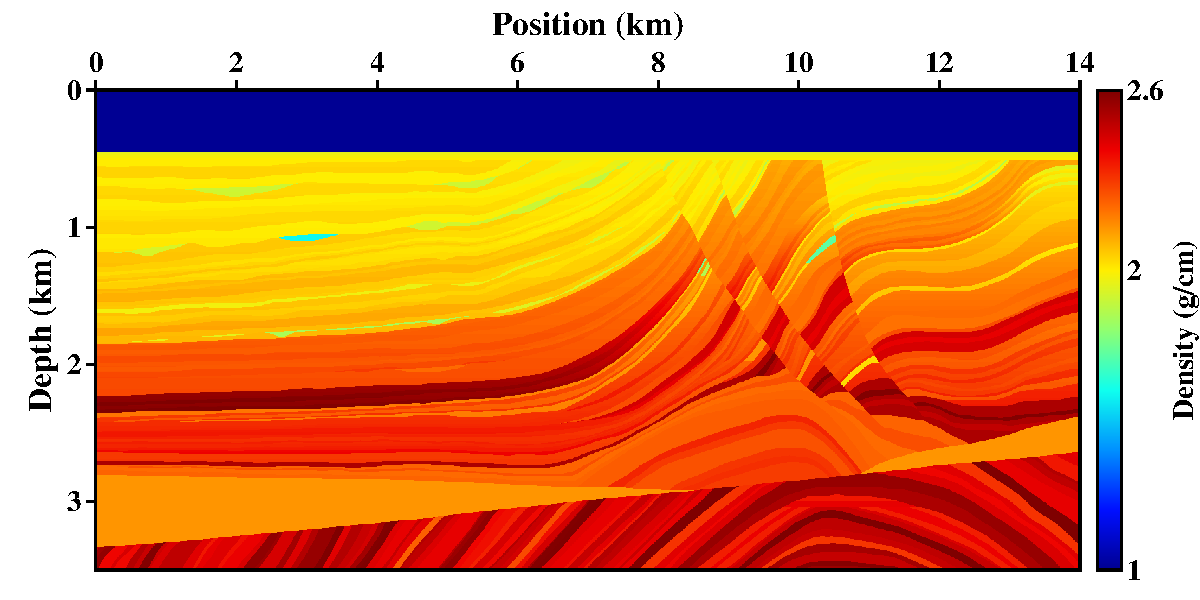
\includegraphics[width=7cm]{Figure/chapter02/tariqsugresult/Fig/truerho.pdf}}
        \subfloat[]{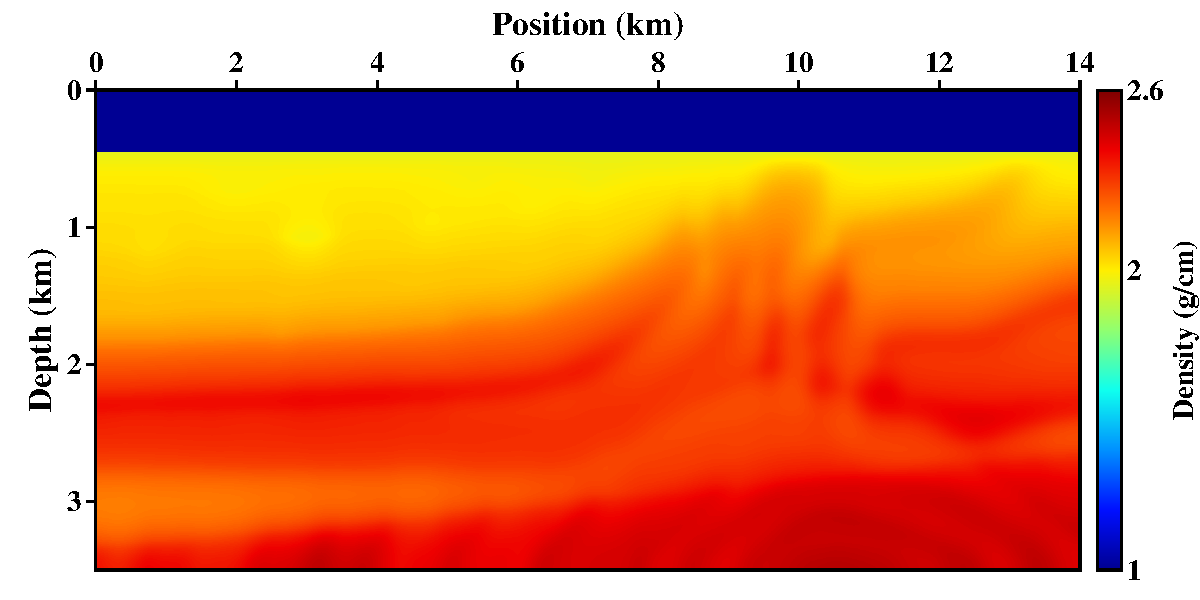
\includegraphics[width=7cm]{Figure/chapter02/tariqsugresult/Fig/initrho.pdf}}
    \caption{
		真实(a)和初始(b)Marmousi-II的密度模型
%                The true (a) and initial (b) density Marmousi-II model.
    }
    \label{fig:Marrho}
    \end{center}
\end{figure*}

采用速度-密度参数化方式,密度的梯度公式可以表示为\cite[]{mora:1987,kohn:2012}:
\begin{equation} 
    \hat{\mathbf{g}}_{\rho}=(V^2_p-2V^2_s)\mathbf{g}_{\lambda}+V^2_s\mathbf{g}_{\mu}+\mathbf{g}_{\rho},
    \label{eq:Gradient_rho} 
\end{equation}
其中$\mathbf{g}_{\lambda}$, $\mathbf{g}_{\mu}$和$\mathbf{g}_{\rho}$为采用$\rho$-$\lambda$-$\mu$参数化时的梯度,也即:
    \begin{equation} 
        \begin{split}
                \mathbf{g}_{\lambda}&=-\int_{0}^{T}\frac{\partial u_i}{\partial
        x_j}\frac{\partial \psi_k}{\partial x_l}
        \delta_{ij}\delta_{kl}dt,\\
                \mathbf{g}_{\mu}&=-\int_{0}^{T}\frac{\partial u_i}{\partial
        x_j}\frac{\partial \psi_k}{\partial x_l} 
        (\delta_{ik}\delta_{jl}+\delta_{il}\delta_{jk})dt,\\
                \mathbf{g}_{\rho}&=-\int_{0}^{T}\frac{\partial^2 u_i}{\partial
        t^2}\psi_idt.
        \end{split}
        \label{eq:DeGradient_vpvsrho}
    \end{equation}
如前文所述,在Born近似下,S波数据对$V_s$的扰动更敏感,基于以上事实前文采用了解耦梯度的方式来同时反演$V_p$和$V_s$。然而,考虑密度反演时,由于密度扰动
同时产生P与S波散射数据,因此上述逻辑就不再成立。联合方程\eqref{eq:DeGradient_vpvs}和\eqref{eq:Gradient_rho}来进行三参数同时反演。采用同样的
观测系统和反演策略并引入原始Marmousi密度模型来进行数值实验。

如图\ref{fig:InvertWithRho}所示,由于强烈的参数耦合效应,采用PCG优化的常规EFWI方法对三个参数都未能获得合理的重建。在模型左侧软海底区域,在引入密度变化后,
反演的病态性变得更强。$V_p$和$V_s$之间的耦合甚至导致反演结果中结构的错位。在采用MDPCG之后, $V_p$和$V_s$的反演都获得了很大的改善,但是密度的反演
结果仍然不准确,包含了较多来自$V_s$扰动的“脚印”(见图\ref{fig:RhoProfile3km}和图\ref{fig:RhoProfile9km})。不管如何,可以看到模式解耦可以降低反问题病态程度并提高反演模型的分辨率。若想进一步改善密度反演,
就需要用到更多的多尺度策略以及Hessian的逆来更好的压制参数耦合效应。
\begin{figure*}
    \begin{center}
        \subfloat[]{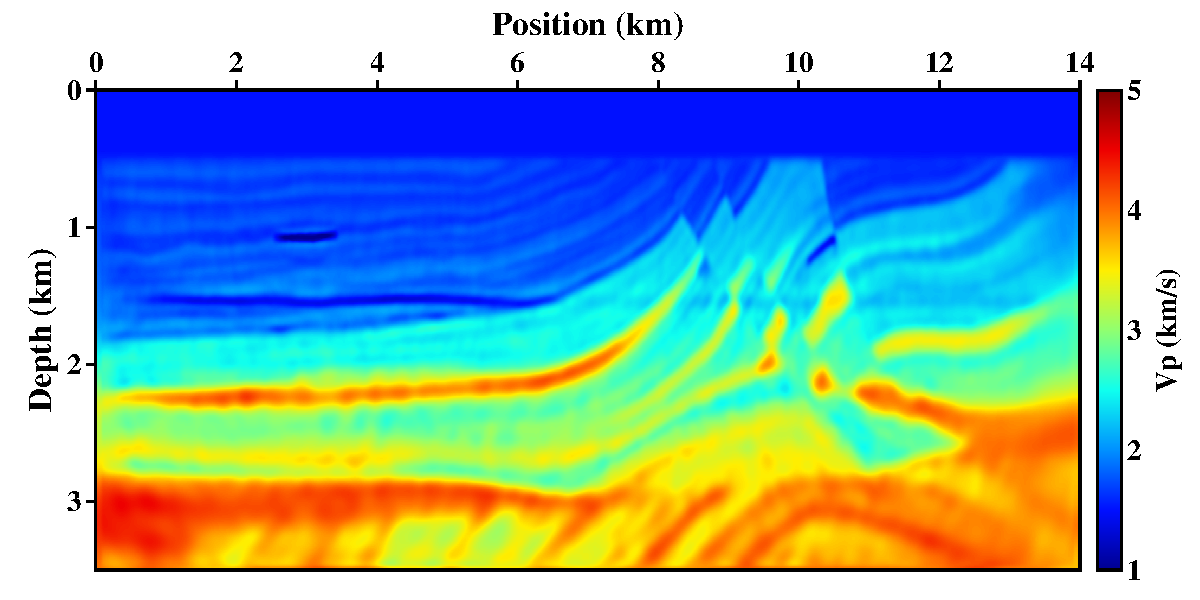
\includegraphics[width=7cm]{Figure/chapter02/tariqsugresult/Fig/1nodevp.pdf}}
        \subfloat[]{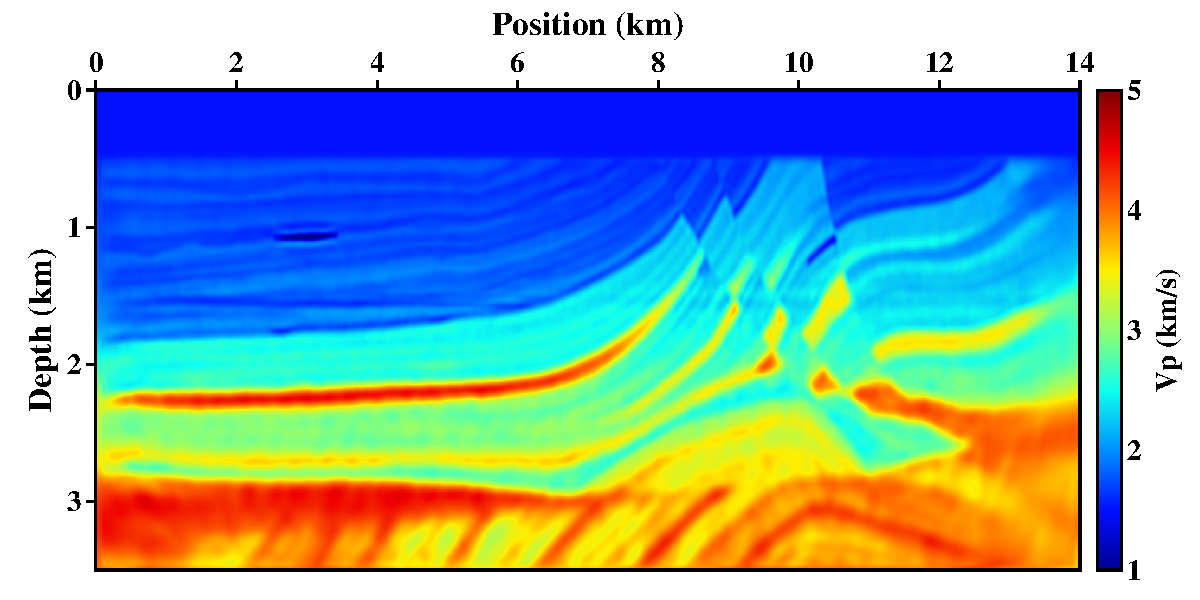
\includegraphics[width=7cm]{Figure/chapter02/tariqsugresult/Fig/1devp.pdf}}\\
        \subfloat[]{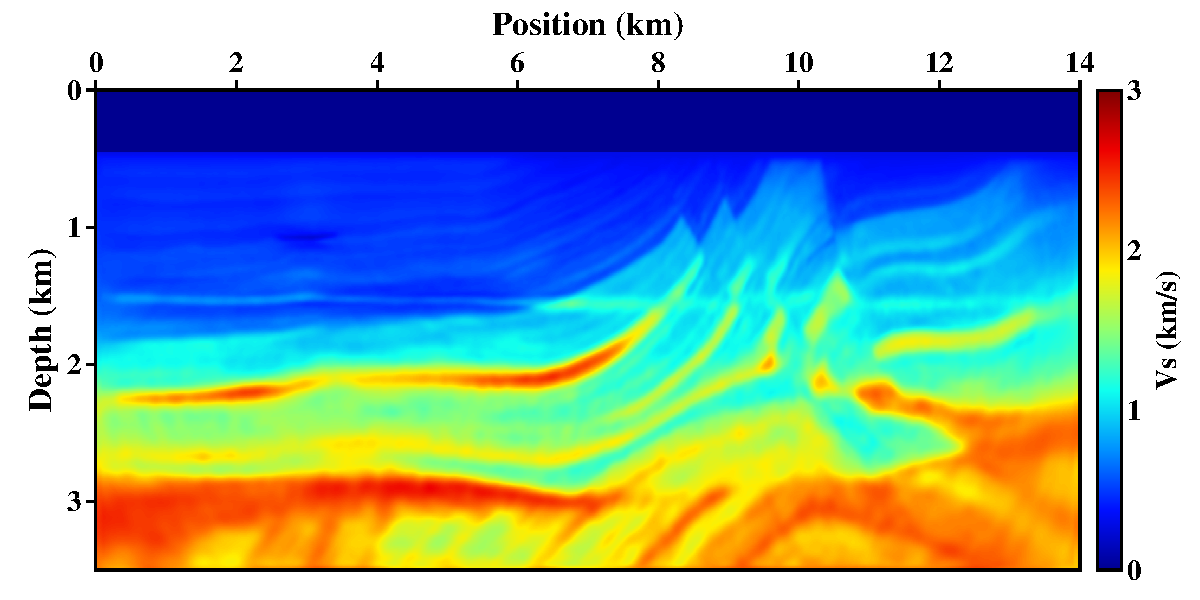
\includegraphics[width=7cm]{Figure/chapter02/tariqsugresult/Fig/1nodevs.pdf}}
        \subfloat[]{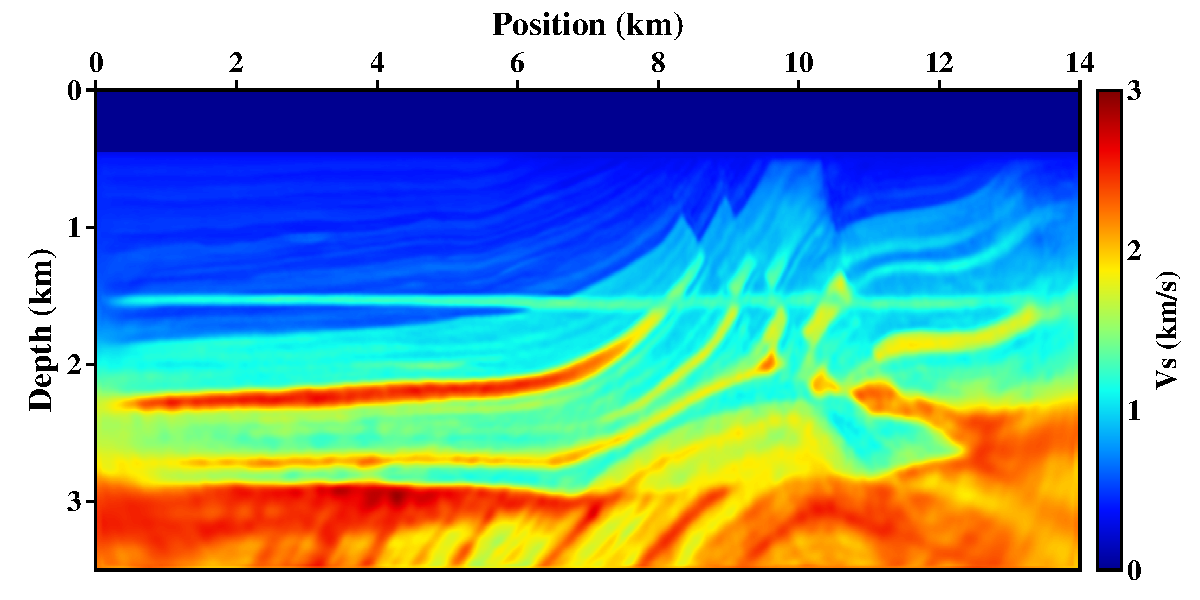
\includegraphics[width=7cm]{Figure/chapter02/tariqsugresult/Fig/1devs.pdf}}\\
        \subfloat[]{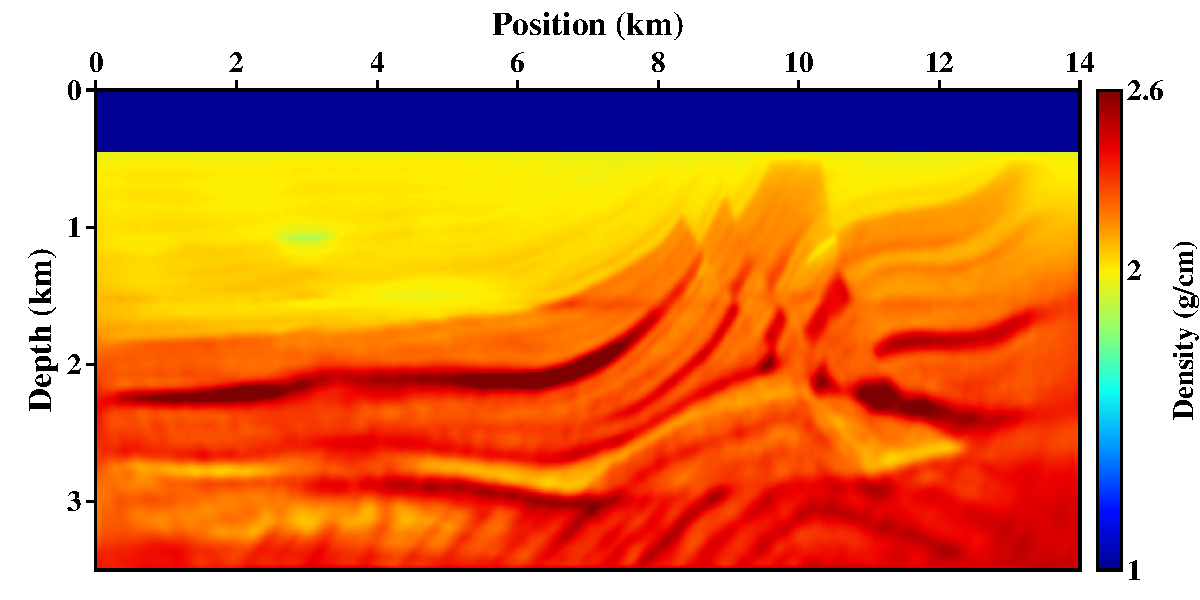
\includegraphics[width=7cm]{Figure/chapter02/tariqsugresult/Fig/1noderho.pdf}}
        \subfloat[]{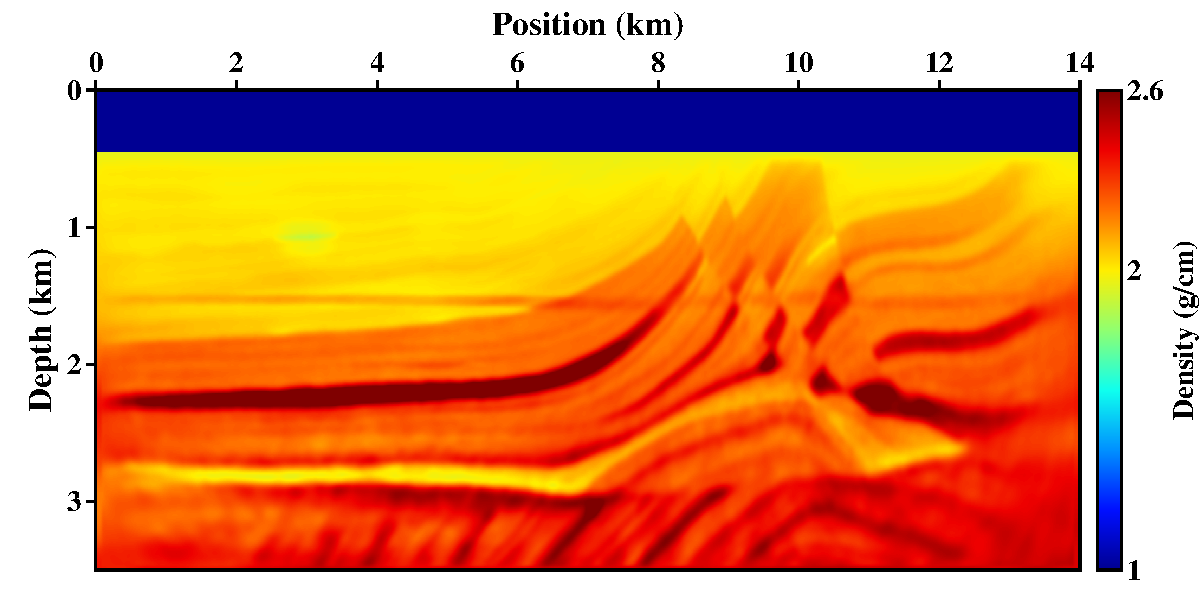
\includegraphics[width=7cm]{Figure/chapter02/tariqsugresult/Fig/1derho.pdf}}
        \caption{
			密度变化时常规和模式解耦的EFWI结果对比。左侧为常规PCG方法反演结果,右侧为MDPCG方法反演结果。
			其中(a),(b)为$V_p$; (c), (d)为$V_s$; (e), (f)为$\rho$。
%			Comparison between conventional and MD-based method with density
%            variation: (a) - (c) are the inverted $V_p$, $V_s$ and $\rho$ with
%            conventional method, (d) - (f) are the inverted $V_p$, $V_s$ and $\rho$
%            with MD-based method. 
		}
    \label{fig:InvertWithRho}
    \end{center}
\end{figure*} 

\section{本章小结}
多参数耦合效应使得常规梯度类EFWI受到很大挑战,即使在只考虑P和S波速度的反演时也是如此。辐射模式表明两种速度扰动都会产生P波数据扰动从而导致在特定散射角范围内的
重叠效应。相反,S波扰动波场则只与S波速度扰动相关。通过引入弹性波模式解耦,本文发现在解耦之后,不同波模式的Frech{$\acute{e}$}t和数据残差之间的互相关对梯度
的贡献非常微弱。通过该交叉项近似,导出了基于模式解耦的梯度,该梯度可以通过伴随状态法快速计算得到。利用解耦之后的Frech{$\acute{e}$}t导数,调查了
Hessian以及分辨率矩阵对应于P波与S波数据的有关分量。这些调查确认了在S波速度的梯度计算中丢弃P波分量可以降低参数耦合效应。因此,采用基于模式解耦的方法
来反演$V_s$等价于采用S波数据的单参数反演。借助较好的预条件算子消除S波数据的照明以及有限带宽效应,就能获得近似GN方法的收敛速度而不涉及
任何Hessian相关的计算。对于双参数同时反演,$V_s$反演的改善可以明显提高$V_p$的反演精度。数值实验尤其是包含软海底结构的Marmousi模型实验,表明模式解耦方法
对压制参数耦合、加速收敛是有效的。

到目前为止,通过波形反演来重建可靠的密度模型仍然非常困难。正如我们所看到的那样,模式解耦并未改善密度反演结果。但是在引入密度扰动后,反演病态性明显加剧后,采用MDPCG方法的EFWI仍能保证
获得比较合理的$V_p$和$V_s$结果。
\begin{figure}[!htb]
    \begin{center}
        {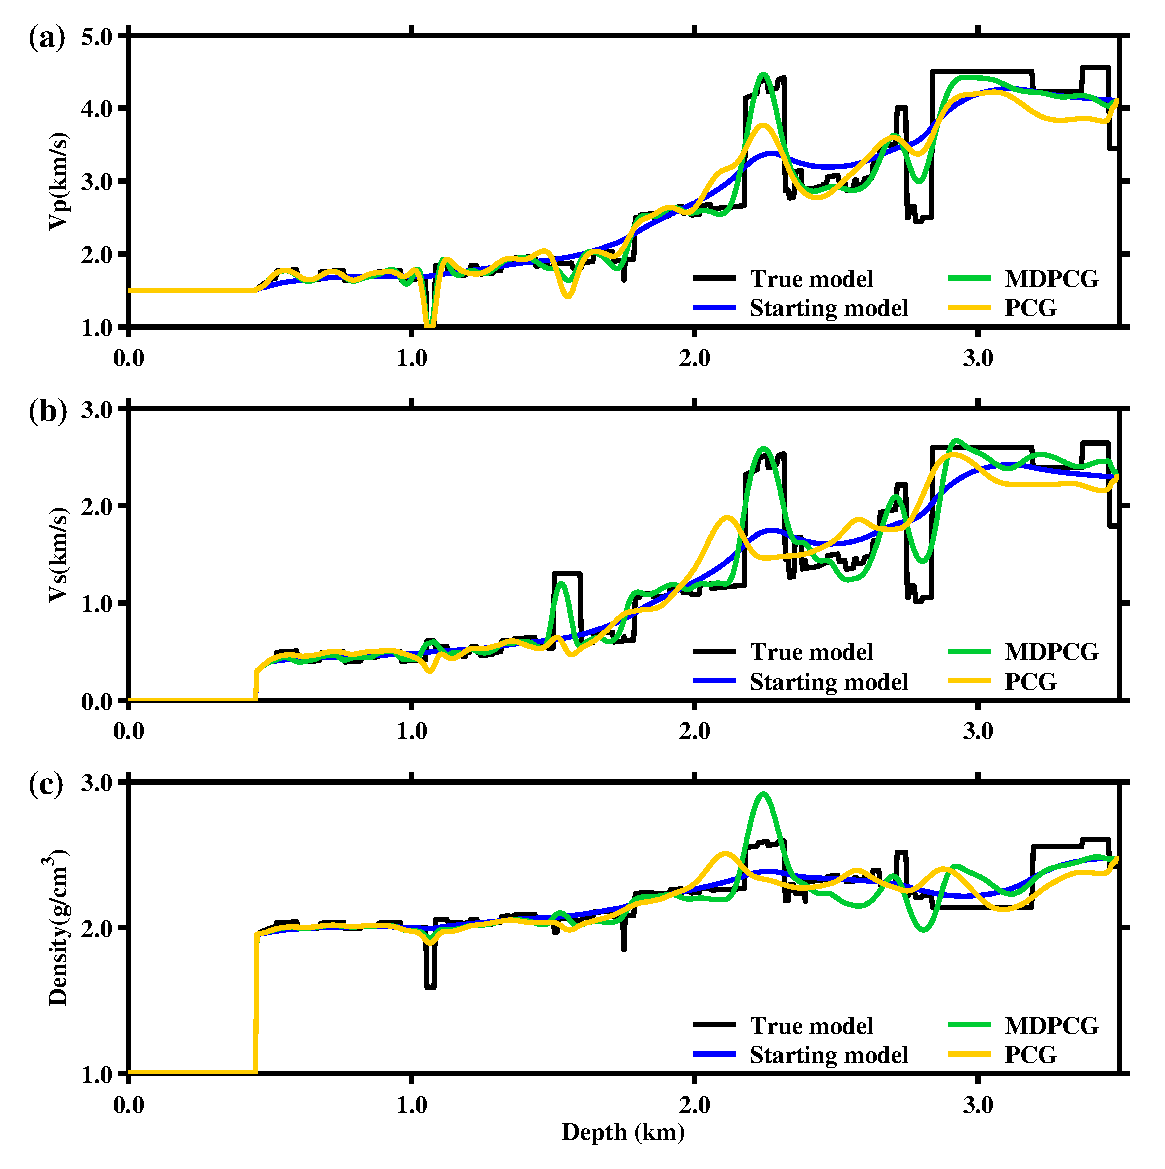
\includegraphics[width=10cm]{Figure/chapter02/tariqsugresult/Fig/3kmrho.pdf}}
        \caption{
			速度与密度模型在3.0km处的纵向剖面。
			黑线和蓝线分别代表真实和初始模型;黄线与绿线分别代表常规PCG和MDPCG方法反演结果。
%        The velocity and density profiles at 3.0 km (a, b)  with the true models
%            (black),
%            the initial models (blue), the PCG-based (yellow) and MD-based (green)
%            inverted models.
    }
    \label{fig:RhoProfile3km}
    \end{center}
\end{figure}
\begin{figure}[!htb]
    \begin{center}
        {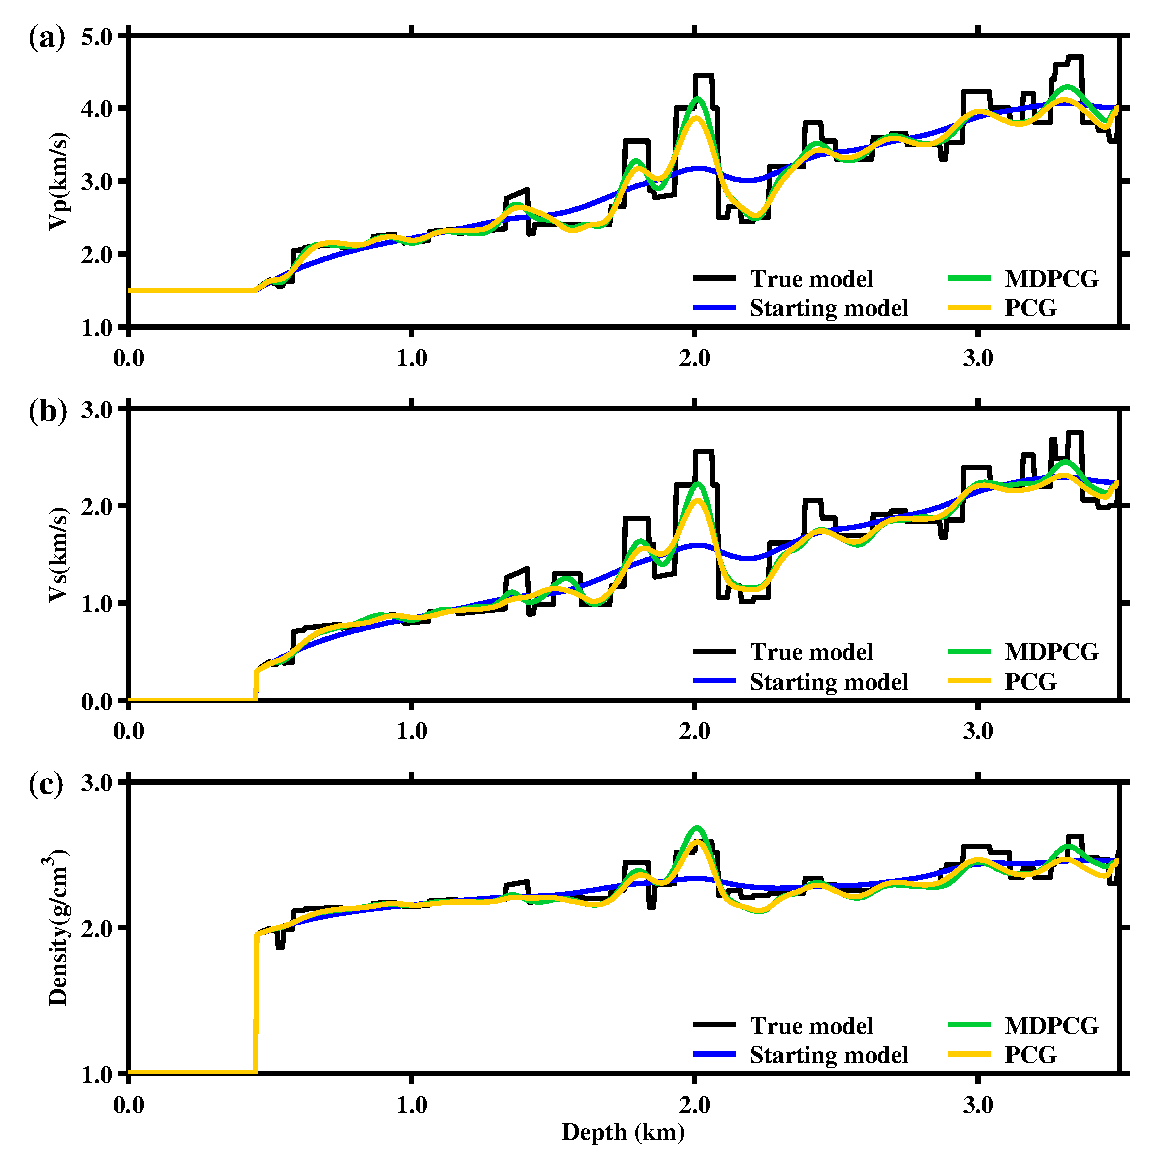
\includegraphics[width=10cm]{Figure/chapter02/tariqsugresult/Fig/9kmrho.pdf}}
        \caption{
			速度与密度模型在9.0km处的纵向剖面。
			黑线和蓝线分别代表真实和初始模型;黄线与绿线分别代表常规PCG和MDPCG方法反演结果。
%        The velocity and density profiles at 9.0 km (a, b)  with the true models
%            (black),
%            the initial models (blue), the PCG-based (yellow) and MD-based (green)
%            inverted models.
    }
    \label{fig:RhoProfile9km}
    \end{center}
\end{figure} 

%\chapter{弹性波波动方程反射走时反演}

\section{引言}
%尽管常规FWI在长偏移距,宽方位数据中有着令人满意的效果,但是在这种观测系统下,
目前FWI应用成功的案例中,主要利用了长偏移距透射波以及临界反射波等来更新速度模型的
中低波数分量。中深部的模型更新则主要集中在偏移响应对应的高波数部分。
在中深部区域,即使以目前大偏移距、宽方位的观测技术也难以保证有足够的透射波穿过。
如何利用现有数据准确反演中深部速度模型的中低波数成分是人们非常关心的课题。

反射波可以更好地照明深部结构。
受MBTT方法的启发,Xu et al
(2012)\cite{xu:2012}提出了反射波波形反演方法(RWI),
通过反射波来产生类似透射路径的信息来获得中低波数成分的更新。
RWI基于波动理论建立中深部背景模型的思路立即获得了广泛的关注(Wang et al., 2013\cite{Wang2013}; Wu and Alkhalifah, 2015; 
Zhou et al., 2015\cite{zhou:2015}; Guo and Alkhalifah, 2016\cite{Guo2016})。
它实质是通过最小平方偏移等手段获取“真振幅”的反射率,然后利用反偏移预测出反射波数据,并将它与观测数据的波形残差
反投影到Born波路径上进行背景速度更新。
%近期,Irabor and
%Warner(2016)\cite{Irabor2016}和Wang et
%al(2016)\cite{WangFangEtAl2016}在初始模型中加入高频扰动并通过上下形波分离来获取常规FWI中能够更新背景速度的梯度分量,实质上也利用了反射波波路径的信息。
%然而波形匹配并非是RWI中最合适的拟合方式。
尽管RWI的目的在于更新背景速度,
当初始模型偏离真值较远时,反射波波形匹配也会受到cycle-skipping影响。这时分频等多尺度策略会有助于避免cycle-skipping现象\cite{Wang2013}。此外,利用
走时信息构建目标函数也可以较好地避免上述问题。

在成像域利用反射波更新背景速度的方法由来已久,如射线层析\cite{Stork1992}。波动方程速度偏移分析(WEMVA)近年来也获得了长足的发展(
Sava and
Fomel(2006)\cite{SavaEtAl2006}; Yang and Sava(2011)\cite{YangEtAl2011}; Almomin and
Biondi(2012)\cite{Almomin2012}; Sun and Symes(2012)\cite{SunEtAl2012})。
WEMVA通常需要引入扩展成像条件,采用各类准则衡量成像残差,例如叠加能量最大(SI)\cite{ChaventEtAl1995}、微分相似优化(DSO)\cite{SymesEtAl1991}
和差异剩余偏移(DRM)\cite{SavaEtAl2004}等来实现背景模型的更新。
但WEMVA受困于昂贵的计算代价,尤其在三维问题中。
%针对反射走时,Luo et
%al(2016)\cite{Luo2016}用时间轴方向的扩展成像与Rytov近似结合,导出了全走时反演(FTI)方法,获得了不错的反演效果。该方法实质上也是一种成像域的反演方法。

为了克服振幅拟合有关的目标函数带来的非线性,本章采用与背景速度更加线性相关的
走时信息来构建目标函数。通过动态图像识别(DIW)技术来获取模拟与观测反射数据之间的时移量\cite{ma2013},提出了弹性波波动方程反射走时反演(EWERTI)方法。
相比互相关提取时移(空移)量的方式\cite{chi2015,Wang2015},DIW能更准确地获取局部的走时差异。
%Ma and
%Hale(2013)\cite{ma2013}采用动态图像识别(DIW)来获得模拟与观测反射数据之间的时移,从而导出了波动方程反射走时反演(WERTI)。Chi
%et al (2015)\cite{chi2015}和Wang et al
%(2015)\cite{Wang2015}采用互相关类的方法来获取时移(或空移)。
此外,弹性波走时反演中需要处理模式转换产生的虚假反射波路径的问题,即
需要根据对应的PP波与PS波波路径(假设P波震源)更新$V_p$与$V_s$模型。
文中将联合地面P/S分离+DIW获取不同波模式的走时残差,并通过空间波场模式解耦预条件梯度来降低非线性程度、压制参数耦合等。
在此基础上,设计出两步的反演流程来实现稳健的EWERTI方法。Sigsbee2A模型的数值实验将验证EWERTI方法的有效性。
%但尽管如此,RWI中的强非线性问题仍然存在,尤其是在使用波形匹配的目标函数时。
%虽然波形信息能提高反演精度,但是走时信息对模型的低波数成分扰动更敏感,二者之间具有更好的线性关系。
%因此我们使用走时残差的$L_2$范数
%作为目标函数,而走时信息则采用DIW获取。
%由于PP与PS走分别包含在在P波与S波地震记录中,因此还需要采用地面数据分离的方式
%分解出P或S波数据,才能保证准确获取PP和PS波走时信息。%本章中采用EWERTI的方式,通过两步法的策略建立$V_p$与$V_s$的背景模型。
%所以,采用走时反演来为常规FWI建立合适的含有长波长信息的初始
%%模型会更加稳健有效\cite[]{Ma2013, Chi2015, Luo2016}。然而在弹性介质中,这中思路会受到限制,
%因为弹性波场中存在复杂的模式转换,这就导致很难获得单一波模式的走时
%信息。
\section{弹性波波动方程反射走时反演}
利用拟合反射波来反演模型参数就需要预测出反射波数据,再与观测数据进行匹配。
弹性反射波的模拟通常采用偏移/反偏移的方式实现。
在EWERTI中,需要匹配反射波数据的走时信息,
并将走时残差反投影到反射波路径上更新背景速度模型。下面从弹性波方程出发导出EWERTI的梯度公式。
反演过程中,
同样假设在背景弹性介质($c_{ijkl}$)中有参数扰动$\delta c_{ijkl}$,则背景波场与扰动波场分别满足以下方程:
\begin{equation}
    \rho \frac{\partial u^2_i}{\partial t^2}  -
    \frac{\partial}{\partial x_j}\left[ 
        c_{ijkl}\frac{\partial u_{k}}{\partial
        x_l}\right]=f_i,
    \label{eq:WE_3} 
\end{equation}
和
\begin{equation}
    \rho \frac{\partial \delta u^2_i}{\partial t^2}  -
    \frac{\partial}{\partial x_j}\left[ 
        c_{ijkl}\frac{\partial \delta u_{k}}{\partial
        x_l}\right]=\frac{\partial}{\partial x_j}\left[\delta c_{ijkl}\frac{\partial u_{k}}{\partial x_l}\right],
    \label{eq:DeltaWE} 
\end{equation}
这里$\delta u_i$可以看作是用ERTM或其他方法获得的成像结果($\delta c_{ijkl}$)进行反偏移构建的反射波数据。
观测数据$\mathbf{d}^{o}$与模拟数据$\mathbf{d}^{c}$之间的走时残差需要达到最小,则目标函数写成:
\begin{equation}
	\left\{
		\begin{aligned}
			&\tau(\mathbf{x_r},t;\mathbf{x_s})=\mathop{\arg\min}_{\tau}
			\parallel\mathbf{d}^{c}(\mathbf{x}_r,t;\mathbf{x}_s)-\mathbf{d}^{o}(\mathbf{x}_r,t+\tau;\mathbf{x}_s)\parallel^2\\
    &E=\frac{1}{2}\int\tau^2(\mathbf{x_r},t;\mathbf{x_s})dtd\mathbf{x_r}d\mathbf{x_s},
		\end{aligned}
	\right.
    \label{eq:Objectivefunction} 
\end{equation}
其中走时残差$\tau(\mathbf{x_r},t;\mathbf{x_s})$可以通过DIW技术来获取。通过类似Ma and
Hale (2013)\cite{ma2013}的推导(见附录\ref{cha:AdjointForEWERTI}),本文导出了如下梯度公式:
\begin{equation}
    \frac{\partial E}{\partial c_{ijkl}}=-\int (\frac{\partial u_{i}}{\partial
    x_j}\frac{\partial \delta \psi_{k}}{\partial x_l}+\frac{\partial \delta u_{i}}{\partial
    x_j}\frac{\partial \psi_{k}}{\partial x_l}),
    \label{eq:GradientCijkl}
\end{equation}
其中,$\psi_i$和$\delta \psi_i$是共轭的背景波场和散射波场,满足:
\begin{equation}
    \rho \frac{\partial \psi^2_i}{\partial t^2}  -
    \frac{\partial}{\partial x_j}\left[ 
        c_{ijkl}\frac{\partial \psi_{k}}{\partial
        x_l}\right]=\tau(\mathbf{x_r},t;\mathbf{x_s})\frac{\dot{d}^o_i(\mathbf{x_r},t+\tau;\mathbf{x_s})}{h_i(\mathbf{x_r},t;\mathbf{x_s})},
    \label{eq:AdjointWE} 
\end{equation}
和
\begin{equation}
    \rho \frac{\partial \delta \psi^2_i}{\partial t^2}  -
    \frac{\partial}{\partial x_j}\left[ 
        c_{ijkl}\frac{\partial \delta \psi_{k}}{\partial 
        x_l}\right]=\frac{\partial}{\partial x_j}\left[\delta c_{ijkl}\frac{\partial
        \psi_{k}}{\partial x_l}\right], 
    \label{eq:AdjointDeltaWE} 
\end{equation}
式中$h_i(\mathbf{x_r},t;\mathbf{x_s})=(\dot{d}^o_i(\mathbf{x_r},t+\tau;\mathbf{x_s}))^2-\ddot{d}^o_i(\mathbf{x_r},t+\tau;\mathbf{x_s})
(d^c_i(\mathbf{x_r},t;\mathbf{x_s})-d^o_i(\mathbf{x_r},t+\tau;\mathbf{x_s}))$,而$\dot{d}$则代表$d$的时间导数。
需要注意的是,上式伴随源的分母中包含有地震记录的二阶导数,会导致除法的不稳定,这里采用时间方向的积分
$h^{'}_i(\mathbf{x_r};\mathbf{x_s})=\int h_i(\mathbf{x_r},t;\mathbf{x_s})dt$
来代替原有的分母项(付继有等,2015\cite{Fu2015})。
在方程\eqref{eq:GradientCijkl}的右端
,第一和第二项分别表示震源端和检波点端的反射波路径。可以通过链式法则导出P波与S波速度的梯度公式:
\begin{equation}
\begin{split}
    &\frac{\partial E}{\partial V_p}=2\rho V_p\frac{\partial E}{\partial
        c_{ijkl}}\delta_{ij}\delta_{kl}, \\
    &\frac{\partial E}{\partial V_s}=2\rho V_s\frac{\partial
    E}{\partial c_{ijkl}}(-2\delta_{ij}\delta_{kl}+\delta_{ik}\delta_{jl}+
    \delta_{il}\delta_{jk}).
\end{split}
    \label{eq:GradientVel}
\end{equation}

\section{弹性波反射波路径核函数}
反射波反演的关键是将预测的与观测的反射波之间的残差反投影到反射波路径上,从而实现对模型的更新。因此,反射波波路径的计算将是反演中
的核心任务。由于弹性波中存在各种模式转换,所以反射波波路径的复杂程度远大于声波中的情况。首先分析弹性波反射波路径的性态,并尝试通过
模式解耦克服反演中遇到的部分困难。
由附录\ref{cha:AdjointForEWERTI}推导可看出,不同的目标函数只影响共轭状态方程的伴随震源项,并不影响最终梯度的互相关方式。
因此分析弹性反射波波路径的核函数性态将有助于理解模式耦合引起的问题,从而为压制梯度中的假象并帮助设计新的反演策略提供理论依据。
\begin{figure}[!htb]
   \centering
   \subfloat[]{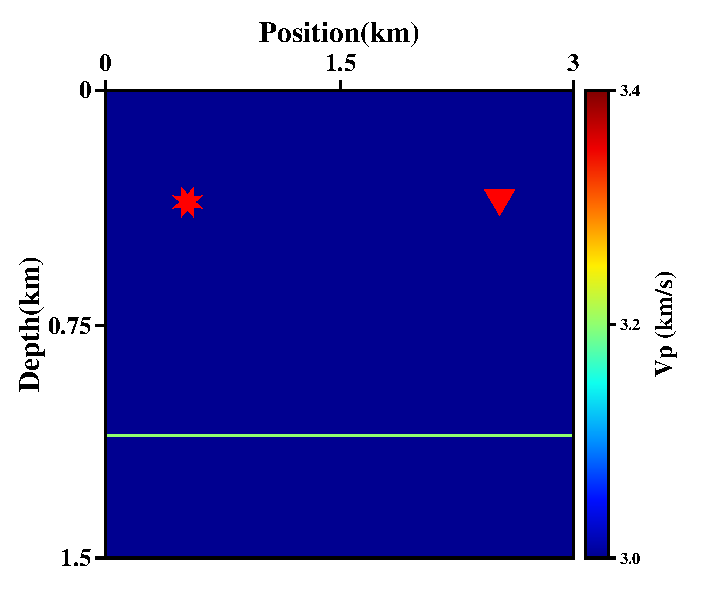
\includegraphics[width=0.50\textwidth]{Figure/chapter03/Kernel/1vp.pdf}}
   \subfloat[]{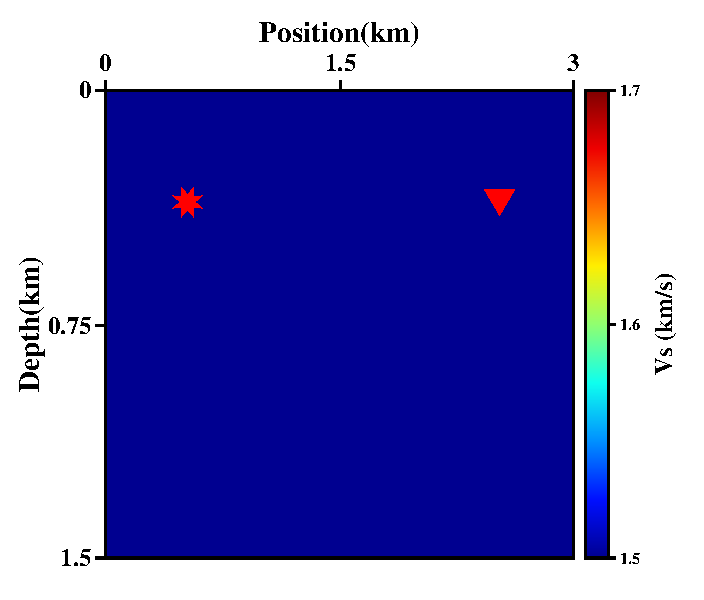
\includegraphics[width=0.50\textwidth]{Figure/chapter03/Kernel/1vs.pdf}}\\
   \subfloat[]{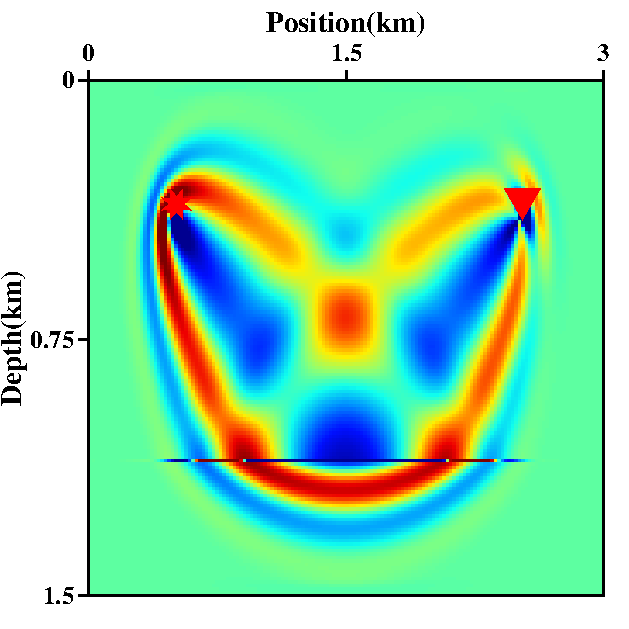
\includegraphics[width=0.50\textwidth]{Figure/chapter03/Kernel/Vponlyvp.pdf}}
   \subfloat[]{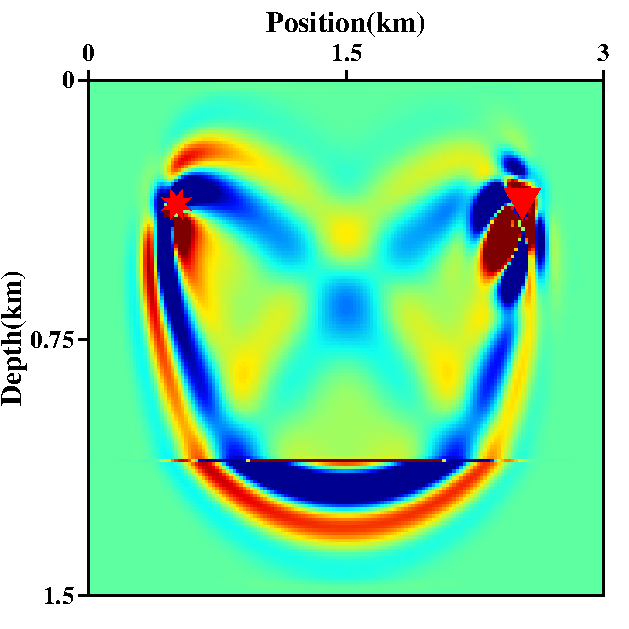
\includegraphics[width=0.50\textwidth]{Figure/chapter03/Kernel/Vsonlyvp.pdf}}\\
   \caption{单$V_p$界面的反射波路径。(a) $V_p$模型,(b) $V_s$模型,(c) $V_p$敏感核函数,(d) 
   $V_s$敏感核函数.}
   \label{fig:kernel1_vp}
\end{figure}

为了简化表达,将式\eqref{eq:GradientCijkl}重新写作:
\begin{equation}
    \nabla E(
    \mathbf{m}_0)=-\int(
    \mathbf{u}\cdot\delta \boldsymbol{\psi}
    +\delta
    \mathbf{u}\cdot{\boldsymbol{\psi}})
    \label{eq:kernelgradient} 
\end{equation} 
其中$\mathbf{u}$和$\boldsymbol{\psi}$为背景介质的正传与共轭波场,$\delta\mathbf{u}$和$\delta \boldsymbol{\psi}$为正传与共轭的散射场。
这里统一用$\cdot$表示波场分量的互相关。上式只示意性表达出反射波路径的计算方式,而不同参数化方式相应的具体计算公式需要参照链式法则获得。
上式中第一项表示震源到反射界面的波路径,第二项表示从反射界面到检波点的波路径。考虑到
波场解耦,上式的梯度也可以分解成P或S波数据组合的分量:
\begin{equation}
    K_m^{MN}     
    =-\int(\mathbf{u}^M\cdot\delta \boldsymbol{\psi}^N
    +\delta  \mathbf{u}^M\cdot\boldsymbol{\psi}^N),\\
    \label{eq:decompkernel} 
\end{equation}
其中$m\in\{V_p, V_s\}$,$M,N\in\{P,S\}$。

为了观察弹性波反射波路径(敏感核函数),先在单界面模型中计算反射波波路径。假定只有$V_p$的扰动界面(如图\ref{fig:kernel1_vp}a和b)。
%\begin{figure}
%   \centering
%   \subfloat[]{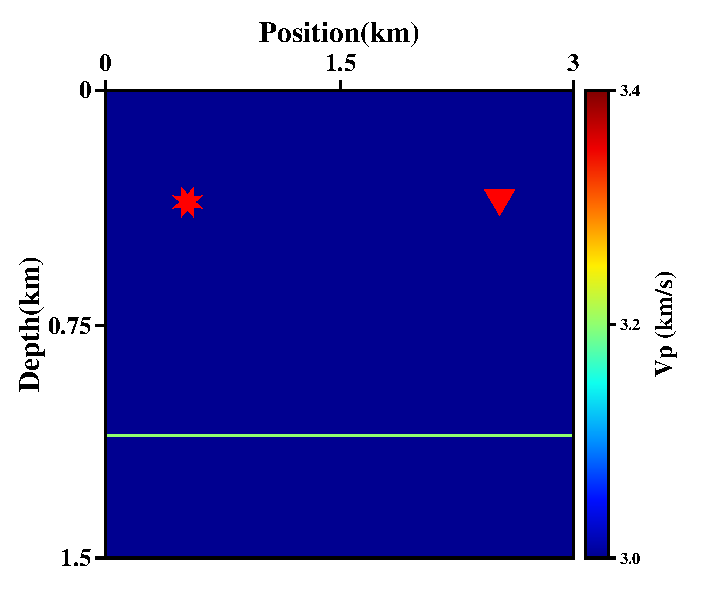
\includegraphics[width=0.38\textwidth]{Figure/chapter03/Kernel/1vp.pdf}}
%   \subfloat[]{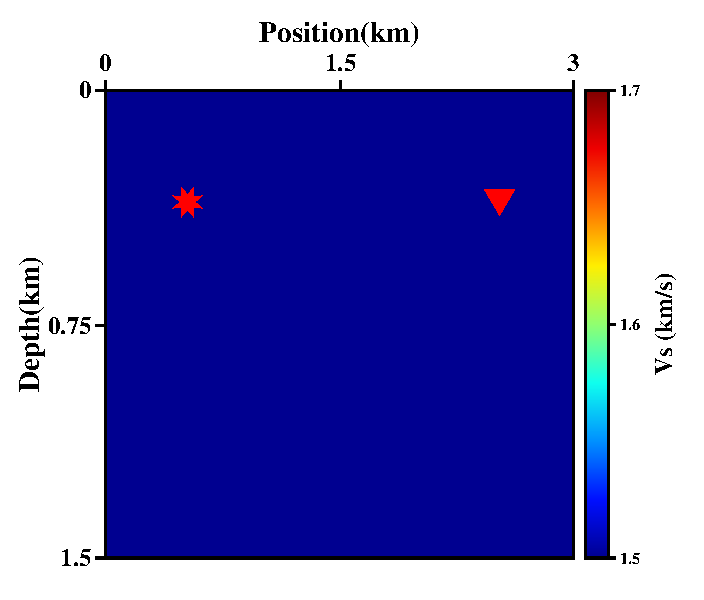
\includegraphics[width=0.38\textwidth]{Figure/chapter03/Kernel/1vs.pdf}}\\
%   \caption{单独$V_p$扰动界面。左侧为$V_p$,右侧为$V_s$.}
%   \label{fig:KernelModel1}
%\end{figure}
由于没有$V_s$扰动,因此没有模式转换能量而只有PP波反射,非常接近于声波情况。
采用该模型获得的反射波波路径如图\ref{fig:kernel1_vp}c和d。可以看到,$V_p$的反射波
路径分为震源端以及检波点端左右两支,与声波波路径非常接近。同时,$V_s$也会有相应的波路径能量,但是主要集中在边缘部分,第一菲涅尔带中央区域
能量较弱。原因可能是这部分波路径信息是与PP波反射能量对应的,对$V_s$背景信息并不敏感。
%如果换做$\lambda$和$\mu$的参数化方式,其产生的波路径如图\ref{Kernel1_lambda}所示
%\begin{figure}
%   \centering
%   \subfloat[]{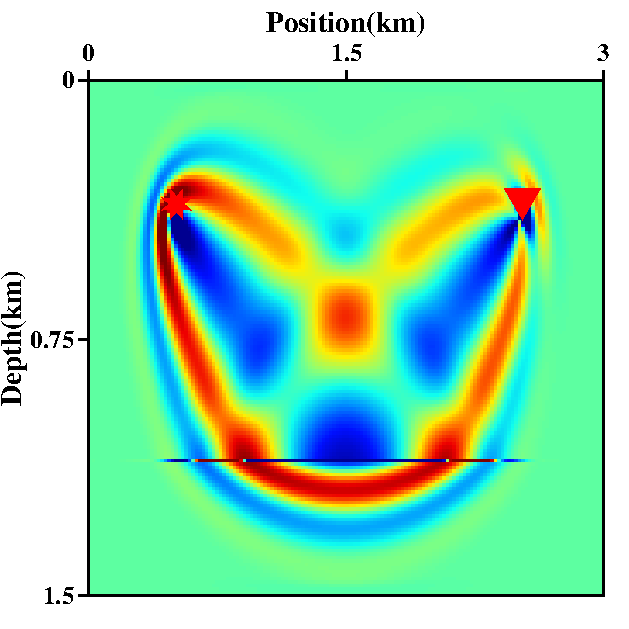
\includegraphics[width=0.30\textwidth]{Figure/chapter03/Kernel/lambdaonlyvp.pdf}}
%   \subfloat[]{\includegraphics[width=0.30\textwidth]{Figure/chapter03/Kernel/muonlyvp.pdf}}\\
%   \caption{图\ref{fig:KernelModel1}模型$\lambda$参数化时的反射波路径。左侧为$\lambda$,右侧为$\mu$.}
%   \label{fig:kernel1_lambda}
%\end{figure}
\begin{figure}[!htb]
   \centering
   \subfloat[]{\includegraphics[width=0.50\textwidth]{Figure/chapter03/Kernel/2vp.pdf}}
   \subfloat[]{\includegraphics[width=0.50\textwidth]{Figure/chapter03/Kernel/2vs.pdf}}\\
   \subfloat[]{\includegraphics[width=0.50\textwidth]{Figure/chapter03/Kernel/Vponlyvs.pdf}}
   \subfloat[]{\includegraphics[width=0.50\textwidth]{Figure/chapter03/Kernel/Vsonlyvs.pdf}}\\
   \caption{单$V_s$界面的反射波路径。(a) $V_p$模型,(b) $V_s$模型,(c) $V_p$敏感核函数,(d) 
   $V_s$敏感核函数.}
%   \caption{单独$V_p$扰动界面。左侧为$V_p$,右侧为$V_s$.}
   \label{fig:kernel2}
\end{figure}

然后,考虑$V_s$模型存在界面的情况(图\ref{fig:kernel2}a和b)。此时波场就会变得十分复杂
,在正传及反传波场中会同时存在P波与S波,导致反射波路径变得更加复杂。
%\begin{figure}
%   \centering
%   \subfloat[]{\includegraphics[width=0.30\textwidth]{Figure/chapter03/Kernel/Vponlyvs.pdf}}
%   \subfloat[]{\includegraphics[width=0.30\textwidth]{Figure/chapter03/Kernel/Vsonlyvs.pdf}}\\
%   \caption{单独$V_p$扰动时的反射波路径。左侧为$V_p$,右侧为$V_s$.}
%   \label{fig:kernel2}
%\end{figure}
\begin{figure}[!bth]
   \centering
   \subfloat[]{\includegraphics[width=0.50\textwidth]{Figure/chapter03/Kernel/VsonlyvsPP.pdf}}
   \subfloat[]{\includegraphics[width=0.50\textwidth]{Figure/chapter03/Kernel/VsonlyvsPS.pdf}}\\
   \subfloat[]{\includegraphics[width=0.50\textwidth]{Figure/chapter03/Kernel/VsonlyvsSP.pdf}}
   \subfloat[]{\includegraphics[width=0.50\textwidth]{Figure/chapter03/Kernel/VsonlyvsSS.pdf}}
   \caption{$K_{V_s}$敏感核函数的四个分量:(a) $K_{V_s}^{PP}$, (b) $K_{V_s}^{PS}$, (c) $K_{V_s}^{SP}$, (d) $K_{V_s}^{SS}$.}
   \label{fig:kernel2_vs_decomp}
\end{figure}
图\ref{fig:kernel2}中$V_p$敏感核函数与图\ref{fig:kernel1_vp}有所不同,这是因为当存在$V_s$反射界面时,反传的散射波场在界面处产生“非物理”的SP转换波,
这部分波场与背景场中的P波互相关就会产生一些假象。而在$V_s$的敏感核函数中,可以看到多种模式转换导致的多个波路径叠加,使得核函数十分复杂。
但是可以观察到其中的P波路径的能量总是占主导地位。
如果直接采用该核函数来计算目标函数关于$V_s$的梯度,一定会因为这些严重的cross-talk对反演带来更多的麻烦。

根据公式\eqref{eq:decompkernel},将原始的$V_s$核函数分解为四个部分。
如图\ref{fig:kernel2_vs_decomp}所示,$K_{V_s}^{PP}$与图\ref{fig:kernel2}c中
的$V_p$核函数十分类似,但是主要能量的符号相反(在第二章图\ref{fig:all}中有类似现象);$K_{V_s}^{PS}$与$K_{V_s}^{SP}$则包含非常多的高频信息,
它们主要是不同模式的正传与反传波场之间的偏移脉冲响应,如果不对这些高波数成分进行压制处理就会对$V_s$梯度的计算带来较多的高频干扰,不利于低波数背景速度的更新
;$K_{V_s}^{SS}$则与其他三者有些不同,只包含了检波点端的单支反射路径,这是由于
采用了P波震源,在震源端的波场中不包含S波数据($K_{V_s}^{SS}$的震源端项会是0)。这样的话,$K_{V_s}^{SS}$就几乎不受到P波路径的影响,且较少包含高波数的偏移响应。
如果利用好这些分解后核函数分量的特征,
将会非常有助于背景$V_s$的反演。

$\quad$

$\quad$
\section{反射走时反演流程}
弹性介质中P波震源情况下,不同模式的转换波(主要是PP与PS波)同相轴之间会互相叠加、互相交叉。在用DIW提取走时残差的时候,这些交叉点的位置就会变成一些奇异点带来很大麻烦
。因此,如果直接用原始多分量数据的话,拾取到的$\tau(\mathbf{x_r},t;\mathbf{x_s})$就会不准确,这也是为什么式\eqref{eq:AdjointDeltaWE}中的梯度很难直接应用。
为了解决这个问题,本文将观测与模拟地震数据分解为P波与S波两部分。该模式分解只作用于地面地震数据\cite[]{Li2016a},可以快速地获得每一炮数据分解之后的矢量
P波或S波地震记录。这样,走时残差就可以被分成P波与S波两部分,使得弹性波WERTI变得可行。于是,设计出一个两阶段的反演流程,先P波阶段后S波阶段。
由于DIW提取走时的方式对数据的频率成分并不敏感,因此EWERTI中的多尺度策略主要体现在参数反演先后顺序上,并不需要过多考虑分频的策略。
\subsection{$V_p$反演}
在这个阶段主要采用PP反射波来建立P波速度的背景模型。首先,从ERTM中获得P波速度的扰动,即$\delta V_p$。
因为在速度不准的情况下大偏移距数据的偏移/反偏移结果会
造成模拟的反射波零偏移距走时误差,进而增加反演的非线性程度。
这里为了确保模拟数据与观测数据中零(小)偏移距反射走时相匹配,只采用小偏移距的数据
获取$\delta V_p$。
此外,由于在EWERTI中只考虑走时,可以只进行ERTM成像
而不是ELSRTM来估计反射率。
这也降低了反演中对反射系数估计的依赖程度。因此,目标函数变为最小化PP反射波的走时残差:
\begin{equation}
    E_{pp}=\frac{1}{2}\int\tau^2_{pp}(\mathbf{x_r},t;\mathbf{x_s})dtd\mathbf{x_r}d\mathbf{x_s}.
    \label{eq:ObjectivefunctionPP} 
\end{equation}
这样,采用分离的P波记录来计算方程\eqref{eq:AdjointWE}的右端项,并用$\delta V_p$替换方程\eqref{eq:DeltaWE}和\eqref{eq:AdjointDeltaWE}中的$\delta c_{ijkl}$,
就可以计算得到$V_p$的梯度($\frac{\partial E}{\partial V_p}$)。与EFWI一样,该梯度中的互相关项自动隐含了散度算子。因此,在
计算时只利用了PP反射波,所以不需要额外施加空间域的模式解耦。这个PP波走时反演本质上接近于声波反射走时反演,区别在于需要将地
面多分量地震记录进行数据域模式分离。注意,在分离后的数据中可能包含部分SP模式的转换波,它们对$V_p$的反演可能造成不利的影响,这需要今后更深入的研究。

\subsection{$V_s$反演}
接下来将对PS反射波采用类似的反演。相应地,目标函数变为:
\begin{equation}
    E_{ps}=\frac{1}{2}\int\tau^2_{ps}(\mathbf{x_r},t;\mathbf{x_s})dtd\mathbf{x_r}d\mathbf{x_s}.
    \label{eq:ObjectivefunctionPS} 
\end{equation}
值得一提的是,PS反射波的模拟(预测)方式与前一阶段略有不同。这里有两种方式来模拟PS反射波:

方式\uppercase\expandafter{\romannumeral1}: 采用反演好的$V_p$以及初始$V_s$模型来实现PS波偏移成像,然后使用该成像结果进行反偏移;

方式\uppercase\expandafter{\romannumeral2}: 由于$V_p$的背景速度在前一阶段已经被较好地恢复,此时PP波成像结果应该比较接近准确位置。考虑到大多数情况下,地
下介质中$V_p$与$V_s$的界面是比较一致的,因此也可以采用PP波成像结果作为界面来模拟PS反射波。

经过测试,发现第一种方式产生的近偏移距走时
对$V_p$模型的误差非常敏感,即使$V_p$模型在真值附近扰动也有可能获得方向错误的走时残差。
对于非对称的PS反射波的路径,假定地下存在如图\ref{fig:PS_refl}所示的单界面PS波反射。
由几何关系以及Snell定律,存在如下关系
%入射角$\theta_1$与反射角$\theta_2$之间以及深度、偏移距与该角度之间的关系为:
\begin{equation}
%\begin{split}
    \frac{sin\theta_1}{V_p}=\frac{sin\theta_2}{V_s},\qquad
    h(tan\theta_1+tan\theta_2)=X,
%\end{split}
    \label{eq:Snell_PS} 
\end{equation}
\begin{figure}
   \centering
   \subfloat{\includegraphics[width=0.40\textwidth]{Figure/chapter03/PS_problem/PS_refl.pdf}}
   \caption{单界面PS反射波示意图。}
   \label{fig:PS_refl}
\end{figure}
其中$\theta_1$和$\theta_2$分别为入射和反射角,$h$为界面深度,则PS波时距曲线关系为:
\begin{equation}
	t=\frac{h}{cos\theta_1V_p}+\frac{h}{cos\theta_2V_s}.
    \label{eq:TravelTime_PS} 
\end{equation}
方式\uppercase\expandafter{\romannumeral1}与方式\uppercase\expandafter{\romannumeral2}的差异在于速度不准时,确定界面深度的过程不同。
这里数值分析时使用零(小)偏移距的图偏移获得界面深度,然后带入到
式\eqref{eq:TravelTime_PS}中来近似获得错误速度下反偏移预测的反射数据时距关系。

方式\uppercase\expandafter{\romannumeral1}
中,在图偏移时零偏移距走时保持不变,则偏移后的深度位置满足:
\begin{equation}
	\frac{h_{1}}{V^{'}_p}+\frac{h_{1}}{V^{'}_s}=\frac{h}{V_p}+\frac{h}{V_s},
    \label{eq:Mapmigration_PS} 
\end{equation}
其中$V^{'}_p$和$V^{'}_s$为错误的偏移速度。可以求得图偏移的深度:
\begin{equation}
	{h_{1}}=\frac{V^{'}_s(V_p+V_s)}{V_s(V^{'}_p+V^{'}_s)}h.
    \label{eq:ZerooffMig_PS} 
\end{equation}
而采用方式\uppercase\expandafter{\romannumeral2}时,在$V_p$存在误差时图偏移求得界面的深度为:
\begin{equation}
	{h_{2}}=\frac{V^{'}_p}{V_p}h.
    \label{eq:ZerooffMig_PP} 
\end{equation}
通常情况下
$V_p>V_s$因此$\frac{V_p+V_s}{V^{'}_p+V^{'}_s}$中$V^{'}_p$的小偏差也会带来很大的影响,
因此PS波零(小)偏移距成像界面的深度会同时受到$V_p$与$V_s$速度误差的影响。
下文将使用式\eqref{eq:Snell_PS}-\eqref{eq:ZerooffMig_PP}测试反偏移重建的反射数据的时距关系对$V^{'}_p$和$h$的敏感性。

这里将以下几个参数固定为$V_p=2500m/s$, $V_s=1500m/s$, $V^{'}_s=1300m/s$, 而$V^{'}_p$选取$2450,
2500, 2550m/s$三个扰动值。
从图\ref{fig:Sens_vp}可以看到,采用方式\uppercase\expandafter{\romannumeral1}时获取的反射数据对$V_p$的误差非常敏感,
在$\pm50m/s$范围内就会引起反偏移数据的走时残差改变方向
。相反,如果采用方式\uppercase\expandafter{\romannumeral2},其走时残差方向都是正确的。
\begin{figure}[h]
   \centering
   \subfloat[]{\includegraphics[width=0.5\textwidth]{Figure/chapter03/PS_problem/h1000.pdf}}
   \subfloat[]{\includegraphics[width=0.5\textwidth]{Figure/chapter03/PS_problem/h500.pdf}}
   \caption{不同界面深度时方式\uppercase\expandafter{\romannumeral1}(黑色虚线)与
   方式\uppercase\expandafter{\romannumeral2}(蓝色虚线)反偏移获得PS波走时曲线
   与真实值(红色实线)之间的对比。数字1,2,3分别代表不同$V^{'}_p$速度的结果。(a) 界面深度$h=1000$; (b) 界面深度$h=500$.}
   \label{fig:Sens_vp}
\end{figure}

所以,本文采用较为准确的PP成像($\delta V_p$)结果
%而不
%是$\delta V_s$
来产生PS反射波。
但这样做也存在两个弊端:
第一、产生的PS反射无法保证振幅的准确性,幸运的是这并不会给DIW拾取走时残差带来大的
困扰;第二、来自深部的PS反射可能由于时差太大使得DIW拾取受到cycle-skipping困扰。
不过这个问题可以采用“层剥离”的方式,通过照明能量补偿的控制,先使用浅部的反射走时残差来更新浅层,
再使用深部的走时残差更新深部的速度。这样即使初始阶段深部的反射走时残差拾取错误也不影响浅部的速度更新。
在浅部更新较好后,深部的反射走时残差也能保证拾取得较为准确。
%先更新浅层$V_s$
%然后更新深层来避免。
%但方式\uppercase\expandafter{\romannumeral2}也存在问题,
%即在界面深度较深时,Born模拟的走时偏离真值较远,如果存在多个同相轴就会难以进行震相间的匹配,这样即使DIW也会受到
%cycle-skipping影响,但幸运的是界面深度较浅时,Born模拟走时与观测数据偏离并不远,这样的话可以层剥离的方式来从浅到深反演
%解决深层反射的震相匹配问题。

此外,正如前文核函数分析提到,PS反射中震源端波路径只与P波速度相关,
因此在计算$\frac{\partial E}{\partial V_s}$时可以丢掉方程\eqref{eq:GradientCijkl} 
右端项的第一部分。同时,波模式分解也会施加在梯度的计算过程中来确保只有S波能量参与计算,即:
\begin{equation}
    \frac{\partial E_{ps}}{\partial V_s}=-2\rho V_s
    \int (\frac{\partial \delta u^S_{i}}{\partial
    x_j}\frac{\partial \psi^S_{k}}{\partial x_l})
    (\delta_{ik}\delta_{jl}+
    \delta_{il}\delta_{jk}).
    \label{eq:GradientVel_S}
\end{equation}
该模式解耦的梯度与Wang et al.
(2015)\cite{wang:2015}提出的EFWI预条件方式类似,可以在$V_s$的反演中降低参数耦合的影响

\section{局部倾角导引正则化}
数据域的WERTI与成像域射线走时层析有一些相似特性。通常,射线走时层析由于射线路径覆盖不均匀、反射界面深度与速度之间存在耦合等问题会导致反演的多解性,
所以射线层析通常不收敛或者很难收敛到正确的速度模型。
常规各向同性平滑算子的正则化约束可以一定程度上降低上述多解性的困扰,但是也很难保证反演收敛到具有地质含义的物理模型。
在偏移后,成像结果可以提供地下界面大致的倾角信息,由此设计正则化算子来沿地层倾角对反演进行约束可以
有效地应对多解性的问题,从而加快收敛速度、改善反演结果。由于采用波动方程作为波场传播引擎,WERTI采用波路径信息来反投影走时残差,因而所面临的多解性挑战要
小于射线走时层析。不过,对于一些照明不足或者
反射路径覆盖不均匀的区域同样也会产生多解性问题。因此,WERTI中采用局部倾角导引的正则化同样可以加速
收敛,并获得具有地质意义的反演结果。

Hale (2009)\cite{Hale2009Structure}采用结构张量来估计地层倾角。对于2D的图像,结构张量是$2\times2$的矩阵:
\begin{equation}
        \mathbf{S}=
        \begin{pmatrix}
                < s^2_1 > \quad <s_1s_2 >\\
                < s_1s_2 > \quad < s^2_2 >\\
        \end{pmatrix},
        \label{eq:StructureTensor}
\end{equation}
其中$s_1$和$s_2$表示图像垂直和水平方向的方向导数,$<\dot>$表示2D的Gaussian平滑函数。上式对应的特征值问题可以表示为:
\begin{equation}
	\mathbf{S}=\lambda_u\mathbf{u}\mathbf{u}^T+\lambda_v\mathbf{v}\mathbf{v}^T
        \label{eq:EigenValueVector}
\end{equation}
其中$\lambda_u$和$\lambda_v$分别为特征向量$\mathbf{u}$和$\mathbf{v}$对应的特征值。定义$\lambda_u\ge\lambda_v\ge0$,这样的话$\mathbf{u}$指示梯度最大的
方向,即与线性结构垂直的方向,而$\mathbf{u}$则指示与线性结构平行的方向。Hale(2009)\cite{Hale2009Structure}指出,可以设置$\lambda_u(\mathbf{x})=0$
和$\lambda_v(\mathbf{x})=1$,保证图像中每一处平滑都会沿倾角方向。于是,沿倾角平滑的滤波器可以通过以下方程求解:
\begin{equation}
	(\mathbf{B}^T\mathbf{B}+\mathbf{A}^T\mathbf{S}^{\prime}\mathbf{A})\mathbf{h}=\mathbf{B}^T\mathbf{B}\mathbf{f}
        \label{eq:SparseMatrixSystem}
\end{equation}
其中$\mathbf{S}^{\prime}$为新构造的结构张量,$\mathbf{B}$和$\mathbf{A}$分别为求和算子以及差分算子对应的矩阵,$\mathbf{f}$为输入图像,$\mathbf{h}$
为输出的平滑后图像。该方程可以通过共轭梯度法快速求解,这样就可以采用以上方式对EWERTI的梯度进行正则化约束,大大缩小反演的零空间,保证收敛到更合理的结果。

\section{数值实验}
\subsection{目标函数性态分析}
事实上,除了DIW提取走时之外,空间或者时间方向上的互相关也经常用来作为提取走时拟合差的方法\cite{vanLeeuwen:2010,chi2015,Wang2015},其目标函数为:
\begin{equation}
\left\{
	\begin{aligned}
		&\Delta t(h)=\mathop{\arg\min}_{\Delta t}\int d^{o}(t+\Delta t,h)d^{c}(t,h)dt,\\
	&E_t=\frac{1}{2}\sum\parallel \Delta t(h)\parallel ^2
	\end{aligned}
	\right.
    \label{eq:Obj_TimeCorr} 
\end{equation}
或
\begin{equation}
\left\{
	\begin{aligned}
		&\Delta h(t)=\mathop{\arg\min}_{\Delta h}\int d^{o}(t,h+\Delta h)d^{c}(t,h)dt,\\
	&E_h=\frac{1}{2}\sum\parallel \Delta h(t)\parallel ^2
	\end{aligned}
	\right.
    \label{eq:Obj_SpatialCorr} 
\end{equation}
互相关提取的时差反映每一道或每一时刻数据的全局平均效果。
如果数据中反射同相轴比较多时,互相关反映出来的时差并不能体现局部某一个同相轴的运动学趋势。这就导致在模型复杂的时候,很难应对多震相的问题。
对比式\eqref{eq:Objectivefunction}可以发现,DIW衡量的则是局部的走时差异,具备更高的分辨能力。

下面将对比
在不同模型复杂程度下以上三种目标函数的性态差异。
由于PS波走时匹配需要采用层剥离逐步逼近,该过程较为复杂,因此这里只对PP波走时目标函数性态进行分析。采用常速背景+反射
系数的方式通过Born正演获得反射波数据,然后扰动背景速度,通过偏移/反偏移的方式模拟反射数据并由此计算目标函数值。
\begin{figure}
   \centering
   \subfloat[]{\includegraphics[width=0.5\textwidth]{Figure/chapter03/DIW_L2/1layer.pdf}}
   \subfloat[]{\includegraphics[width=0.5\textwidth]{Figure/chapter03/DIW_L2/1layerL2.pdf}}\\
   \subfloat[]{\includegraphics[width=0.5\textwidth]{Figure/chapter03/DIW_L2/3layer.pdf}}
   \subfloat[]{\includegraphics[width=0.5\textwidth]{Figure/chapter03/DIW_L2/3layerL2.pdf}}\\
   \subfloat[]{\includegraphics[width=0.5\textwidth]{Figure/chapter03/DIW_L2/Sigsbee.pdf}}
   \subfloat[]{\includegraphics[width=0.5\textwidth]{Figure/chapter03/DIW_L2/complexL2.pdf}}
   \caption{不同模型及对应的PP波走时目标函数变化曲线。红色,蓝色和黑色分别对应DIW,时间互相关与空间互相关走时提取方式。}
   \label{fig:DIW_L2}
\end{figure}
三种不同模型对应的目标函数性态如图\ref{fig:DIW_L2}。
可见,在单界面时,反射同相轴单一,可区分度很高。由于DIW为局部数据匹配,其计算也会受到cycle-skipping影响。
此时,时间和空间互相关的目标函数表现要优于DIW。在三层模型中,由于反射同相轴变多,空间和时间互相关的目标函数准确性下降。空间互相关方式在
真值附近出现了局部极值,而时间互相关由于更难反映出时差随深度的变化,
其极值点出现在了错误的数值附近。但是DIW方式的稳定性并未随之明显降低,只是在速度偏大时对速度变化
不敏感,这也是由于受到cycle-skipping影响。

最后使用更为复杂的Sigsbee2A模型(局部)来试验(图\ref{fig:DIW_L2}e、f)。
可以看到时间互相关目标函数的极值点仍然偏离准确值较远,
空间互相关目标函数也变得对初始模型更加敏感,而基于DIW的目标函数的性态在复杂构造下仍然变化不大,尤其在速度偏高时的表现要优于相关类的目标函数,
说明它的收敛性相对更加稳健。
以上分析结果表明DIW方式构建走时残差目标函数在复杂区域更可靠,但是也会一定程度上受到cycle-skipping的影响。

\begin{figure}[!htb]
   \centering
   \subfloat[]{\includegraphics[width=0.5\textwidth]{Figure/chapter03/sigbee2/Fig/cuttruevp.pdf}}
   \subfloat[]{\includegraphics[width=0.5\textwidth]{Figure/chapter03/sigbee2/Fig/cuttruevs.pdf}}\\
   \subfloat[]{\includegraphics[width=0.5\textwidth]{Figure/chapter03/sigbee2/Fig/cutinitvp.pdf}}
   \subfloat[]{\includegraphics[width=0.5\textwidth]{Figure/chapter03/sigbee2/Fig/cutinitvs.pdf}}
   \caption{Sigbee2A真实$V_p$(a)和$V_s$(b)模型与初始$V_p$ (c)和$V_s$(d)模型。}
   \label{fig:TrueAndInitial}
\end{figure}
\subsection{Sigsbee2A模型}
为了验证EWERTI算法的有效性,本节采用Sigsbee2A模型的一部分来进行实验(如图\ref{fig:TrueAndInitial}a和\ref{fig:TrueAndInitial}b),
$V_s$模型通过固定的泊松比由$V_p$模型变换产生。
图\ref{fig:TrueAndInitial}c和\ref{fig:TrueAndInitial}d展示了$V_p$和$V_s$的初始模型,
速度值随深度线性增加。可以看到,初始模型中$V_p$比真实值偏低而$V_s$则偏高,
但这两者都偏离真实值较远。
观测数据模拟采用交错网格有限差分求解方程\eqref{eq:WE_3}。
水平和深度方向上空间采样均为16m,时间采样为1.2毫秒,接收时间为3.6s。
36个炮点均匀的分布在地表,检波点也布放在地表,最大偏移距为4km,震源子波主频为15Hz。实验中采用纯P波震源。
%初始模型的成像结果

\begin{figure}[!htb]
   \centering
   \subfloat[]{\includegraphics[width=0.5\textwidth]{Figure/chapter03/sigbee2/Fig/cutimage_initvp.pdf}}
   \subfloat[]{\includegraphics[width=0.5\textwidth]{Figure/chapter03/sigbee2/Fig/cutimage_initvs.pdf}}\\
   \subfloat[]{\includegraphics[width=0.5\textwidth]{Figure/chapter03/sigbee2/badinitvp.pdf}}
   \subfloat[]{\includegraphics[width=0.5\textwidth]{Figure/chapter03/sigbee2/badinitvs.pdf}}\\
   \caption{初始模型下的ERTM与EFWI结果:(a)和(b)分别为小偏移距PP与PS波ERTM结果,(c)和(d)分别为EFWI估计的$V_p$与$V_s$}
   \label{fig:Results_init}
\end{figure}
\begin{figure}[!htb]
   \centering
   \subfloat[]{\includegraphics[width=0.5\textwidth]{Figure/chapter03/sigbee2/Fig/newinit3vp.pdf}}
   \subfloat[]{\includegraphics[width=0.5\textwidth]{Figure/chapter03/sigbee2/Fig/newinit3vs.pdf}}\\
   \caption{EWERTI反演模型:(a) $V_p$, (b) $V_s$.}
   \label{fig:InvertedModel_WERTI}
\end{figure}
%由于我们采用的初始模型随深度线性增大,其偏离真实值较远。
图\ref{fig:Results_init}为基于初始模型的ERTM与EFWI结果。可以看到小偏移距ERTM成像结果中界面位置全部错位,绕射波没有收敛。
%PP与PS波成像结果都无法估计准确反射界面位置。
如果采用该初始模型进行EFWI,
在浅部区域由于透射波的贡献还能够恢复出部分速度结构,但是随着深度的增加,速度中低波数成分不正确导致cycle-skipping问题严重,EFWI很快
陷入局部极值。

从上述不太好的初始模型出发,按照前文所设计的工作流程进行EWERTI,其反演结果如
图\ref{fig:InvertedModel_WERTI}。
在经过每个阶段40次迭代之后,EWERTI较好地恢复了模型中深部的中低波数成分,加之由于倾角导引正则化的贡献,
反演模型在宏观上与真实模型更吻合。但是模型两侧反射数据覆盖较少的区域以及最底部无反射波穿过的区域,
%由于缺乏反射波路径信息
EWERTI也无法对背景速度进行更新。
\begin{figure}[!htb]
   \centering
   \subfloat[]{\includegraphics[width=0.5\textwidth]{Figure/chapter03/sigbee2/Fig/cutimage_truevp.pdf}}
   \subfloat[]{\includegraphics[width=0.5\textwidth]{Figure/chapter03/sigbee2/Fig/cutimage_truevs.pdf}}\\
   \subfloat[]{\includegraphics[width=0.5\textwidth]{Figure/chapter03/sigbee2/Fig/cutimage_wertivp.pdf}}
   \subfloat[]{\includegraphics[width=0.5\textwidth]{Figure/chapter03/sigbee2/Fig/cutimage_wertivs.pdf}}
   \caption{真实模型与EWERTI反演模型的ERTM结果对比:(a)和(b)分别为真实模型PP与PS波ERTM结果;(c)和(d)分别为EWERTI模型PP与PS波ERTM结果。}
   \label{fig:ERTM_comparison}
\end{figure}
\begin{figure}[!htb]
   \centering
   \subfloat[]{\includegraphics[width=0.33\textwidth]{Figure/chapter03/sigbee2/Fig/DataPP_true.pdf}}
   \subfloat[]{\includegraphics[width=0.33\textwidth]{Figure/chapter03/sigbee2/Fig/DataPP_init.pdf}}
   \subfloat[]{\includegraphics[width=0.33\textwidth]{Figure/chapter03/sigbee2/Fig/DataPP_werti.pdf}}\\
   \subfloat[]{\includegraphics[width=0.33\textwidth]{Figure/chapter03/sigbee2/Fig/DataPS_true.pdf}}
   \subfloat[]{\includegraphics[width=0.33\textwidth]{Figure/chapter03/sigbee2/Fig/DataPS_init.pdf}}
   \subfloat[]{\includegraphics[width=0.33\textwidth]{Figure/chapter03/sigbee2/Fig/DataPS_werti.pdf}}
   \caption{真实反射数据(左),初始模型反偏移反射数据(中)与EWERTI之后反偏移反射数据(右)之间的比较:(a),(b)和(c)为地面分离后的PP记录,(d),(e)和(f)为地面分离后的PS记录
   。}
   \label{fig:Data_comparison}
\end{figure}

采用上述模型重新进行ERTM成像,发现随着模型中深部波数成分的恢复,PP波与PS波的成像结果得到了很大的改善,绕射波也基本收敛。模型右侧
部分由于界面倾角以及观测孔径限制,反射波信息不足,EWERTI未能很好地恢复模型中低波数成分,成像结果不是十分聚焦。
此外,也将EWERTI前后模拟的反射数据与真实反射数据进行了对比。如图\ref{fig:Data_comparison}所示,可以看到经过EWERTI之后,主要反射同相轴
位置与真实数据已经相差无几。
如果采用该模型进行波形残差匹配,就不会出现cycle-skipping效应。因此在EWERTI之后考虑利用ERWI进一步恢复模型中低波数成分也未尝不可。
\begin{figure}[!htb]
   \centering
   \subfloat[]{\includegraphics[width=0.5\textwidth]{Figure/chapter03/sigbee2/LSF_Gra_vp.pdf}}
   \subfloat[]{\includegraphics[width=0.5\textwidth]{Figure/chapter03/sigbee2/NoLSF_Gra_vp.pdf}}\\
   \subfloat[]{\includegraphics[width=0.5\textwidth]{Figure/chapter03/sigbee2/Fig/newinit3vp.pdf}}
   \subfloat[]{\includegraphics[width=0.5\textwidth]{Figure/chapter03/sigbee2/NoLSF_vp.pdf}}\\
   \caption{局部倾角滤波约束效果展示。(a)和(c)分别为倾角滤波约束下的首次迭代$V_p$梯度与最终反演结果,
   (b)和(d)分别为不加约束时首次迭代的$V_p$梯度与最终反演结果}
   \label{fig:LSF_comparison}
\end{figure}

\begin{figure}[!htb]
   \centering
   \subfloat[]{\includegraphics[width=0.5\textwidth]{Figure/chapter03/sigbee2/Fig/nodevp.pdf}}
   \subfloat[]{\includegraphics[width=0.5\textwidth]{Figure/chapter03/sigbee2/Fig/nodevs.pdf}}
   \caption{
	   采用EWERTI结果作为初始模型EFWI的反演结果。(a)为$V_p$, (b)为$V_s$。
%	   Inverted results of WERTI and EFWI. (a) and (b) are inverted $V_p$ and
%       $V_s$ model through two-stage elastic WERTI with the linearly increased models
%       as initial models. (c) and (d) are inverted $V_p$ and $V_s$ through EFWI using
%   (a) and (b) as starting models.
   }
   \label{fig:EWERTI+EFWI}
\end{figure}

局部倾角导引正则化对降低反演的多解性有着至关重要的作用。
在EWERTI过程中,每次迭代的梯度都采用该轮迭代中的ERTM图像来进行局部倾角约束滤波。从图\ref{fig:LSF_comparison}b中可以看到,
尽管EWERTI的梯度很光滑
,但是不加倾角约束滤波的梯度中包含了反射波的照明脚印,采用该梯度进行更新最后会得到图\ref{fig:LSF_comparison}d的反演结果,
将导致很难进一步地更新$V_s$模型。
而采用倾角约束滤波后,EWERTI获得了更加合理的反演结果,也为后续的$V_s$更新提供了较好的$V_p$初始模型。需要注意的是,虽然在$V_s$反演中,
采用PP波反射界面进行反偏移,但是仍然基于不断修正的PS波成像剖面进行局部倾角约束滤波对梯度进行平滑处理。

\begin{figure}[!htb]
   \centering
   \subfloat[]{\includegraphics[width=0.5\textwidth]{Figure/chapter03/sigbee2/Fig/1km.pdf}}
   \subfloat[]{\includegraphics[width=0.5\textwidth]{Figure/chapter03/sigbee2/Fig/3km.pdf}}
   \caption{
	   1.4km (a) 和3km (b) 处EWERTI和EFWI的垂向剖面对比。黑线和蓝线分别代表真实模型与初始模型,绿线与黄线分别代表WERTI和EFWI的结果。
%	   Vertical profiles of elastic WERTI and EFWI results at 1.4km (a) and
%       3km (b). The black and blue lines indicate the true and linearly increased
%       initial model. The green and yellow lines indicate the WERTI and EFWI results,
%       respectively.
   }
   \label{fig:Profiles}
\end{figure}

采用WERTI的反演结果作为初始模型,重新进行了
常规EFWI反演。这里EFWI的反演仍然采用从低频到高频的多尺度策略。在恢复了模型中低波数成分的情况下,EFWI不再受到cycle-skipping的
困扰。反演结果如图\ref{fig:EWERTI+EFWI}a和\ref{fig:EWERTI+EFWI}b所示,$V_p$和$V_s$模型的浅部以及
中深部都得到了很好的重建。但是模型右侧和底部中低波数分量未能很好的恢复,因此EFWI在此区域未能达到令人满意的反演效果,原因前文已经给出。
%在于地面观测下
%,模型右侧的反射波覆盖不够导致WERTI不能准确的恢复该区域速度的长波长分量。而且在模型最底部,由于缺乏反射波路径覆盖EWERTI并未起效
%,EFWI也最终无法恢复这部分的速度。
图\ref{fig:Profiles}也展示了1.4km和3km处
的“测井”曲线。从图中可以看出,
弹性WERTI能够提供可靠的包含长波长分量的初始模型,以此为基础的EFWI反演可以比较有效地恢复准确的弹性速度模型。

通常,cycle-skipping问题与数据中的低频及初始模型中的中低波数成分密切相关。数据中有效的低频成分可以降低FWI对初始模型的依赖程度,
而较好地包含中低波数成分的初始模型则可以降低FWI对低频数据的依赖。实际数据中,由于低频分量中常常含有许多噪音干扰,使得FWI更依赖于良好
的初始模型。这里将进一步测试EWERTI+EFWI串级反演流程对数据中低频成分的依赖性。

$\quad$
$\quad$

$\quad$

采用图\ref{fig:InvertedModel_WERTI}中的结果作为初始模型,将分别从3Hz,5Hz和7Hz开始进行常规EFWI,
低于门槛值的频率成分将通过滤波切除,反演仍然遵循从低频到高频的多尺度策略,以观察EFWI在该初始模型下对数据中低频成分的依赖性。
实验结果如图\ref{fig:LowFreqCut_EFWI}所示,可见在滤掉3Hz以下的低频分量时,EFWI仍然可以获得较为满意的反演结果。左侧区域在截频达到7Hz的时候仍
能得到可以接受的反演结果。
但是随着低频门槛值的增大,
EFWI受到越来越严重的困扰,尤其是在EWERTI未能恢复中低波数的右侧区域。这表明,受观测孔径影响模型右侧比左侧更依赖数据中的低频信息。
%事实上在左侧区域,由于背景速度已经基本恢复准确,高频数据的EFWI反演已经接近于最小平方成像的过程。我们将在下一章对
%该问题做详细讨论。
\begin{figure}[!thb]
   \centering
   \subfloat[]{\includegraphics[width=0.5\textwidth]{Figure/chapter03/sigbee2/3Hzvp.pdf}}
   \subfloat[]{\includegraphics[width=0.5\textwidth]{Figure/chapter03/sigbee2/3Hzvs.pdf}}\\
   \subfloat[]{\includegraphics[width=0.5\textwidth]{Figure/chapter03/sigbee2/5Hzvp.pdf}}
   \subfloat[]{\includegraphics[width=0.5\textwidth]{Figure/chapter03/sigbee2/5Hzvs.pdf}}\\
   \subfloat[]{\includegraphics[width=0.5\textwidth]{Figure/chapter03/sigbee2/7Hzvp.pdf}}
   \subfloat[]{\includegraphics[width=0.5\textwidth]{Figure/chapter03/sigbee2/7Hzvs.pdf}}\\
   \caption{数据滤掉不同门槛的低频后EFWI的反演结果。(a), (c), (e)为$V_p$,(b), (d), (f)为$V_s$。
   第1,2,3行的低频截频分别为3Hz,5Hz和7Hz.}
   \label{fig:LowFreqCut_EFWI}
\end{figure}



\section{本章小结}
本章利用DIW拾取走时残差,将WERTI方法扩展到了弹性介质。由于模型的长波长成分与走时之间更趋于线性关系,
因此相对于采用波形拟合的目标函数,走时残差目标函数对规避cycle-skipping问题有着明显的优势,
可以更稳健地反演模型的长波长分量。相对空间或时间互相关提取走时残差的方法而言,DIW在模型复杂时更加稳健可靠。

针对弹性波场中复杂的模式转换问题,本文采用多分量地震数据的P/S分离技术分别获得PP与PS反射波数据,
进而提取模拟数据与观测数据之间的走时残差,采用空间波场模式解耦的方式来获得更具有物理含义的
PS反射波核函数来更新$V_s$模型。为了降低反演中的非线性程度,文中设计了两步法的策略,先反演$V_p$后反演$V_s$。通过局部倾角导引正则化约束,采用PP
波界面反偏移获取PS反射波,结合“层剥离”等手段来对反演进行控制,从而确保其收敛性。实验表明,本文EWERTI获得了较为可靠的包含中低波数成分的模型,为EFWI提供了良好的初始模型。

%%%% Local Variables:
%%% mode: latex
%%% TeX-master: t
%%% End:
\chapter{基于模式解耦的弹性波最小平方逆时偏移}
\label{cha:MD-ELSRTM}
\section{引言}
前一章内容中我们将模型分解为高波数与低波数成分,并通过弹性波WERTI方式来恢复模型的低波数成分。常规的FWI算法可以恢复模型的高波数成分,但是会受到许多因素干扰,
如cycle-skipping问题,信噪比低,地震子波未知,正演算子不准确等等。除此之外,我们通常也会通过最小平方偏移(LSM)来实现高波数成分的重构。
早在1993年,Schuster(1993)\cite{Schuster1993}提出了针对井间数据的LSM算法,而Nemeth et al.\cite{Nemeth1999}将该方法应用到了地面数据中。
以波动方程为引擎的最小平方逆时偏移(LSRTM)近年来一直是研究的热点,例如Dai and
Schuster(2013)\cite{Dai2013},Dong et al.(2012)\cite{Dong2012}, Luo and
Hale(2014)\cite{Luo2014}。尽管其计算代价昂贵,但是LSRTM可以回避模型速度复杂时所产生的多路径问题。
LSRTM的过程通常被认为是线性的全波形反演,其假设在已经获得足够好的低波数模型成分之后恢复模型的高频扰动,也即获得“像”,使得在最小平方意义下,
用该“像”所预测的反射数据能与观测数据达到最佳匹配。因此,最小平方逆时偏移与全波形反演的理论框架是一致的。

近期,为了更准确地描述波传播过程,同时获得更多的参数
成像,并解决多参数带来的耦合效应,原本基于声波方程的
LSRTM被推广到了变密度声波介质\cite{Yang2017},衰减介质\cite{Dai2015}以及弹性介质中\cite{Duan2016,Feng2016,Xu2016}(ELSRTM)。
相比声波成像,弹性波成像可以提供更多的地下信息,例如裂缝分布以及弹性性质。但是,弹性波偏移中存在的许多问题会很大程度上影响成像质量。因为通常很难将记录中的
波模式完全区分开,因此其中某些波模式的会因速度不对而被错误地成像。这些非物理的模式就会引起假象,也即“cross-talk”。
而通过ELSRTM则可以提高成像的分辨率,并且可以压制由于观测孔径限制,粗网格采样以及数据缺失引起的偏移假象。
弹性波成像需要处理矢量波的问题,也就需要选取合适的成像条件,{\color{red}\cite{Wang2016}提出了无极性反转的矢量成像条件等等。}而从EFWI理论框架出发,许多学者,
如Duan et al.(2016)\cite{Duan2016},Feng et
al.(2016)\cite{Feng2016}等都推导出了与EFWI梯度非常类似的成像条件。该成像条件也可以回避极性反转问题,同时也可以认为是更加接近于高频的参数扰动梯度。而基于
第二章中对EFWI算法的分析,模式解耦带来的优势将同样能在ELSRTM中得以应用,因此我们将在本章中应用波模式解耦来对ELSRTM进行预条件,从而获得更好结果。
\section{矩阵形式弹性波方程}
与第二章中类似,我们将从弹性波方程出发,推导出E-LSRTM的梯度。本章中,为了方便,我们同样将在频率域
利用矩阵形式的弹性波方程来完成推导。方程\ref{eq:WE}可以写作:
\begin{equation}
\mathbf{L}(\lambda,\mu,\rho)\mathbf{U}=\mathbf{f},
    \label{eq:WE_Matrix} 
\end{equation}
其中,位移场与应力场构成波场矢量满足$\mathbf{U}=[u_x,u_z,\tau_{xx},\tau_{zz},\tau_{xz}]^T$,$\mathbf{f}$为震源,并且
\begin{equation}
        \mathbf{L}=
        =
        \begin{bmatrix}
%			&\rho\partial^2_{tt} &0 &-\partial_x & 0 &-\partial_z\\
			&-\rho\omega^2 &0 &-\partial_x & 0 &-\partial_z\\
			& 0  &-\rho\omega^2 &0 &-\partial_z &-\partial_x\\
%			& 0  &\rho\partial^2_{tt} &0 &-\partial_z &-\partial_x\\
			&-(\lambda+2\mu)\partial_x &-\lambda\partial_z &1 &0&0\\
			& -\lambda\partial_x  &-(\lambda+2\mu)\partial_z &0 &1&0\\
			& -\mu\partial_z  &-\mu\partial_x &0 &0&1\\
        \end{bmatrix},
        \label{eq:L}
\end{equation}
上式中$\omega$为角频率,$\partial_x$和$\partial_z$分别为空间x和z方向一阶导数,$\rho,\lambda,\mu$为弹性介质背景参数。在有模型扰动
$\delta\lambda,\delta\mu,\delta\rho$时,介质中总波场和扰动场满足:
\begin{equation}
\mathbf{L}(\lambda+\delta\lambda,\mu+\delta\mu,\rho+\delta\rho)(\mathbf{U+\delta U})=\mathbf{f},
    \label{eq:WE_Matrix_all} 
\end{equation}
将式\ref{eq:WE_Matrix_all}减去式\ref{eq:WE_Matrix}则可得扰动波场与背景波场之间的关系:
\begin{equation}
\mathbf{L}(\lambda,\mu,\rho)\mathbf{\delta U}=-\mathbf{L}^{'}\mathbf{U},
    \label{eq:WE_Matrix_delta} 
\end{equation}
其中$\mathbf{L}^{'}=(\delta\lambda\mathbf{L}^{'}_{\lambda}+\delta\mu\mathbf{L}^{'}_{\mu}+\delta\rho\mathbf{L}^{'}_{\rho})$,且
\begin{equation}
        \mathbf{L}^{'}_{\lambda}=
        \begin{bmatrix}
			&0 &0 &0 & 0 &0\\
			& 0  &0 &0 &0 &0\\
			&-\partial_x &-\partial_z &0 &0&0\\
			& -\partial_x  &-\partial_z &0 &0&0\\
			& 0  &-0&0 &0&0\\
        \end{bmatrix},
%        \label{eq:L_lambda}
        \mathbf{L}^{'}_{\mu}=
        \begin{bmatrix}
            &0 &0 &0 & 0 &0\\
            & 0  &0 &0 &0 &0\\
            &-2\partial_x &0 &0 &0&0\\
            & 0  &-2\partial_z &0 &0&0\\
            & -\partial_z  &-\partial_x&0 &0&0\\
        \end{bmatrix},
        \label{eq:L_lambdamu}
\end{equation}
\begin{equation}
        \mathbf{L}^{'}_{\rho}=
        \begin{bmatrix}
		&-\omega^2 &0 &0 & 0 &0\\
            & 0  &-\omega^2 &0 &0 &0\\
            &0&0 &0 &0&0\\
            &0  &0 &0 &0&0\\
            & 0  &-0&0 &0&0\\
        \end{bmatrix}.
        \label{eq:L_rho}
\end{equation}
由于在E-LSRTM中假设背景场及背景模型不发生变化,则可将方程\ref{eq:WE_Matrix_delta}看作为新的状态方程,
方程右端项为背景波场与参数扰动之间通过辐射模式作用形成新的震源。
上述问题通常假定在背景模型足够好的时候来恢复扰动,因此方程也只描述一次散射。
与EFWI中所描述的正问题不同的是,该正问题只考虑反射(散射)波的扰动而不包含透射波(直达波)。
然而实际地下介质中,模型复杂时多次散射效应会对成像带来很大影响。近期,也有学者考虑在该过程中将扰动量同时加入背景场,
例如Guo and
Alkhalifah(2016)\cite{Guo2016}所展示的RWI过程中,他们将界面扰动同时加入到背景场中来包括多次散射效应的影响。
\section{E-LSRTM梯度}
E-LSRTM中我们同样利用$L_2$范数来定义目标函数:
\begin{equation}
    E=\frac{1}{2}\sum_{\omega}\sum_{s,r}\left\lVert \mathfrak{F}\delta \mathbf{U}-\mathbf{d}^{obs} \right \rVert^2,
    \label{eq:misfit_LSRTM}
\end{equation}
其中,$\mathfrak{F}$为重采样函数,$\delta\mathbf{U}$为模拟的反射波数据,$s,r$代表在炮点$s$出发到达接收点$r$的炮检关系
,该目标函数要对所有频率所有炮检对的反射数据残差求和。利用lagrangian乘子法,建立增广函数:
\begin{equation}
\begin{split}
    \mathcal{L}(\delta\mathbf{U},\bm\Psi,\delta\lambda,\delta\mu,\delta\rho)=&Re\left[
	\frac{1}{2}\sum_{\omega}\sum_{s,r}\left\lVert \mathfrak{F}\delta \mathbf{U}-\mathbf{d}^{obs} \right \rVert^2 \right. \\
	&\left.-\sum_{\omega}\sum_{s}\langle\bm\Psi,\mathbf{L}\delta\mathbf{U}-\mathbf{L}^{'}\mathbf{U}\rangle_{\mathbf{x}}\right],
    \label{eq:Lagrangian_LSRTM}
\end{split}
\end{equation}
这里,$\bm\Psi=(\psi_x,\psi_z,\psi_{xx},\psi_{zz},\psi_{xz})^T$为伴随波场,$\langle\rangle_\mathbf{x}$
代表空间域的内积运算,根据Plessix(2006)\cite{plessix2006},该优化问题的极值点需要满足
$\frac{\partial\mathcal{L}}{\partial(\delta\mathbf{U}_s)}=0$,也即对应于共轭状态方程:
\begin{equation}
	\mathbf{L}^*(\lambda,\mu,\rho)\bm\Psi_s=\sum_{r}(\delta\mathbf{U}-\mathbf{d}^{obs}),
    \label{eq:Adjoint_LSRTM} 
\end{equation}
由于每一炮每一个频率的数据都对应一个共轭方程,因此上式中未出现对频率及炮点的求和。为了简单,我们隐去了上式中的重采样函数。上式左端项中
$\mathbf{L}^*$,该共轭转置代表了传播算子的逆时反传,而右端项则代表了每炮数据检波点处的残差波场,因此伴随波场$\bm\Psi$是以数据残差为震源的逆时
传播波场。
则式\ref{eq:Lagrangian_LSRTM}对应的梯度应为:
\begin{equation}
    \frac{\partial\mathcal{L}}{\partial \delta\mathbf{m}}=Re\left(\sum_{\omega}\sum_{s,r}
	\langle\bm\Psi,\frac{\partial \mathbf{L}^{'}}{\partial\delta\mathbf{m}}\mathbf{U}\rangle\right),
    \label{eq:Gradient_LSRTM}
\end{equation}
其中$\delta\mathbf{m}=(\delta\lambda, \delta\mu,\delta\rho)$,
注意到$\frac{\partial\mathcal{L}}{\partial \delta\mathbf{m}}$的相关导数正好对应于,$\frac{\partial\mathcal{L}}{\partial 
\delta\lambda}=\mathcal{L}^{'}_{\lambda}$,$\frac{\partial\mathcal{L}}{\partial\delta\mu}=\mathcal{L}^{'}_{\mu}$以及
$\frac{\partial\mathcal{L}}{\partial\delta\rho}=\mathcal{L}^{'}_{\rho}$。
利用式\ref{eq:L_lambdamu}-\ref{eq:L_rho}对$\delta\mathbf{m}$求导并将其转换到时间域
可得:
\begin{equation}
\begin{split}
   & \frac{\partial\mathcal{L}}{\partial \delta\lambda}=\sum_{s,r}\int^T_{0}
	(\frac{\partial u_x}{\partial x}+\frac{\partial u_z}{\partial z})(\psi_{xx}+\psi_{zz}),\\
   & \frac{\partial\mathcal{L}}{\partial \delta\mu}=\sum_{s,r}\int^T_{0}
	2(\frac{\partial u_x}{\partial x}\psi_{xx}+\frac{\partial u_z}{\partial z}\psi_{zz})+
	(\frac{\partial u_x}{\partial z}+\frac{\partial u_x}{\partial z})\psi_{xz},\\
   & \frac{\partial\mathcal{L}}{\partial \delta\rho}=\sum_{s,r}\int^T_{0}
	\frac{\partial^2 u_x}{\partial t^2}\psi_x+\frac{\partial^2 u_z}{\partial t^2}\psi_{z}.
    \label{eq:Gradient_lambdamurho_LSRTM}
\end{split}
\end{equation}
另外需要注意到的是,将式\ref{eq:Adjoint_LSRTM}变换到时空域并展开:
\begin{equation}
\begin{split}
   & \rho\frac{\partial^2 \psi_{x}}{\partial t^2}=	(\lambda+2\mu)\frac{\partial \psi_{xx}}{\partial x}+
		\lambda\frac{\partial \psi_{zz}}{\partial x}+\mu\frac{\partial \psi_{xz}}{\partial z},\\
   & \rho\frac{\partial^2 \psi_{z}}{\partial t^2}=	\lambda\frac{\partial \psi_{xx}}{\partial z}+
		(\lambda+2\mu)\frac{\partial \psi_{zz}}{\partial z}+\mu\frac{\partial \psi_{xz}}{\partial x},\\
   & \psi_{xx}=\frac{\partial \psi_x}{\partial x}, \psi_{zz}=\frac{\partial \psi_z}{\partial z},\\
   & \psi_{xz}=\frac{\partial \psi_x}{\partial z} + \frac{\partial \psi_z}{\partial x},
    \label{eq:Time_Adjoint_WE_LSRTM}
\end{split}
\end{equation}
可以看到在反传波场的求取过程中,由于转置算子的作用导致伴随状态方程发生了改变不再是原本的弹性波方程,新的方程中多出了两项应力导数项,同时应力
应变也不再是原本的关系,这是求解中需要注意的。但是我们也通过实验发现,采用新的方程也并未带来非常大的不同,可以说新方程在数学导出上不一样,但是
不影响物理过程。
\section{模式解耦对E-LSRTM进行预条件}
可以看到以上梯度表达式与EFWI中的梯度(式\ref{eq:DeGradient_vpvsrho})非常类似,只是EFWI中$\lambda$和$\mu$的梯度互相关波场都为位移的空间导数,而
此处则为位移场空间导数与应力场的互相关,密度的梯度表达式则完全一致。
采用速度-密度的参数化方式,我们可以导出$V_p$与$V_s$的E-LSRTM梯度:
\begin{equation}
\begin{split}
   & \frac{\partial\mathcal{L}}{\partial \delta V_p}=2\rho V_p\frac{\partial\mathcal{L}}{\partial \delta \lambda}\\
   & \frac{\partial\mathcal{L}}{\partial \delta V_s}=2\rho V_s(-2\frac{\partial\mathcal{L}}{\partial \delta \lambda}
	+\frac{\partial\mathcal{L}}{\partial \delta \mu})\\
   & \frac{\partial\mathcal{L}}{\partial \delta\rho_{vel}}=(V^2_p-2V^2_s)\frac{\partial\mathcal{L}}{\partial \delta \lambda}+V^2_s\frac{\partial\mathcal{L}}{\partial \delta \lambda}+\frac{\partial\mathcal{L}}{\partial \delta\rho}.
    \label{eq:Gradient_VpVsrho_LSRTM}
\end{split}
\end{equation}

为了利用解耦来降低$V_p$和$V_s$之间的耦合性,我们同样在E-LSRTM中暂不考虑密度扰动。
则考虑模式解耦的E-LSRTM梯度为:
\begin{equation}
\begin{split}
   & \frac{\partial\mathcal{L}}{\partial \delta V_p}=2\rho V_p\sum_{s,r}\int^T_{0}
	(\frac{\partial u_x}{\partial x}+\frac{\partial u_z}{\partial
	z})(\psi_{xx}+\psi_{zz})dt,\\
   & \frac{\partial\mathcal{L}}{\partial \delta V_s}=2\rho V_s\sum_{s,r}\int^T_{0}
	2(\frac{\partial u^M_x}{\partial x}\psi^S_{xx}+\frac{\partial u^M_z}{\partial z}\psi^S_{zz})+
	(\frac{\partial u^M_x}{\partial z}+\frac{\partial u^M_x}{\partial
	z})\psi^S_{xz}dt,
    \label{eq:Gradient_lambdamurho_LSRTM}
\end{split}
\end{equation}
其中$M\in{P,S}$。需要注意到,与EFWI所不同的是LSRTM中我们希望获得高分辨率的高波数分量,因此所处理的数据频率通常较高。但是
在高频数据中,在模型复杂区域,层间多次波或者多次散射经常也会比较严重。尤其是在利用S波波场进行LSRTM的情况下,本身S波波场能量较弱,
对于S波散射或者多次转换严重的区域会对解耦之后的梯度产生很不利的干扰。因此对正传波场的解耦
也会有助于减少假象与干扰。所以这里我们不再约束只对反传播场进行解耦而是否解耦正传波场需要视情况而定。如果多次散射较弱,那么不用解耦正传波场,
如果多次散射严重,就解耦正传波场用更多计算量来压制假象。

此外,前文中也提到需要对梯度进行其他预条件才能更好的加速收敛,这里我们采用震源波场的照明能量来进行补偿:
\begin{equation}
	\mathbf{Q} =\left[\int^T_0(u^2_x+u^2_z)dt\right]^{-1},
    \label{eq:Gradient_Illumination_LSRTM}
\end{equation}
该能量补偿相当于对角Hessian的作用,因此最终采用模式解耦作为预条件的E-LSRTM更新方式如下:
\begin{equation}
        \delta\mathbf{m}_{k+1}=\delta\mathbf{m}_{k}-\alpha_k
        \begin{bmatrix}\mathbf{Q}{\frac{\partial\mathcal{L}}{\partial \delta V_p}}\\
		\mathbf{Q}{\frac{\partial\mathcal{L}}{\partial \delta V_s}}\end{bmatrix}_{k},
        \label{eq:Gradientmethod}
\end{equation}
其中$\delta\mathbf{m}_{k}$为$k$次迭代的模型扰动,$\alpha$为k+1次迭代的步长。
步长搜索我们同样采用抛物线拟合的方式来求取。
\section{数值实验}
本节中,我们将通过数值实验来验证模式解耦在最小平方偏移中的应用潜力。
我们将从简单模型出发分析E-LSRTM中可能存在的问题,并在Marmousi模型上测试解耦预条件的E-LSRTM算法与反演策略。
根据第一章中的分析结果,采用S波来反演$V_s$扰动等同于单参数的反演。而E-LSRTM为线性问题,
只需要更新模型高频扰动部分,因此在反演策略上也与EFWI略有不同。因此我们将根据不同的情况采取如下两种不同的反演策略:

策略1、参数耦合不强烈时:采用解耦预条件梯度进行$\delta V_p$与$\delta V_s$同时反演;

策略2、参数耦合强烈时:先采用预条件梯度对$\delta V_s$进行反演,在$\delta V_s$反演足够好的时候对$\delta V_p$进行反演。
\subsection{反射数据与Born数据的差异}
LSRTM的理论是基于Born散射数据导出的,因此高频参数扰动预测的反射波其实是Born散射数据。所以在进行数据匹配的时候观测数据需要尽可能地接近Born散射数据
,这样才能保证最终数据残差的收敛。而实际中,我们无法获得Born数据,通常在进行LSRTM时都是匹配反射数据。而反射数据与Born数据之间存在差异,
这就会使得模拟数据无法与观测数据匹配。
\begin{figure}
   \centering
   \subfloat[]{\includegraphics[width=0.58\textwidth]{Figure/chapter04/singlelayer/smooth3.pdf}}\\
   \subfloat[]{\includegraphics[width=0.58\textwidth]{Figure/chapter04/singlelayer/smooth8.pdf}}
   \caption{反射数据(黑)、反射数据与背景场的残差(红)和Born(绿)数据之间的差异。(a)
   模型平滑窗口30m; (b)模型平滑窗口100m.}
   \label{fig:refl_born_comparison}
\end{figure}
\begin{figure}
   \centering
   \subfloat{\includegraphics[width=0.48\textwidth]{Figure/chapter04/singlelayer/ref.pdf}
				\includegraphics[width=0.48\textwidth]{Figure/chapter04/singlelayer/comparison1.pdf}}\\
   \subfloat{\includegraphics[width=0.48\textwidth]{Figure/chapter04/singlelayer/born.pdf}
			   \includegraphics[width=0.48\textwidth]{Figure/chapter04/singlelayer/comparison2.pdf}}
%   \subfloat{\includegraphics[width=0.48\textwidth]{Figure/chapter04/singlelayer/comparison.pdf}}
   \caption{图中左侧为E-LSRTM的$\delta
	   V_p$,右侧为相应位置上的抽线对比。顶部为反射残差数据反演结果,底部为Born数据反演结果。}
   \label{fig:Vpcomparison}
\end{figure}

我们从简单的两层介质出发来调查弹性波中反射数据与Born数据间的差异。这里我们只考虑$V_p$的速度界面,
上层$V_p=2.6km/s$,下层$V_p=2.8km/s$, $V_s=1.5km/s$采用均匀模型。有限差分模型空间采样10m,时间采样1ms。
由于Born近似在小扰动下成立,因此我们对真实模型进行不同尺度平滑后进行Born正演,从而调查反射数据与Born数
据之间的差异。图\ref{fig:refl_born_comparison}(a)所示为将真实模型按照30m半径平滑后所获得的反射数据、反射残差数据
(此处我们将反射数据减去平滑模型中背景场数据叫做反射残差数据)以及Born数据。可以看到当平滑半径较小时,背景模型中会包含部分高波数成分,就会产
生部分反射能量,这就导致Born数据会与真实反射数据相差很远。最终会导致在反演中数据残差收敛时产生参数扰动的过估计(图\ref{fig:Vpcomparison})。
但如果用反射残差数据就可以与Born数据很好地匹配。

也就是说,如果模型中包含较强的反射能量,那么就需要匹配观测数据与背景场之间的残差,而不是反射数据。
而如果模型平滑尺度较大,背景波场中包含的反射能量较弱,那么Born数据就不会与反射数据
相差太远,但即使如此,Born数据也与反射数据之间的差异也大于其与发射残差数据之间的差异
(图\ref{fig:refl_born_comparison}(b))。因此在LSRTM时,匹配反射残差数据
将是一个更优的选择。
\subsection{参数耦合的影响}
参数耦合是E-LSRTM中面临的另一个挑战,E-LSRTM可以一定程度上消除参数间
彼此的干扰,例如Duan et al., 2016\cite{Duan2016},Feng and
Schuster,2016\cite{Feng2016}。但是他们也只能做到压制“脚印”,而难以完全消除,
尤其是在$V_p$与$V_s$结构不一致的时候。而模式解耦的梯度可以很好的帮助降低$V_s$反演中受到的参数耦合干扰。
为了测试参数耦合对E-LSRTM的影响以及模式解耦的有效性,我们选取具有不同结构的$V_p$与$V_s$双层模型来进行实验。
\begin{figure}
   \centering
   \subfloat[]{\includegraphics[width=0.48\textwidth]{Figure/chapter04/tradeoff/vp.pdf}}
   \subfloat[]{\includegraphics[width=0.48\textwidth]{Figure/chapter04/tradeoff/vs.pdf}}\\
   \caption{真实模型,(a)$V_p$,(b)$V_s$}
   \label{fig:tradeoffModel}
\end{figure}
\begin{figure}
   \centering
   \subfloat{\includegraphics[width=0.48\textwidth]{Figure/chapter04/tradeoff/RTMvpnodecomp.pdf}}
   \subfloat{\includegraphics[width=0.48\textwidth]{Figure/chapter04/tradeoff/RTMvsnodecomp.pdf}}\\
   \subfloat{\includegraphics[width=0.48\textwidth]{Figure/chapter04/tradeoff/vpnodecomp.pdf}}
   \subfloat{\includegraphics[width=0.48\textwidth]{Figure/chapter04/tradeoff/vsnodecomp.pdf}}
   \caption{常规ERTM与E-LSRTM结果。左侧为$\delta V_p$,右侧为$\delta V_s$。第一排为ERTM结果,第二排为E-LSRTM结果。}
   \label{fig:tradeoff_nodecomp}
\end{figure}

真实模型如图\ref{fig:tradeoffModel}所示。这里我们采用Born正演数据进行双参数同时反演。
由于$V_s$界面也会产生P波反射,因此如图\ref{fig:tradeoff_nodecomp}中,
常规RTM结果中$V_p$与$V_s$成像结果中存在明显的相互影响,而E-LSRTM过程可以消除部分参数耦合的效应,但是难以完全压制,尤其是$V_s$中的$V_p$脚印。
而加入模式解耦之后,我们首先采用策略1进行反演。由于采用S波波场来计算$V_s$梯度,
这就可以完全避免P波对$V_s$梯度的干扰效应。根据前文所分析的模式解耦帮助压制参数耦合的机制,这将
加速$V_s$的收敛。但是对于$\delta
V_p$的估计帮助没有这么明显。从ERTM结果上看,解耦之后的成像结果已经可以压制$\delta V_s$中
$V_p$界面产生的脚印。而解耦预条件的E-LSRTM得到的$\delta
V_s$已经没有了$V_p$界面的脚印干扰,但是$\delta
V_p$仍然存在一定的干扰,这是因为反演出的$\delta
V_s$不可能与真值一样,这样数据残差中就一定存在少量的来自$\delta
V_s$的P波。如果想要压制这一部分干扰,可以考虑策略2。
\begin{figure}
   \centering
   \subfloat{\includegraphics[width=0.48\textwidth]{Figure/chapter04/tradeoff/RTMvpdecomp.pdf}}
   \subfloat{\includegraphics[width=0.48\textwidth]{Figure/chapter04/tradeoff/RTMvsdecomp.pdf}}\\
   \subfloat{\includegraphics[width=0.48\textwidth]{Figure/chapter04/tradeoff/vpdecomp.pdf}}
   \subfloat{\includegraphics[width=0.48\textwidth]{Figure/chapter04/tradeoff/vsdecomp.pdf}}
   \caption{模式解耦预条件的ERTM与E-LSRTM结果。左侧为$\delta V_p$,右侧为$\delta V_s$。第一排为ERTM结果,第二排为E-LSRTM结果。}
   \label{fig:tradeoff_decomp}
\end{figure}

策略2中,我们先反演出合理的$\delta V_s$,这样数据中来自$\delta
V_s$的P波能量就会首先得到匹配,之后再反演$\delta
V_p$时这一部分P波残差就不会在梯度中产生太多的干扰,从而达到压制参数耦合的效果。需要注意的是,这一思路在EFWI中并不十分适用。因为在EFWI中我们需要
更新模型的中低波数成分,而PS波数据的匹配将又非常依赖$V_p$模型的更新,因此EFWI中往往需要进行同时反演来降低非线性。

\subsection{Marmousi模型}
本节中我们将在Marmousi模型上进行算法的测试,为了降低计算代价,$V_s$模型通过固定的泊凇比获得。
观测系统中,60个炮点等间隔地分布在地表,为了提高成像质量我们将检波点沉降到第一个反射界面附近。模型空间采样间隔
为10m,时间采样间隔为1ms,模拟时间总长3s,子波主频20Hz。除非特别指明,本节中所有数值实验都采用上述相同的观测系统。
为了对比Born数据与反射残差数据间的反演差异,
每个模型我们都采用Born数据与反射残差数据各进行一次E-LSRTM。
\begin{figure}
   \centering
   \subfloat[]{\includegraphics[width=0.48\textwidth]{Figure/chapter04/Marmousi/born/vp.pdf}}
   \subfloat[]{\includegraphics[width=0.48\textwidth]{Figure/chapter04/Marmousi/born/vs.pdf}}\\
   \subfloat[]{\includegraphics[width=0.48\textwidth]{Figure/chapter04/Marmousi/born/vpsmooth.pdf}}
   \subfloat[]{\includegraphics[width=0.48\textwidth]{Figure/chapter04/Marmousi/born/vssmooth.pdf}}
   \caption{Marmousi真实模型与偏移模型。左侧为$V_p$,右侧为$V_s$。第一行为真实模型,第二行为偏移模型。}
   \label{fig:TrueAndInitial_1}
\end{figure}
\begin{figure}
   \centering
   \subfloat[]{\includegraphics[width=0.48\textwidth]{Figure/chapter04/Marmousi/born/RTMvpnodecomp.pdf}}
   \subfloat[]{\includegraphics[width=0.48\textwidth]{Figure/chapter04/Marmousi/born/RTMvsnodecomp.pdf}}\\
   \subfloat[]{\includegraphics[width=0.48\textwidth]{Figure/chapter04/Marmousi/born/vpnodecomp.pdf}}
   \subfloat[]{\includegraphics[width=0.48\textwidth]{Figure/chapter04/Marmousi/born/vsnodecomp.pdf}}
   \caption{常规ERTM与E-LSRTM结果。左侧为$V_p$,右侧为$V_s$。第一行为ERTM结果,第二行为E-LSRTM结果。}
   \label{fig:nodecomp_1}
\end{figure}
\begin{figure}
   \centering
   \subfloat[]{\includegraphics[width=0.48\textwidth]{Figure/chapter04/Marmousi/born/RTMvpdecomp.pdf}}
   \subfloat[]{\includegraphics[width=0.48\textwidth]{Figure/chapter04/Marmousi/born/RTMvsdecomp.pdf}}\\
   \subfloat[]{\includegraphics[width=0.48\textwidth]{Figure/chapter04/Marmousi/born/vpdecomp.pdf}}
   \subfloat[]{\includegraphics[width=0.48\textwidth]{Figure/chapter04/Marmousi/born/vsdecomp.pdf}}\\
   \caption{常规ERTM与E-LSRTM结果。左侧为$V_p$,右侧为$V_s$。第一行为ERTM结果,第二行为E-LSRTM结果。}
   \label{fig:decomp_1}
\end{figure}
\begin{figure}
   \centering
   \subfloat[]{\includegraphics[width=0.48\textwidth]{Figure/chapter04/Marmousi/reflection/RTMvpnodecomp.pdf}}
   \subfloat[]{\includegraphics[width=0.48\textwidth]{Figure/chapter04/Marmousi/reflection/RTMvsnodecomp.pdf}}\\
   \subfloat[]{\includegraphics[width=0.48\textwidth]{Figure/chapter04/Marmousi/reflection/vpnodecomp.pdf}}
   \subfloat[]{\includegraphics[width=0.48\textwidth]{Figure/chapter04/Marmousi/reflection/vsnodecomp.pdf}}
   \caption{反射数据常规ERTM与E-LSRTM结果。左侧为$V_p$,右侧为$V_s$。第一行为ERTM结果,第二行为E-LSRTM结果}
   \label{fig:RTM_1_refl}
\end{figure}
\begin{figure}
   \centering
   \subfloat[]{\includegraphics[width=0.48\textwidth]{Figure/chapter04/Marmousi/reflection/RTMvpdecomp.pdf}}
   \subfloat[]{\includegraphics[width=0.48\textwidth]{Figure/chapter04/Marmousi/reflection/RTMvsdecomp.pdf}}\\
   \subfloat[]{\includegraphics[width=0.48\textwidth]{Figure/chapter04/Marmousi/reflection/vpdecomp.pdf}}
   \subfloat[]{\includegraphics[width=0.48\textwidth]{Figure/chapter04/Marmousi/reflection/vsdecomp.pdf}}
   \caption{散射数据模式解耦ERTM与E-LSRTM结果。左侧为$V_p$,右侧为$V_s$。第一行为ERTM结果,第二行为E-LSRTM结果}
   \label{fig:LSRTM_1_refl}
\end{figure}

第一个实验中,为了突出参数耦合效应,我们在$V_p$模型中加入一个高速薄层。这样在常规E-LSRTM中,$\delta
V_s$的反演就会受到参数耦合的干扰,而$V_p$中则较少受到$V_s$结构的影响,那么我们可以采用反演策略1,同时反演$\delta
V_p$与$\delta V_s$。首先我们采用Born数据进行E-LSRTM。如图\ref{fig:nodecomp_1}所示,常规ERTM结果中,$V_p$和$V_s$成像中都
可以看到低频噪音的干扰,并且由于参数耦合,$V_s$像中还存在$V_p$结构的影子。在经过E-LSRTM之后,低频噪音被很好的压制了,成像效果更加均衡
而且$V_s$中的参数耦合干扰也被部分消除了,但是仍然可以明显的看到残留的干扰脚印。

然后我们将模式解耦加入到梯度预条件中,则结果如图\ref{fig:decomp_1}所示,ERTM结果中$\delta
V_p$仍然存在低频噪音,而$\delta
V_s$中的低频噪音已经很少了,这说明低频噪音主要是PP波路径所产生,在经过解耦之后,反传P波被压制,所以$\delta
V_s$中基本消除了低频噪音。而且ERTM结果中也可以看到来自$V_p$结构的脚印已经被完全压制掉了。在经过E-LSRTM之后,采用解耦预条件的方法获得了
很好的$\delta V_p$与$\delta V_s$的反演结果。

虽然理论上Born数据与反射残差数据相差不多,但是这只是考虑一次散射的情况,在复杂区域中多次散射很强的地方利用反射数据进行LSRTM就会遇到挑战。
接下来,我们将采用反射数据测试我们的算法。反射数据中的直达波会带来很大的干扰,因此我们在进行实验时首先根据走时对直达波进行切除。
在切除直达波后,ERTM结果中较少受到低频噪音干扰,但是模型深部成像能量不均衡以及参数的耦合是影响反演的主要因素。而且在中间断层区域,多次散射
效应也很明显,存在许多干扰的假象。经过E-LSRTM之后,深部的能量获得了较好的补偿,分辨率也得到了提高,但是参数耦合导致的$\delta
V_s$结果中的脚印难以被压制。

在引入模式解耦的梯度之后,可以看到ERTM结果中$\delta
V_s$的脚印已经被压制,在经过E-LSRTM之后,成像分辨率得到了提高,同时深部区域的能量也经过补偿获得了更好的均衡。
从结果上看Born数据要比散射数据的反演效果好,这是因为,第一,Born数据的正演与反演过程完全匹配;
第二,散射数据中存在多次散射效应,这导致深部的成像与反演质量较差。但是可以看到采用模式解耦的梯度能够在E-LSRTM基础上进一步压制参数耦合效应。

第二个实验中,为了进一步突出参数耦合效应,我们在两个参数模型中分别加入速度异常结构(图\ref{fig:TrueAndInitial_2})。
这样参数耦合会在两个参数中都会有很大的干扰,这在实际数据是很容易遇到的情况。
此时如果考虑同时反演的策略1,参数耦合会导致
E-LSRTM的非线性程度增高。Born数据的常规E-LSRTM成像结果中,$\delta
V_s$甚至还存在低频噪音,一个可能的原因就是$\delta V_s$右侧受到参数耦合的干扰,导致P波残差没有或者错误的匹配造成的。
而加入模式解耦的梯度之后,不论ERTM还是E-LSRTM都消除了$\delta
V_s$中的参数耦合,但是$\delta
V_p$中仍然存在部分的耦合脚印。这一部分脚印是由于$\delta
V_s$的反演没有完全收敛到真值,导致数据中总有来自$\delta V_s$的残余P波在$\delta
V_p$中成像。这部分假象很难被完全消除掉,这就需要考虑策略2来进行反演。并且在反射数据中,正反演过程并不完全匹配,
所以这种假象在同时反演中更难以被消除。因此我们将在反射数据实验中观察策略2的有效性。

针对反射数据,我们首先进行双参数同时反演,其常规ERTM与E-LSRTM的结果与之前的结果类似,E-LSRTM可以改善成像质量,提高分辨率,
并部分压制参数耦合效应。在采用解耦预条件的梯度之后,ERTM以及E-LSRTM结果中$\delta
V_s$的假象有所改善,但是$\delta
V_p$中的假象仍然存在。此后我们又采用策略2来进行反演,
先采用解耦预条件的方式反演好$\delta V_s$,其次固定反演好的$\delta V_s$来反演$\delta
V_p$。由于第一阶段中只匹配S波残差,因此反演结果基本与图\ref{fig:decomp_2}c中结果一致,这里由于篇幅限制就不再展示。
而采用两步法反演的$\delta
V_p$如图\ref{fig:final_comparison_2}b所示,可以看到左侧速度结构异常区域的干扰被进一步压制。但是由于$\delta
V_s$反演并未完全消除其产生的P波残差,因此最后的反演结果中仍然存在少量的干扰。

\begin{figure}
   \centering
   \subfloat[]{\includegraphics[width=0.48\textwidth]{Figure/chapter04/Marmousi/Vsborn/vp.pdf}}
   \subfloat[]{\includegraphics[width=0.48\textwidth]{Figure/chapter04/Marmousi/Vsborn/vs.pdf}}\\
   \subfloat[]{\includegraphics[width=0.48\textwidth]{Figure/chapter04/Marmousi/Vsborn/vpsmooth.pdf}}
   \subfloat[]{\includegraphics[width=0.48\textwidth]{Figure/chapter04/Marmousi/Vsborn/vssmooth.pdf}}
   \caption{Marmousi真实模型与偏移模型。}
   \label{fig:TrueAndInitial_2}
\end{figure}
\begin{figure}
   \centering
   \subfloat[]{\includegraphics[width=0.48\textwidth]{Figure/chapter04/Marmousi/Vsborn/RTMvpdecomp.pdf}}
   \subfloat[]{\includegraphics[width=0.48\textwidth]{Figure/chapter04/Marmousi/Vsborn/RTMvsdecomp.pdf}}\\
   \subfloat[]{\includegraphics[width=0.48\textwidth]{Figure/chapter04/Marmousi/Vsborn/RTMvpnodecomp.pdf}}
   \subfloat[]{\includegraphics[width=0.48\textwidth]{Figure/chapter04/Marmousi/Vsborn/RTMvsnodecomp.pdf}}
   \caption{Born数据常规ERTM与E-LSRTM结果,左侧为$V_p$,右侧为$V_s$。第一行为ERTM结果,第二行为E-LSRTM结果}
   \label{fig:nodecomp_2}
\end{figure}
\begin{figure}
   \centering
   \subfloat[]{\includegraphics[width=0.48\textwidth]{Figure/chapter04/Marmousi/Vsborn/vpdecomp.pdf}}
   \subfloat[]{\includegraphics[width=0.48\textwidth]{Figure/chapter04/Marmousi/Vsborn/vsdecomp.pdf}}\\
   \subfloat[]{\includegraphics[width=0.48\textwidth]{Figure/chapter04/Marmousi/Vsborn/vpnodecomp.pdf}}
   \subfloat[]{\includegraphics[width=0.48\textwidth]{Figure/chapter04/Marmousi/Vsborn/vsnodecomp.pdf}}
   \caption{Born数据模式解耦ERTM与E-LSRTM结果,左侧为$V_p$,右侧为$V_s$。第一行为ERTM结果,第二行为E-LSRTM结果}
   \label{fig:decomp_2}
\end{figure}
\begin{figure}
   \centering
   \subfloat[]{\includegraphics[width=0.48\textwidth]{Figure/chapter04/Marmousi/Vsreflection/RTMvpdecomp.pdf}}
   \subfloat[]{\includegraphics[width=0.48\textwidth]{Figure/chapter04/Marmousi/Vsreflection/RTMvsdecomp.pdf}}\\
   \subfloat[]{\includegraphics[width=0.48\textwidth]{Figure/chapter04/Marmousi/Vsreflection/RTMvpnodecomp.pdf}}
   \subfloat[]{\includegraphics[width=0.48\textwidth]{Figure/chapter04/Marmousi/Vsreflection/RTMvsnodecomp.pdf}}
   \caption{反射数据常规ERTM与E-LSRTM结果,左侧为$V_p$,右侧为$V_s$。第一行为ERTM结果,第二行为E-LSRTM结果}
   \label{fig:nodecomp_2_refl}
\end{figure}
\begin{figure}
   \centering
   \subfloat[]{\includegraphics[width=0.48\textwidth]{Figure/chapter04/Marmousi/Vsreflection/vpdecomp.pdf}}
   \subfloat[]{\includegraphics[width=0.48\textwidth]{Figure/chapter04/Marmousi/Vsreflection/vsdecomp.pdf}}\\
   \subfloat[]{\includegraphics[width=0.48\textwidth]{Figure/chapter04/Marmousi/Vsreflection/vpnodecomp.pdf}}
   \subfloat[]{\includegraphics[width=0.48\textwidth]{Figure/chapter04/Marmousi/Vsreflection/vsnodecomp.pdf}}
   \caption{反射数据模式解耦ERTM与E-LSRTM结果,左侧为$V_p$,右侧为$V_s$。第一行为ERTM结果,第二行为E-LSRTM结果}
   \label{fig:decomp_2_refl}
\end{figure}
\begin{figure}
   \centering
   \subfloat[]{\includegraphics[width=0.48\textwidth]{Figure/chapter04/Marmousi/Vsreflection/vpdecomp.pdf}}
   \subfloat[]{\includegraphics[width=0.48\textwidth]{Figure/chapter04/Marmousi/Vsreflection/firstvs2ndvpdecomp.pdf}}
   \caption{Sigbee2A model example. On the top are true models of 
   $V_p$ (a) and $V_s$ (b). On the bottom are initial models of $V_p$ (c) and $V_s$
   (d) linearly increasing with depth. }
   \label{fig:final_comparison_2}
\end{figure}

%\chapter{结论与展望}
\section{结论}
为了恢复弹性介质模型中的不同波数成分,本文分别从EFWI,E-WERTI以及E-LSRTM三个方面入手来展开研究。
本文针对弹性波中的反演问题,以模式解耦作为获取数据子集以及预条件梯度的主要手段,对EFWI,E-WERTI以及E-LSRTM中各自存在的问题设计了不同的
反演策略,从而降低其反演中的参数耦合,非线性等问题。通过文中的研究,主要得到了以下几点认识与结论:

(1)多参数反演中,不同参数扰动产生的相同模式的数据扰动会造成EFWI中的参数耦合效应。
采用弹性波模式解耦对EFWI梯度进行预条件可以降低EFWI中的参数耦合程度。该预条件可以通过正传波场与解耦之后反传波场的互相关快速实现。
Hessian与分辨率矩阵的分析指出采用S波数据对$V_s$进行反演,在初始模型足够好的条件下,可以认为是单参数反演过程,
同时也证明解耦正传波场对梯度进行预条件并不能进一步压制EFWI中的参数耦合效果。

(2)密度反演会增加EFWI的非线性程度,尤其是在软海底环境中PS波非常弱的情况下。模式解耦对压制密度与$V_p$和$V_s$间的耦合作用有限,密度的反演仍然是
十分困难的课题,可能需要更多地加入多尺度策略甚至Hessian的信息。但是引入密度变化也并不十分影响模式解耦压制$V_p$与$V_s$间耦合的效果。

(3)WERTI采用走时信息作为目标函数,可以与模型背景速度间建立更加线性的关系。相比互相关提取走时的方式,DIW方式在模型复杂的情况下更加可靠稳健。

(4)在反射波路径的计算中,PP,SP,以及PS的互相关模式对$V_s$的反射波路径都有着较强的干扰作用,只有SS模式能够代表PS波中右半支的S波路径。
因此地面数据分离与空间波场解耦可以将背景$V_p$与$V_s$的反演分解为两个独立的步骤,也即先利用PP波反演$V_p$,后利用PS波反演$V_s$。

(5)在E-LSRTM中Born数据并不能直接匹配反射波数据,尤其是在偏移模型中包含较多高频信息时需要将反射数据与背景场数据做差才能与满足Born近似
下的数据残差收敛。E-LSRTM可以提高成像分辨率并部分压制参数耦合,但是无法做到完全压制。而模式解耦的预条件方式可以非常有效地压制$\delta
V_s$反演中来自$\delta V_p$的影响。
在参数耦合程度较弱时,在模式解耦帮助下进行双参数同时反演可以快速有效地获得$\delta
V_s$与$\delta V_p$的影响。而在参数耦程度较强时,可以通过先反演$\delta V_s$后反演$\delta
V_p$来进一步压制$\delta V_p$中来自$\delta V_s$耦合效应干扰。
\section{成果与创新点}
本文中围绕模式解耦工具,针对不同反演方法通过分析指导反演策略的设计,创新点主要有以下几个方面:

(1)在EFWI问题中,文中通过分析模式解耦的偏导数波场,解释了模式解耦压制EFWI中参数耦合的物理机制。
%在此过程中,梯度与Hessian计算时的交叉项可以近似为0,也即
%不同波模式的偏导数波场之间及其与不同波模式数据之间的互相关的能量要远小于相同波模式间的互相关。
基于交叉项近似,可以采用解耦反传波场而非地面数据来对EFWI的梯度进行预条件,这样避免了地面数据的分离,并可以进行双参数的同时反演。
此外,从模式解耦出发分析Hessian矩阵以及分辨率矩阵,进而发现在初始模型足够好时,采用S波数据反演$V_s$近似于单参数反演。

%(2)在采用反射波恢复中深部模型的中低波数时,基于DIW的将WERTI方法扩展到弹性介质中,导出了弹性WERTI方法的反演梯度。
(2)将基于DIW的WERTI方法扩展到弹性介质中,导出了弹性WERTI方法的反演梯度。
%地面数据分离与空间波场解耦可以将背景$V_p$与$V_s$的反演分解为两个独立的步骤,
%也即先利用PP波反演$V_p$,后利用PS波反演$V_s$。
%为了解决弹性介质中复杂的模式转换带来的P与S波间的相互干扰,
通过核函数分析,指出PP,SP,以及PS的互相关模式对$V_s$的反射波路径都有着较强的干扰作用,只有SS模式能够代表PS波中右半支的S波路径。

%为了解决复杂的模式转换带来的P与S波间的相互干扰,
(3)采用地面数据分离来分别提取PP与PS波的走时残差,采用空间分离的方式来对$V_s$的梯度进行预条件,
从而将$V_p$与$V_s$的反演分成独立的两个步骤来实施。分析并指出采用PS波成像界面反偏移恢复PS
反射波存在的问题,转而采用PP波成像界面+层剥离的方式来实现$V_s$的更新。

(4)在E-LSRTM中,
%由于其可以看作是线性化的EFWI问题,本文采用EFWI中同样的思路加入模式解耦来压制参数耦合。
针对该线性化的反问题,文中设计了不同于EFWI的反演策略来进一步压制参数耦合的影响。
参数耦合不强时采用模式解耦预条件的梯度进行双参数同时反演,
参数耦合强烈时,先反演$\delta V_s$,后反演$\delta V_p$可以进一步压制$\delta
V_p$反演中来自$V_s$的干扰。

\section{论文不足之处与下一步计划}
虽然利用模式解耦的工具对弹性波中的反演问题做了许多工作,但是作者认为其中仍然存在很多尚未深入研究之处,研究工作今后需要在以下几个方面展开:

(1)模式解耦实质上利用了Hessian的非对角块信息来加速收敛,但是Hessian对角块的信息利用并不完整,
因此在反演中如何与l-BFGS等优化方法结合进而更好地加速收敛仍待解决;

(2)走时反演有助于降低反演的非线性程度,但是其精度并不高,也容易出现多解性问题,下一步工作可以考虑在E-WERTI之后加入波形匹配的ERWI反演,进一步
提高中低波数成分的反演精度;

(3)利用PS波成像界面反偏移对$V_p$速度的误差过于敏感,如何利用PS波成像来较为准确的反射波能量需要寻找相应的解决办法,进而才能较稳健地用波形匹配
进行ERWI;

(4)E-LSRTM中同样面临密度扰动反演的问题,在线性化的问题中模式解耦或许能够对密度界面的反演有好的帮助,因此在E-LSRTM中利用模式解耦来解决密度
扰动也需要重新

(5)本文算法都是在理论模型上进行实验,缺乏对模式解耦,DIW等算法的抗噪性实验,下一步工作中需要在实际数据中测试算法,检验其实际应用中的潜力。

\backmatter

\makeatother

% 参考文献
%\bibliographystyle{tongjibib}
%\bibliography{reference}

% 致谢

% 附录
%\begin{appendix}
%%%% Local Variables:
%%% mode: latex
%%% TeX-master: "../main"
%%% End:

\chapter{外文资料原文}
\label{cha:engorg}
As one of the most widely used techniques in operations research, {\em
  mathematical programming} is defined as a means of maximizing a quantity known
as {\em objective function}, subject to a set of constraints represented by
equations and inequalities. Some known subtopics of mathematical programming are
linear programming, nonlinear programming, multiobjective programming, goal
programming, dynamic programming, and multilevel programming$^{[1]}$.

It is impossible to cover in a single chapter every concept of mathematical
programming. This chapter introduces only the basic concepts and techniques of
mathematical programming such that readers gain an understanding of them
throughout the book$^{[2,3]}$.


\section{Single-Objective Programming}
The general form of single-objective programming (SOP) is written
as follows,
\begin{equation}\tag*{(123)} % 如果附录中的公式不想让它出现在公式索引中,那就请
                             % 用 \tag*{xxxx}
\left\{\begin{array}{l}
\max \,\,f(x)\\[0.1 cm]
\mbox{subject to:} \\ [0.1 cm]
\qquad g_j(x)\le 0,\quad j=1,2,\cdots,p
\end{array}\right.
\end{equation}
which maximizes a real-valued function $f$ of
$x=(x_1,x_2,\cdots,x_n)$ subject to a set of constraints.

\newtheorem{mpdef}{Definition}[chapter]
\begin{mpdef}
In SOP, we call $x$ a decision vector, and
$x_1,x_2,\cdots,x_n$ decision variables. The function
$f$ is called the objective function. The set
\begin{equation}\tag*{(456)} % 这里同理,其它不再一一指定。
S=\left\{x\in\Re^n\bigm|g_j(x)\le 0,\,j=1,2,\cdots,p\right\}
\end{equation}
is called the feasible set. An element $x$ in $S$ is called a
feasible solution.
\end{mpdef}

\newtheorem{mpdefop}[mpdef]{Definition}
\begin{mpdefop}
A feasible solution $x^*$ is called the optimal
solution of SOP if and only if
\begin{equation}
f(x^*)\ge f(x)
\end{equation}
for any feasible solution $x$.
\end{mpdefop}

One of the outstanding contributions to mathematical programming was known as
the Kuhn-Tucker conditions\ref{eq:ktc}. In order to introduce them, let us give
some definitions. An inequality constraint $g_j(x)\le 0$ is said to be active at
a point $x^*$ if $g_j(x^*)=0$. A point $x^*$ satisfying $g_j(x^*)\le 0$ is said
to be regular if the gradient vectors $\nabla g_j(x)$ of all active constraints
are linearly independent.

Let $x^*$ be a regular point of the constraints of SOP and assume that all the
functions $f(x)$ and $g_j(x),j=1,2,\cdots,p$ are differentiable. If $x^*$ is a
local optimal solution, then there exist Lagrange multipliers
$\lambda_j,j=1,2,\cdots,p$ such that the following Kuhn-Tucker conditions hold,
\begin{equation}
\label{eq:ktc}
\left\{\begin{array}{l}
    \nabla f(x^*)-\sum\limits_{j=1}^p\lambda_j\nabla g_j(x^*)=0\\[0.3cm]
    \lambda_jg_j(x^*)=0,\quad j=1,2,\cdots,p\\[0.2cm]
    \lambda_j\ge 0,\quad j=1,2,\cdots,p.
\end{array}\right.
\end{equation}
If all the functions $f(x)$ and $g_j(x),j=1,2,\cdots,p$ are convex and
differentiable, and the point $x^*$ satisfies the Kuhn-Tucker conditions
(\ref{eq:ktc}), then it has been proved that the point $x^*$ is a global optimal
solution of SOP.

\subsection{Linear Programming}
\label{sec:lp}

If the functions $f(x),g_j(x),j=1,2,\cdots,p$ are all linear, then SOP is called
a {\em linear programming}.

The feasible set of linear is always convex. A point $x$ is called an extreme
point of convex set $S$ if $x\in S$ and $x$ cannot be expressed as a convex
combination of two points in $S$. It has been shown that the optimal solution to
linear programming corresponds to an extreme point of its feasible set provided
that the feasible set $S$ is bounded. This fact is the basis of the {\em simplex
  algorithm} which was developed by Dantzig as a very efficient method for
solving linear programming.
\begin{table}[ht]
\centering
  \centering
  \caption*{Table~1\hskip1em This is an example for manually numbered table, which
    would not appear in the list of tables}
  \label{tab:badtabular2}
  \begin{tabular}[c]{|c|m{0.8in}|c|c|c|c|c|}\hline
    \multicolumn{2}{|c|}{Network Topology} & \# of nodes &
    \multicolumn{3}{c|}{\# of clients} & Server \\\hline
    GT-ITM & Waxman Transit-Stub & 600 &
    \multirow{2}{2em}{2\%}&
    \multirow{2}{2em}{10\%}&
    \multirow{2}{2em}{50\%}&
    \multirow{2}{1.2in}{Max. Connectivity}\\\cline{1-3}
    \multicolumn{2}{|c|}{Inet-2.1} & 6000 & & & &\\\hline
    \multirow{2}{1in}{Xue} & Rui  & Ni &\multicolumn{4}{c|}{\multirow{2}*{\tongjithesis}}\\\cline{2-3}
    & \multicolumn{2}{c|}{ABCDEF} &\multicolumn{4}{c|}{} \\\hline
\end{tabular}
\end{table}

Roughly speaking, the simplex algorithm examines only the extreme points of the
feasible set, rather than all feasible points. At first, the simplex algorithm
selects an extreme point as the initial point. The successive extreme point is
selected so as to improve the objective function value. The procedure is
repeated until no improvement in objective function value can be made. The last
extreme point is the optimal solution.

\subsection{Nonlinear Programming}

If at least one of the functions $f(x),g_j(x),j=1,2,\cdots,p$ is nonlinear, then
SOP is called a {\em nonlinear programming}.

A large number of classical optimization methods have been developed to treat
special-structural nonlinear programming based on the mathematical theory
concerned with analyzing the structure of problems.
\begin{figure}[h]
  \centering
  \includegraphics[clip]{tongji-lib-logo.jpg}
  \caption*{Figure~1\hskip1em This is an example for manually numbered figure,
    which would not appear in the list of figures}
  \label{tab:badfigure2}
\end{figure}

Now we consider a nonlinear programming which is confronted solely with
maximizing a real-valued function with domain $\Re^n$.  Whether derivatives are
available or not, the usual strategy is first to select a point in $\Re^n$ which
is thought to be the most likely place where the maximum exists. If there is no
information available on which to base such a selection, a point is chosen at
random. From this first point an attempt is made to construct a sequence of
points, each of which yields an improved objective function value over its
predecessor. The next point to be added to the sequence is chosen by analyzing
the behavior of the function at the previous points. This construction continues
until some termination criterion is met. Methods based upon this strategy are
called {\em ascent methods}, which can be classified as {\em direct methods},
{\em gradient methods}, and {\em Hessian methods} according to the information
about the behavior of objective function $f$. Direct methods require only that
the function can be evaluated at each point. Gradient methods require the
evaluation of first derivatives of $f$. Hessian methods require the evaluation
of second derivatives. In fact, there is no superior method for all
problems. The efficiency of a method is very much dependent upon the objective
function.

\subsection{Integer Programming}

{\em Integer programming} is a special mathematical programming in which all of
the variables are assumed to be only integer values. When there are not only
integer variables but also conventional continuous variables, we call it {\em
  mixed integer programming}. If all the variables are assumed either 0 or 1,
then the problem is termed a {\em zero-one programming}. Although integer
programming can be solved by an {\em exhaustive enumeration} theoretically, it
is impractical to solve realistically sized integer programming problems. The
most successful algorithm so far found to solve integer programming is called
the {\em branch-and-bound enumeration} developed by Balas (1965) and Dakin
(1965). The other technique to integer programming is the {\em cutting plane
  method} developed by Gomory (1959).

\hfill\textit{Uncertain Programming\/}\quad(\textsl{BaoDing Liu, 2006.2})

\section*{References}
\noindent{\itshape NOTE: these references are only for demonstration, they are
  not real citations in the original text.}

\begin{enumerate}[{$[$}1{$]$}]
\item Donald E. Knuth. The \TeX book. Addison-Wesley, 1984. ISBN: 0-201-13448-9
\item Paul W. Abrahams, Karl Berry and Kathryn A. Hargreaves. \TeX\ for the
  Impatient. Addison-Wesley, 1990. ISBN: 0-201-51375-7
\item David Salomon. The advanced \TeX book.  New York : Springer, 1995. ISBN:0-387-94556-3
\end{enumerate}

\chapter{外文资料的调研阅读报告或书面翻译}
\section{单目标规划}
北冥有鱼,其名为鲲。鲲之大,不知其几千里也。化而为鸟,其名为鹏。鹏之背,不知其几
千里也。怒而飞,其翼若垂天之云。是鸟也,海运则将徙于南冥。南冥者,天池也。
\begin{equation}\tag*{(123)}
 p(y|\mathbf{x}) = \frac{p(\mathbf{x},y)}{p(\mathbf{x})}=
\frac{p(\mathbf{x}|y)p(y)}{p(\mathbf{x})}
\end{equation}

吾生也有涯,而知也无涯。以有涯随无涯,殆已!已而为知者,殆而已矣!为善无近名,为
恶无近刑,缘督以为经,可以保身,可以全生,可以养亲,可以尽年。

\subsection{线性规划}
庖丁为文惠君解牛,手之所触,肩之所倚,足之所履,膝之所倚,砉然响然,奏刀騞然,莫
不中音,合于桑林之舞,乃中经首之会。
\begin{table}[ht]
\centering
  \centering
  \caption*{表~1\hskip1em 这是手动编号但不出现在索引中的一个表格例子}
  \label{tab:badtabular3}
  \begin{tabular}[c]{|c|m{0.8in}|c|c|c|c|c|}\hline
    \multicolumn{2}{|c|}{Network Topology} & \# of nodes &
    \multicolumn{3}{c|}{\# of clients} & Server \\\hline
    GT-ITM & Waxman Transit-Stub & 600 &
    \multirow{2}{2em}{2\%}&
    \multirow{2}{2em}{10\%}&
    \multirow{2}{2em}{50\%}&
    \multirow{2}{1.2in}{Max. Connectivity}\\\cline{1-3}
    \multicolumn{2}{|c|}{Inet-2.1} & 6000 & & & &\\\hline
    \multirow{2}{1in}{Xue} & Rui  & Ni &\multicolumn{4}{c|}{\multirow{2}*{\tongjithesis}}\\\cline{2-3}
    & \multicolumn{2}{c|}{ABCDEF} &\multicolumn{4}{c|}{} \\\hline
\end{tabular}
\end{table}

文惠君曰:“嘻,善哉!技盖至此乎?”庖丁释刀对曰:“臣之所好者道也,进乎技矣。始臣之
解牛之时,所见无非全牛者;三年之后,未尝见全牛也;方今之时,臣以神遇而不以目视,
官知止而神欲行。依乎天理,批大郤,导大窾,因其固然。技经肯綮之未尝,而况大坬乎!
良庖岁更刀,割也;族庖月更刀,折也;今臣之刀十九年矣,所解数千牛矣,而刀刃若新发
于硎。彼节者有间而刀刃者无厚,以无厚入有间,恢恢乎其于游刃必有余地矣。是以十九年
而刀刃若新发于硎。虽然,每至于族,吾见其难为,怵然为戒,视为止,行为迟,动刀甚微,
謋然已解,如土委地。提刀而立,为之而四顾,为之踌躇满志,善刀而藏之。”

文惠君曰:“善哉!吾闻庖丁之言,得养生焉。”


\subsection{非线性规划}
孔子与柳下季为友,柳下季之弟名曰盗跖。盗跖从卒九千人,横行天下,侵暴诸侯。穴室枢
户,驱人牛马,取人妇女。贪得忘亲,不顾父母兄弟,不祭先祖。所过之邑,大国守城,小
国入保,万民苦之。孔子谓柳下季曰:“夫为人父者,必能诏其子;为人兄者,必能教其弟。
若父不能诏其子,兄不能教其弟,则无贵父子兄弟之亲矣。今先生,世之才士也,弟为盗
跖,为天下害,而弗能教也,丘窃为先生羞之。丘请为先生往说之。”
\begin{figure}[h]
  \centering
  \includegraphics{hello}
  \caption*{图~1\hskip1em 这是手动编号但不出现索引中的图片的例子}
  \label{tab:badfigure3}
\end{figure}

柳下季曰:“先生言为人父者必能诏其子,为人兄者必能教其弟,若子不听父之诏,弟不受
兄之教,虽今先生之辩,将奈之何哉?且跖之为人也,心如涌泉,意如飘风,强足以距敌,
辩足以饰非。顺其心则喜,逆其心则怒,易辱人以言。先生必无往。”

孔子不听,颜回为驭,子贡为右,往见盗跖。

\subsection{整数规划}
盗跖乃方休卒徒大山之阳,脍人肝而餔之。孔子下车而前,见谒者曰:“鲁人孔丘,闻将军
高义,敬再拜谒者。”谒者入通。盗跖闻之大怒,目如明星,发上指冠,曰:“此夫鲁国之
巧伪人孔丘非邪?为我告之:尔作言造语,妄称文、武,冠枝木之冠,带死牛之胁,多辞缪
说,不耕而食,不织而衣,摇唇鼓舌,擅生是非,以迷天下之主,使天下学士不反其本,妄
作孝弟,而侥幸于封侯富贵者也。子之罪大极重,疾走归!不然,我将以子肝益昼餔之膳。”


\chapter{其它附录}
其它附录的内容可以放到这里,当然如果你愿意,可以把这部分也放到独立的文件中,然后
将其\verb|\input| 到主文件中。

%\chapter{共轭状态法推导弹性波WERTI的梯度}
\label{cha:AdjointForEWERTI}
本节中,我们采用Plessix(2006)给出的共轭状态法导出弹性波WERTI的梯度。我们共有三个状态方程其中两个为式\eqref{eq:WE}
和\eqref{eq:DeltaWE}。第三个状态方程来自DIW的优化约束。

我们知道DIW是要找出$\mathbf{\tau}=\tau(\mathbf{x}_r,t;\mathbf{x}_s)$,使得目标函数$D(l)$最小,其中$D(l)$为:
\begin{equation}
	D(\tau)=\frac{1}{2}\int
	d\mathbf{x}_sd\mathbf{x}_r(d_c(\mathbf{x}_r,t;\mathbf{x}_s)-
	d_o(\mathbf{x}_r,t+\tau(\mathbf{x}_r,t;\mathbf{x}_s);\mathbf{x}_s))^2
        \label{eq:Dl}
\end{equation}
而目标函数最小则需要满足:
\begin{equation}
	\frac{\partial D}{\partial \tau}=\int
	d\mathbf{x}_sd\mathbf{x}_r\alpha(\mathbf{x}_r,t;\mathbf{x}_s)=0.
        \label{eq:PartialD}
\end{equation}
其中$\alpha(\mathbf{x}_r,t;\mathbf{x}_s)=\dot{d}_o(\mathbf{x}_r,t+\tau;\mathbf{x}_s)(d_o(\mathbf{x}_r,t+\tau;\mathbf{x}_s)-
d_c(\mathbf{x}_r,t;\mathbf{x}_s))$
偏导数$\frac{\partial D}{\partial
\tau}$一定为0,如果不为0,则我们总能找到一个$\tau$使得$D$变得更小,而这与DIW找到的最小值相矛盾。则式\eqref{eq:PartialD}为
第三个状态方程。我们可以定义增广函数:
\begin{equation}
	\begin{split}
	\mathcal{L}(\mathbf{\tau},\mathbf{u},\mathbf{\psi},\mathbf{\mu},\bar{\mathbf{u}},\bar{\mathbf{\psi}})
	&=\frac{1}{2}\int \tau^2(\mathbf{x}_r,t;\mathbf{x}_s)d\mathbf{x}_sd\mathbf{x}_rdt\\
	&-\int
	\mu(\mathbf{x}_r,t;\mathbf{x}_s)\alpha(\mathbf{x}_r,t;\mathbf{x}_s)d\mathbf{x}_sd\mathbf{x}_rdt\\
	&-\int \bar{{u_i}}\left(\rho\frac{\partial^2
	\psi_i }{\partial t^2}-\frac{\partial}{\partial x_j}(c_{ijkl}\frac{\partial
	\psi_k}{\partial x_l})-\frac{\partial}{\partial x_j}(\delta
	c_{ijkl}\frac{\partial u_k}{\partial x_l})\right)d\mathbf{x}_sd\mathbf{x}_rdt\\
	&-\int \bar{{\psi_i}}\left(\rho\frac{\partial^2 u_i }{\partial
	t^2}-\frac{\partial}{\partial x_j}(c_{ijkl}\frac{\partial u_k}{\partial x_l}) -
	f_i\right)d\mathbf{x}_sd\mathbf{x}_rdt,
	\end{split}
        \label{eq:Lagrangian}
\end{equation}
其中,$\tau(\mathbf{x}_r,t;\mathbf{x}_s)$,$\mathbf{u}$和$\mathbf{\psi}$为状态变量,同时$\mu(\mathbf{x}_r,t;\mathbf{x}_s)$,$\bar{\mathbf{u}}$和$\bar{\mathbf{\psi}}$分别为伴随状态变量,$\bar{\mathbf{u}}$和$\bar{\mathbf{\psi}}$也即反传波场。

伴随状态变量可以通过使增广函数对状态变量偏导数为零来求取,也即使得$\frac{\partial \mathcal{L}}{\partial \mathbf{\tau}}=0$,
$\frac{\partial \mathcal{L}}{\partial \mathbf{u}}=0$和$\frac{\partial \mathcal{L}}{\partial \mathbf{\psi}}=0$。
则
\begin{equation}
	\frac{\partial \mathcal{L}}{\partial \mathbf{\tau}}=\tau(\mathbf{x}_r,t;\mathbf{x}_s)
	-\mu(\mathbf{x}_r,t;\mathbf{x}_s)\frac{\partial \alpha(\mathbf{x}_r,t;\mathbf{x}_s)}{\partial \tau(\mathbf{x}_r,t;\mathbf{x}_s)},
        \label{eq:PartialTau}
\end{equation}
可得
\begin{equation}
	\mu(\mathbf{x}_r,t;\mathbf{x}_s)=\frac{\tau(\mathbf{x}_r,t;\mathbf{x}_s)}{ h_i(\mathbf{x}_r,t;\mathbf{x}_s)},
        \label{eq:AdjointTau}
\end{equation}
其中$h_i(\mathbf{x_r},t;\mathbf{x_s})=(\dot{d}^o_i(\mathbf{x_r},t+\tau;\mathbf{x_s}))^2-\ddot{d}^o_i(\mathbf{x_r},t+\tau;\mathbf{x_s})
(d^c_i(\mathbf{x_r},t;\mathbf{x_s})-d^o_i(\mathbf{x_r},t+\tau;\mathbf{x_s}))$。而$\dot{d}$则代表$d$在时间方向的导数。同时,通过另外两个偏导数方程可得:
\begin{equation}
	\rho\frac{\partial^2 \bar{u}_i }{\partial t^2}
	-\frac{\partial}{\partial x_j}(c_{ijkl}\frac{\partial \bar{u}_k}{\partial x_l})=\mu(\mathbf{x}_r,t;\mathbf{x}_s)
	\dot{d}^o_i(\mathbf{x_r},t+\tau;\mathbf{x_s}),
        \label{eq:PartialU}
\end{equation}
和
\begin{equation}
	\rho\frac{\partial^2 \bar{\psi}_i }{\partial t^2}
	-\frac{\partial}{\partial x_j}(c_{ijkl}\frac{\partial \bar{\psi}_k}{\partial x_l})=
	\frac{\partial}{\partial x_j}(\delta c_{ijkl}\frac{\partial \bar{u}_k}{\partial x_l}).
        \label{eq:PartialPsi}
\end{equation}
这样就可以求得梯度:
\begin{equation}
	\frac{\partial \mathcal{L}}{\partial c_{ijkl}}=
    \frac{\partial E}{\partial c_{ijkl}}=-\int (\frac{\partial u_{i}}{\partial
    x_j}\frac{\partial \bar{\psi}_{k}}{\partial x_l}+\frac{\partial \bar{u}_{i}}{\partial
    x_j}\frac{\partial \psi_{k}}{\partial x_l}),
    \label{eq:GradientCijkl1}
\end{equation}


%\end{appendix}


%%% Local Variables:
%%% mode: latex
%%% TeX-master: "../main"
%%% End:

\begin{ack}
  啊哈哈哈哈哈

\end{ack}


% 个人简历
\begin{resume}

  \resumeitem{个人简历}

  王腾飞,男,汉族,1990年2月出生于河南省襄城县。

  2007年9月,考入同济大学海洋与地球科学学院。

  2011年6月获地球物理学学士学位。

  2011年9月,免试直接攻读同济大学固体地球物理学博士学位至今。

  \resumeitem{已发表期刊论文} % 发表的和录用的合在一起

  \begin{enumerate}[{[}1{]}]
	  \item {\bf{Tengfei Wang}}  and Jiubing Cheng, 2017, Elastic full waveform inversion
		  based on mode decomposition: the approach and mechanism. 
		  \emph{Geophysical Journal International}, 209, 606–622.
	  \item
		  程玖兵,陈茂根,{\bf{王腾飞}},康玮,2014,各向异性介质qP波传播描述II:分离纯模式标量波. \emph{地球物理学报},
	  57(10),3389-3401.
  \item  程玖兵,康玮,{\bf{王腾飞}}, 2013,
  各向异性介质qP波传播描述I:伪纯模式波动方程. \emph{地球物理学报},
	  56(10), 3474-3486.
  \item  Cheng Jiubing, {\bf{Wang Tengfei}}, Wang Chenlong, and Geng Jianhua, 2012, Azimuth-preserved local
	  angle-domain prestack time migration in isotropic, vertical transversely isotropic and
	  azimuthally anisotropic media. \emph{Geophysics}, 77, 2, S51-S64.
  \end{enumerate}

  \resumeitem{已发表会议论文} % 有就写,没有就删除
  \begin{enumerate}[{[}1{]}]
	  \item {\bf{Wang Tengfei}}, Jiubing Cheng and Chenlong Wang, 2017, Elastic wave-equation reflection
		  traveltime inversion using dynamic warping and wave mode decomposition. \emph{79th EAGE
		  Conference \& Exhibition 2017}, Paris, France.
	  \item {\bf{Wang Tengfei}} and Jiubing Cheng, 2016, Comparison between mode decomposition based and
		  Gaussian Newton methods in elastic full waveform inversion. \emph{ 78th EAGE Conference \&
		  Exhibition}, Vienna, Austria.
	  \item Yang T, {\bf{Wang T}}, Cheng J, 2016, Regularization method of tomography based on the ADCIGs
		  with geologic dip information. \emph{SEG International Geophysical
		  Conference} Beijing, China.
	  \item {\bf{Wang Tengfei}}, Jiubing Cheng and Chenlong Wang, 2015, Elastic wave mode decoupling for
		  full waveform inversion. \emph{77th EAGE Conference \& Exhibition}, Mardrid, Spain.
	  \item {\bf{Wang Tengfei}} and Jiubing Cheng, 2015, Elastic wave mode decoupling for full waveform
		  inversion. \emph{85th SEG Annual International Meeting}, Expanded Abstracts.
	  \item   {\bf{Wang T}}, Kang W, Cheng J, 2014, Migration velocity model building using local angle domain non-
		  linear tomography. \emph{International Geophysical Conference and Exposition}, 
		  Beijing, China. 
	  \item Wang Chenlong, Cheng Jiubing and {\bf{Wang Tengfei}}, 2014, Local angle domain elastic reverse
		  time migration in TI media. \emph{76th EAGE Conference \& Exhibition}, Amsterdam,
		  Netherlands. 
	  \item {\bf{Wang Tengfei}}, Cheng Jiubing and Kang Wei, 2012, Pure mode modeling and reverse-time
		  migration of P-wave in HTI and orthorhombic media.\emph{82nd Ann.
		  Internat Mtg. SEG}, Expanded Abstracts, Las Vegas, USA.
			  
  \end{enumerate}
\end{resume}


\end{document}
